\documentclass[10pt,a4paper]{article}
\usepackage[backend=bibtex,style=numeric]{biblatex}
\usepackage[justification=centering]{caption}
\usepackage[pdfpagelabels,bookmarks,hyperindex,hyperfigures, hidelinks]{hyperref}
\usepackage[spanish,es-tabla]{babel}
\usepackage{hyphsubst}
\usepackage[toc, page]{appendix}
\usepackage[utf8]{inputenc}
\usepackage[version=4]{mhchem}
\usepackage{alltt}
\usepackage{amsmath}
\usepackage{booktabs}
\usepackage{circuitikz}
\usepackage{csquotes}
\usepackage{epstopdf}
\usepackage{comment}
\usepackage{lastpage}
\usepackage{fancyhdr}
\usepackage{gensymb}
\usepackage{multirow}
\usepackage{parskip}
\usepackage{pdfpages}
\usepackage{placeins}
\usepackage{subcaption}
\usepackage{tabularx}
\usepackage{textcomp}
\usepackage{tikz}
\usepackage{titlesec}
\usepackage{upgreek}
\usepackage{xfrac}
\usepackage{wrapfig}


\usetikzlibrary{arrows, decorations.markings, positioning}

\addbibresource{major_paper.bib}

% Print a DRAFT water mark on the document
% Comment to remove for final version
%\usepackage{draftwatermark}
%\SetWatermarkText{ DRAFT }
%\SetWatermarkScale{5}

% if definition for section compilling control
\newif\ifdebug
%\debugtrue
\debugfalse

\setlength{\parskip}{0.6em}

% Set the indentation length 
\setlength{\parindent}{0em}


% Glossary entries
\usepackage[acronym, nomain]{glossaries}
\makenoidxglossaries

\newacronym{ABC}{ABC}{Active Balancing Controllers}
\newacronym{ACA}{ACA}{Advanced Control Algorithms}
\newacronym{ADC}{ADC}{Analog-to-digital converter}
\newacronym{AFE}{AFE}{Analog Frontend}
\newacronym{ANFIS}{ANFIS}{Adaptative Neuro-fuzzy Inference System}
\newacronym{ANN}{ANN}{Artificial Neural Network}
\newacronym{API}{API}{Application Programming Layer}
\newacronym{ARLB}{ARLB}{Aqueous Rechargeable Lithium Batteries}
\newacronym{ART}{ART}{Adaptive Real-Time Accelerator}
\newacronym{AVAE}{AVAE}{Average Value Equalization Algorithm}
\newacronym{BMS}{BMS}{Battery Management System}
\newacronym{C2C}{C2C}{cell-to-cell}
\newacronym{C2M}{C2M}{cell-to-module}
\newacronym{CAN}{CAN}{Controller Area Network}
\newacronym{CBBC}{CBBC}{Capacitor Based Balancing Controllers}
\newacronym{CBES}{CBES}{Capacity-based Equalization Strategy}
\newacronym{CCA}{CCA}{Classic Control Algorithms}
\newacronym{CC}{CC}{Constant Current}
\newacronym{CI}{CI}{Circuito Integrado}
\newacronym{CMSIS}{CMSIS}{Common Microcontroller Software Interface Standard}
\newacronym{CNN}{CNN}{Convolutional Neural Networks}
\newacronym{CRC}{CRC}{Cyclic Redundancy Check}
\newacronym{CV}{CV}{Constant Voltage}
\newacronym{CiA}{CiA}{CAN in AUTOMATION}
\newacronym{DB}{DB}{Diagrama de Bloques}
\newacronym{DMA}{DMA}{Direct Memory Access}
\newacronym{DMIPS}{DMIPS}{Dhrystone Million Instructions Per second}
\newacronym{DOD}{DOD}{Depth of Discharge}
\newacronym{DPM}{DPM}{}
\newacronym{DSP}{DSP}{Digital Signal Processor}
\newacronym{EC}{EC}{Eficiencia Culombica}
\newacronym{EIS}{EIS}{Electrochemical Impedance Spectroscopy}
\newacronym{EKF}{EKF}{Extended Kalman Filter}
\newacronym{EMI}{EMI}{Electromagnetic Interference}
\newacronym{EMS}{EMS}{Equalization Management System}
\newacronym{ESR}{ESR}{Equivalent Series Resistance}
\newacronym{EVEA}{EVEA}{Extreme Value Equalization Algorithm}
\newacronym{FIR}{FIR}{Finite Impulse Response}
\newacronym{FL}{FL}{Fuzzy Logic}
\newacronym{FOM}{FOM}{Figure-of-merit}
\newacronym{FPGA}{FPGA}{Field Programmable Gate Arrays}
\newacronym{FPU}{FPU}{Floating Point Unit}
\newacronym{GPIO}{GPIO}{General Purpose Input Output}
\newacronym{HAL}{HAL}{Hardware Abstraction Layer}
\newacronym{HPPC}{HPPC}{Hybrid Pulse Power Characterization}
\newacronym{HRI}{HRI}{Human-robot Interactions}
\newacronym{IBBC}{IBBC}{Inductor Based Balancing Controllers}
\newacronym{IC}{IC}{Integrated Circuit}
\newacronym{IISB}{IISB}{Institute for Integrated Systems and Device Technology}
\newacronym{Ion-Li}{Ion-Li}{Batería de Ion Litio}
\newacronym{KF}{KF}{Kalman Filter}
\newacronym{LIN}{LIN}{Local Interconnect Network}
\newacronym{LQFP}{LQFP}{Low-profile Quad Flat Package}
\newacronym{LSTM}{LSTM}{Long Short-Term Memory}
\newacronym{LUT}{LUT}{Look-up Table}
\newacronym{Li-Po}{Li-Po}{Batería de Polímero de Litio}
\newacronym{M2C}{M2C}{module-to-cell}
\newacronym{M2M}{M2M}{Module-to-Module}
\newacronym{MCU}{MCU}{Microcontroller Unit}
\newacronym{MLE}{MLE}{Maximum Likelihood Estimation}
\newacronym{ML}{ML}{Machine Learning}
\newacronym{MOST}{MOST}{Media Oriented Systems Transport}
\newacronym{MSE}{MSE}{Mean Squared Error}
\newacronym{NVIC}{NVIC}{Nested Vector Interrupt Controller}
\newacronym{OCV}{OCV}{Open Circuit Voltage}
\newacronym{OSI}{OSI}{Open Systems Interconnection}
\newacronym{OS}{OS}{Operative System}
\newacronym{OTP}{OTP}{One-Time-Programmable Memory}
\newacronym{PBBC}{PBBC}{Power Converter based Balancing Controllers}
\newacronym{PBC}{PBC}{Passive Balancing Controllers}
\newacronym{PCB}{PCB}{Printed Circuit Board}
\newacronym{PWM}{PWM}{Pulse-width Modulation}
\newacronym{RISC}{RISC}{Reduced Instruction Set Computer}
\newacronym{RNN}{RNN}{Recurrent Neural Network}
\newacronym{RTC}{RTC}{Real Time Clock}
\newacronym{SMT}{SMT}{Surface-Mount Technology}
\newacronym{SOA}{SOA}{Secure Operation Area}
\newacronym{SOC}{SoC}{State Of Charge}
\newacronym{SOH}{SoH}{State Of Health}
\newacronym{SPDT}{SPDT}{Single-Pole Double Throw}
\newacronym{SPST}{SPST}{Single-Pole Single Throw}
\newacronym{SRAM}{SRAM}{Static Random Access Memory}
\newacronym{SVM}{SVM}{Support Vector Machine}
\newacronym{SVN}{SVN}{Support Vector Machines}
\newacronym{SWD}{SWD}{Serial Wire Debug}
\newacronym{TBBC}{TBBC}{Transformer Based Balancing Controllers}
\newacronym{TCR}{TCR}{Temperature Coefficient of Resistance}
\newacronym{UPS}{UPS}{Uninterruptible Power Supply}
\newacronym{VBES}{VBES}{Voltage-based equalization strategy}
\newacronym{VE}{VE}{vehículo Eléctrico}
\newacronym{VVEE}{VVEE}{vehículos Eléctricos}
\newacronym{hri}{HRI}{Human-robot Interactions}


\tikzstyle{vecArrow} = [thick, decoration={markings,mark=at position
	1 with {\arrow[semithick]{open triangle 60}}},
double distance=1.4pt, shorten >= 5.5pt,
preaction = {decorate},
postaction = {draw,line width=1.4pt, white,shorten >= 4.5pt}]
\tikzstyle{innerWhite} = [semithick, white,line width=1.4pt, shorten >= 4.5pt]
\graphicspath{{assets/}} 
\newcommand\reaction[1]{\begin{equation}\ce{#1}\end{equation}} 

\titleclass{\subsubsubsection}{straight}[\subsection]

\newcounter{subsubsubsection}[subsubsection]
\renewcommand\thesubsubsubsection{\thesubsubsection.\arabic{subsubsubsection}}
\renewcommand\theparagraph{\thesubsubsubsection.\arabic{paragraph}} % optional; useful if paragraphs are to be numbered

\titleformat{\subsubsubsection}
  {\normalfont\normalsize\bfseries}{\thesubsubsubsection}{1em}{}
\titlespacing*{\subsubsubsection}
{0pt}{3.25ex plus 1ex minus .2ex}{1.5ex plus .2ex}

\makeatletter
\renewcommand\paragraph{\@startsection{paragraph}{5}{\z@}%
  {3.25ex \@plus1ex \@minus.2ex}%
  {-1em}%
  {\normalfont\normalsize\bfseries}}
\renewcommand\subparagraph{\@startsection{subparagraph}{6}{\parindent}%
  {3.25ex \@plus1ex \@minus .2ex}%
  {-1em}%
  {\normalfont\normalsize\bfseries}}
\def\toclevel@subsubsubsection{4}
\def\toclevel@paragraph{5}
\def\toclevel@paragraph{6}
\def\l@subsubsubsection{\@dottedtocline{4}{7em}{4em}}
\def\l@paragraph{\@dottedtocline{5}{10em}{5em}}
\def\l@subparagraph{\@dottedtocline{6}{14em}{6em}}
\makeatother

\setcounter{secnumdepth}{4}
\setcounter{tocdepth}{4}

\setcounter{MaxMatrixCols}{20}

\setlength{\headheight}{52pt}
\pagestyle{fancy}
\fancyheadoffset{0.5cm}
\fancyhead{}
\fancyhead[L]{
\includegraphics[scale=0.125]{FCEIA-logo.png}}
\fancyhead[C]{Universidad Nacional de Rosario\\
Facultad de Ciencias Exactas,Ingeniería y Agrimensura\\
Escuela de Ingeniería Electrónica}
\fancyhead[R]{
\includegraphics[scale=0.06]{LOGO-UNR-NEGRO.png}}

\renewcommand{\figurename}{Fig.}

\renewcommand\footrule{\begin{minipage}{0.95\textwidth}
    \hrule width \hsize   
\end{minipage}\par}

\setlength{\footskip}{30pt}
\fancyfoot[L]{\textit{Proyecto Final - F. Ceccarelli, M. Moya, L. Santos}}
\fancyfoot[C]{}
\fancyfoot[R]{\textit{Página \thepage{} de \pageref{LastPage}}}

\DeclareGraphicsExtensions{.bmp, .png, .jpg}

\renewcommand*\contentsname{Índice}

\topmargin = -1.5cm
\leftmargin = -1cm
\oddsidemargin = 0cm
\textheight = 24cm
\textwidth = 17cm

% renew itemize symbol level II
\renewcommand{\labelitemii}{$>$}

\begin{document}

\ifdebug
DebugOn
\newpage
\else
\begin{titlepage}
    \begin{center}
	\begin{minipage}{.45\textwidth}
	    \flushleft
	    
\includegraphics[scale=0.25]{FCEIA-logo.png}
	\end{minipage}%
	\hspace{20mm}
	\begin{minipage}{.3\textwidth}
	    \flushleft
	    
\includegraphics[scale=0.1]{LOGO-UNR-NEGRO.png}
	\end{minipage}

	\vspace{15mm}

	\large{ \textbf{Universidad Nacional de Rosario}} \\[5mm]
	\textbf{Facultad de Ciencias Exactas, Ingeniería y Agrimensura} \\[5mm]
	Escuela de Ingeniería Electrónica \\[20mm]
	\Large {\textbf{Área de Gestión de Proyectos}}\\[1.5mm]
	\small {Ingeniería Electrónica} \\[20mm]
	\Large {\textbf{Proyecto Final}} \\[5mm]
	\Large{ \textbf{Estudio e Implementación de un Sistema de Administración de
	Baterías de Li-Ion de baja y mediana potencia}} \\[15mm]

    \end{center}

    \begin{minipage}[t]{0.6\textwidth}
	{\large\textbf{Autores:}}
	\begin{itemize}
	    \item [] Federico Ceccarelli (C-6241/3)
	    \item [] Martin Moya (M-6132/8)
	    \item [] Lucio Santos (S-4966/2)
	\end{itemize}
	\vspace{10pt}
	{\large\textbf{Directora:}}

	\begin{itemize}
	    \item [] Dra. Monica Romero
	\end{itemize}
	\vspace{10pt}
	{\large\textbf{Asesor:}}
	\begin{itemize}
	    \item [] Ing. Edgardo Arnejo
	\end{itemize}
    \end{minipage}

    \begin{minipage}[t]{0.35\textwidth}
	\flushleft
	\Large\textbf{Firma:}
    \end{minipage}

\end{titlepage}

\newpage

\begin{abstract}

    \setlength{\parskip}{0.6em}

    \noindent En el presente trabajo se detalla el proceso de investigación,
    desarrollo e implementación de un administrador de baterías, tambien
    conocido como \acrshort{BMS} (del inglés \emph{\acrlong{BMS}}), compatible
    con un pack de bater\'ias de iones de litio.

    \noindent El dispositivo es capaz de:
    \begin{itemize}
        \item Estimar el estado de carga utilizando filtros cuadr\'aticos
        \item Cargar y balancear un pack de baterías de Ion-Litio
        \item Proteger el pack de baterías de Ion-Litio
        \item Comunicar, a trav\'es del protocolo \acrshort{CAN}, todas las
            variables del mismo.
    \end{itemize}

    \noindent Está orientado a veh\'iculos el\'ectricos de baja y mediana
    potencia, como por ejemplo, bicicletas/monopatines hasta triciclos de
    transporte con carga y busca resolver mucha de las problem\'aticas
    intr\'insecas de la tecnolog\'ia litio-ion, como por ejemplo, la
    inestabilidad del pack de batería frente a operaciones fuera del \'area
    segura de operaci\'on, como tambi\'en la falta de proyectos abiertos de esta
    \'indole en el mercado.

    \noindent A pesar de estar caracterizado para veh\'iculos el\'ectricos, el
    mismo puede ser aplicado a almacenadores de energ\'ia, tales como los
    paneles solares, incluso hasta sistemas de alimentaci\'on ininterrumpida, o
    \acrshort{UPS} (del inglés, \emph{\acrlong{UPS}}).

\end{abstract}

\newpage
% Print table of contents
\tableofcontents

\newpage

\section{Introducción}

\noindent A partir de la relevancia que ha comenzado a tomar el 
calentamiento global en las últimas décadas y el inquietante impacto que 
el mismo tiene sobre la calidad de vida de las personas, se han intentado 
buscar distintas soluciones para apaciguar las principales causas que 
generan un deterioro del medio ambiente, entre ellas, se encuentra el 
desarrollo de nuevas fuentes de energía renovables y su aprovechamiento.

\noindent El \acrfull{VE} \emph{(Fig. \ref{EV})} es considerado 
una de las transiciones tecnológicas más importantes de los últimos años 
debido a que no emiten dióxido de carbono ($\mathrm{CO_2}$) al medio 
ambiente y no utilizan combustibles fósiles para su funcionamiento, esto 
los convierte en uno de los avances tecnológicos más atractivos de los 
últimos tiempos teniendo en cuenta el avance del calentamiento global y el 
crecimiento del valor del petróleo.

\begin{figure}[h!]
    \begin{center}
	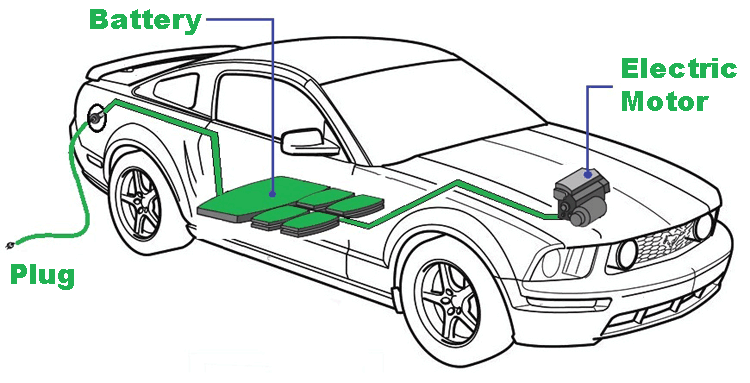
\includegraphics[width=0.7\textwidth]{EV.png}
	\caption{Esquem\'atico de un veh\'iculo electrico}
	\label{EV}
    \end{center}
\end{figure}

\noindent Siendo las baterías eléctricas la única fuente de energía en los 
\acrfull{VVEE}, éstas tienen un gran impacto en el desempeño de los mismos 
determinando la autonomía del vehículo. En base a este criterio, las 
baterías de iones de litio (\emph{Li-Ion}) resultan las más adecuadas para 
esta aplicación debido a su alta densidad energética, es decir, que este 
tipo de baterías tienen una gran capacidad para su reducido volumen a 
comparación de otras tecnologías. Para poder ser utilizados en
\acrshort{VVEE}, las baterías de Li-Ion son conectadas en forma de arreglos 
o packs de baterías en serie que permiten obtener mayores valores de tensión
y, otras, en paralelo para aumentar la capacidad del pack.

\subsection{Motivaci\'on del proyecto}

\noindent Una de las grandes problem\'aticas de las bater\'ias de Litio-ion 
reside en que se debe tener en cuenta ciertas precauciones a la hora de
implementarlas, debido a que las mismas son propensas a fallar al ser 
sobrecargadas, completamente descargadas u operadas fuera del
rango seguro de temperatura, tensi\'on o corriente, adem\'as, en un pack de 
bater\'ias conectadas en serie, se pueden manifestar pequeñas diferencias de 
capacidades a traves de todas las celdas, causado por tolerancias de
producci\'on o diferentes condiciones de operaci\'on, que tienden
a incrementar con cada ciclo de carga. Por \'ultimo, las bater\'ias
sufren un proceso de \emph{auto-descarga} (t\'ipicamente entre un
2-10\% dependiendo de la temperatura y el estado de carga de la misma). 
Si la distribuci\'on de temperatura a lo largo del pack es
heterog\'enea, las celdas con mayor temperatura tienden a una mayor
p\'erdida de capacidad provocando un desbalanceo de carga.
Esto trae varias consecuencias, entre ellas, se encuentran:

\begin{itemize}
    \item \textbf{Seguridad:} Si el voltaje máximo de carga es excedido por 
        unos cientos de milivoltios, puede provocar un embalamiento térmico, 
        derritiendo el pack de baterías y, por lo tanto, el dispositivo que 
        alimenta. En el peor de los casos puede explotar poniendo en riesgo el 
        bienestar del usuario.
    \item \textbf{Salud de la batería:} La degradación de la batería es 
        extremadamente sensible a la operación de la misma fuera de la zona 
        indicada. Si la temperatura de operación o la tensión máxima de carga 
        es excedida esto provoca una aceleración en la degradación de su vida 
        útil.
    \item \textbf{Autonomía:} Consideremos que el circuito de protección 
        detecta que una de las baterías se encuentra descargada a niveles 
        cercanos de operación insegura. En este caso, la protección frena la 
        descarga del pack por una sola celda y el resto se encuentran con 
        voltajes más altos y, por lo tanto, con un remanente de energía para 
        entregar a la carga desaprovechando la capacidad del pack entero.
\end{itemize}

Estas situaciones hacen necesario la implementación de un sistema de
administración de baterías (\emph{\acrshort{BMS}} por sus siglas en inglés
\acrlong{BMS}). En definitiva, un \acrshort{BMS} es un dispositivo encargado de
controlar las funciones vitales de las baterías para que operen de forma
correcta y segura, con el objetivo de otorgar seguridad al usuario y prolongar
la autonomía del vehículo. Las funciones más relevantes que llevan a cabo son:

\begin{itemize}
    \item Protección del pack para su operación en la región segura tanto 
        en tensión, corriente como también en temperatura.
    \item Ecualización de las celdas individuales del pack, es decir,
        controlar que la carga entre celdas sea uniforme
    \item Estimación del estado de carga del pack de batería 
        (\emph{\acrshort{SOC}} por sus siglas en ingl\'es \acrlong{SOC}).
    \item Estimación del estado de salud del pack de batería 
        (\emph{\acrshort{SOH}} por sus siglas en ingl\'es \acrlong{SOH}).
    \item Informar a la computadora central del vehículo los distintos 
        parámetros del pack de baterías.
\end{itemize}

\noindent Ademas de las problem\'aticas mencionadas anteriormente, en el mercado
actual se venden una gran variedad de \acrshort{BMS} con escasa documentaci\'on
sobre el mismo, dificultando su implementaci\'on con otros dispositivos, tales 
como computadoras centrales de veh\'iculos el\'ectricos hasta \acrshort{UPS}.

Por otro lado, existen solamente dos proyectos de c\'odigo/hardware abiertos
relacionados al desarrollo de \acrshort{BMS}, detallados a continuaci\'on.

\subsubsection{foxBMS}

\emph{foxBMS} \cite{foxbms} es un proyecto desarrollado por el Instituto de Sistemas
Integrados y Tecnolog\'ias de Dispositivos de la sociedad \emph{Fraunhofer} o
tambien llamado Fraunhofer IISB (del ingles \emph{\acrlong{IISB}}), una
organización de investigación alemana que comprende 72 institutos esparcidos por
todo el territorio alem\'an.

\noindent El desarrollo de este proyecto es el resultado de 15 años de
investigaci\'on en el \'area de energ\'ias renovables y es diseñado para 
administrar innovadores prototipos de sistemas de bater\'ias basados en la 
tecnolog\'ia iones de litio, desde pocas celdas conectadas en serie hasta 
centenares de kWh y kW, especialmente para sistemas que requieren altos niveles 
de fiabilidad.

\noindent El proyecto no tiene intenciones de ser usado de forma comercial en
productos ya que no cumple con estandards espec\'ificos y requieren determinados
certificados para ser vendidos en el mercado. Solamente cumple con el 
prop\'osito de ser una plataforma de ensayo y desarollo que provee todas las 
funcionalidades del manejo de la complejidad y tamaño de los sistemas de 
almacenamiento más avanzados al d\'ia de la fecha.

\noindent Si bien el mismo tiene extensa documentacion, originalmente fue
desarrollado para manejar packs de 12 a 18 celdas en serie, lo cual excede el
prop\'osito de la aplicaci\'on en cuestion por lo que no resulta viable para ser
implementado de forma directa. Tambien el hardware del proyecto es
extensivamente costoso y complejo, ya que implementa varios microcontroladores e
integrados dedicados hasta \acrshort{FPGA}s (del ingles, \emph{\acrlong{FPGA}}).

\subsubsection{openBMS}

A diferencia de \emph{foxBMS}, este proyecto fue desarrollado por ingenieros
independientes con el objetivo de diversificar los proyectos abiertos relativos
al tema en cuesti\'on.

\noindent El mismo busca desarrollar un \acrshort{BMS} capaz de manejar un
pack de bater\'ias de 4 a 96 celdas en serie, realizar el balanceo de las mismas 
y comunicar las variables del pack a traves del protocolo \acrshort{CAN}.

\noindent Si bien, se encuentran todos los archivos del proyecto a disposición
del publico, la documentaci\'on es muy escaza para ser implementado
f\'acilmente para un proyecto relacionado.

\noindent En definitiva, las motivaciones para llevar a cabo el presente trabajo
se basan en la complejidad en el manejo de grandes packs de
bater\'ias basadas en celdas de litio-ion y la falta de proyectos abiertos
disponibles relacionados al tema.

\subsection{Estructura del informe}

El informe se encuentra dividido en 6 secciones, en la Sección \ref{descripcion}
se realiza una descripci\'on en alto nivel del proyecto, detallando los
objetivos generales, las especificaciones y requerimientos del trabajo, a
continuaci\'on, se encuentra el fundamento te\'orico (Secci\'on \ref{teoria}),
donde se detalla el funcionamiento de una celda de litio-ion, los fundamentos
b\'asicos de modelados de celdas y algoritmos de estimaci\'on de carga, como
tambi\'en aquellos relacionados a la equalizaci\'on de celdas, adem\'as, se
presenta el desarrollo matem\'atico de mucho de los m\'etodos como tambi\'en una
comparativa, por ultimo se presentan las Secciones \ref{desarrollo} y
\ref{ensayos} donde se describe el desarrollo de la bater\'ia en si, en conjunto
con su modelo y algoritmos como tambi\'en su final implementaci\'on en un
sistema embebido con los ensayos realizados para validar el funcionamiento del
sistema. Finalmente, en la Secci\'on \ref{conclusiones} se describen las
conclusiones y futuros proyectos a continuar sobre el eje de estudio.

\section{Descripci\'on}\label{descripcion}

\subsection{Objetivos del proyecto}

Como solución a los problemas planteados, se propone desarrollar un
\acrshort{BMS} que cumpla con los siguientes requisitos:

\begin{itemize}
    \item Proteger el pack de baterías evitando que el mismo salga de su 
	zona de operación segura, tanto en tensión, corriente como en 
	temperatura, evaluando los umbrales correspondientes para las celdas de 
    Litio-Ion.
    \item Estimar el estado de carga en tiempo real.
    \item Balancear la carga entre celdas, priorizando el menor costo 
	energético posible del sistema y la mayor autonomía final del pack.
    \item Comunicar los parámetros fundamentales del pack a una computadora 
	central a través de algún protocolo estandarizado.
\end{itemize}

\noindent Para lograr estos objetivos, se plantea un estudio pormenorizado 
del estado del arte de la temática en cuestión procurando seleccionar las 
prácticas y metodologías más adecuadas para la solución del problema 
planteado, a partir de un estudio teórico. Finalmente se validará la 
solución elegida a partir de la implementación y ensayo de la solución 
desarrollada.

\subsection{Especificaciones}\label{proy_specs}

\noindent El sistema a implementar debe ser capaz de poder administrar un 
pack de bater\'ias de 6 m\'odulos conectados en serie, donde cada módulo est\'a 
compuesto por 3 celdas en paralelo encargado de: 

\begin{itemize}
    \item Sensar la tensión de las celdas individuales del pack y de la 
	corriente que circula desde y hacia el pack as\'i como tambi\'en 
	la temperatura media.
    \item Realizar el balanceo de los m\'odulos que componen a la bater\'ia.
    \item Proteger el mismo, desconectando el pack de bater\'ias de la carga
	frente a operaciones fuera de la zona segura.
    \item Estimar el estado de carga y detectar las celdas que se encuentran
	en desbalance utilizando una unidad de cómputo como por ejemplo, un
	microcontrolador o \acrshort{MCU} (del ingl\'es \emph{\acrlong{MCU}}).
    \item Controlar el proceso de carga del pack de bater\'ias.
    \item Comunicar las variables del sistema a una computadora central a
	trav\'es de un protocolo especificado
\end{itemize}

\noindent La descripción anterior se puede visualizar en el \acrfull{DB} de la
Figura \ref{bms}. Como puede observarse, el microcontrolador es el encargado de
comunicarse y comandar los módulos de protecci\'on, ecualizaci\'on y carga de 
la batería, como tambi\'en obtener variables de los mismos para poder estimar 
el \acrshort{SOC}, determinar el desbalanceo de una o m\'as celdas y tomar 
acci\'on al respecto, y por último, pero m\'as relevante, comandar las 
protecciones en caso de una falla y/o alerta de la batería. 
De forma simult\'anea, el mismo debe estar a cargo de comunicar las distintas 
variables del sistema a una computadora central.

\begin{figure}[h!]
    \begin{center}
	\begin{circuitikz}[european]
	    \draw (-4, -1) rectangle (-2, 1)[fill=blue!10!white];
	    \node at (-3, 0.2) {CPU};
	    \node at (-3, -0.2) {Central};
	    \draw [vecArrow] (-1.8, 0) to (-1, 0);
	    \draw [vecArrow] (-1.2, 0) to (-2, 0);

	    \draw (-1, -1) rectangle (1, 1)[fill=blue!10!white];
	    \node at (0, 0) {MCU};

	    \draw [blue,thin,dashed] (2.1, 2.5) rectangle (5.1, -2.5)[fill=blue!10!white];

	    \draw (2.2, 2.4) rectangle (5.0, 0.92)[fill=yellow!15!white];
	    \draw (2.2, 0.82) rectangle (5.0, -0.71)[fill=yellow!15!white];
	    \draw (2.2, -0.81) rectangle (5.0, -2.4)[fill=yellow!15!white];

	    \node at (3.6, 1.6) {Protección};           
	    \node at (3.6, -1.6) {Cargador};
	    \node at (3.6, 0) {Equalizaci\'on};
	    \draw [vecArrow] (1.2, 0) to (2.1, 0);
	    \draw [vecArrow] (1.5, 0) to (1, 0);

	    \draw (7, 2) -- (7, 2.2);
	    \draw (7, 2) to[battery1] (7, 1.6);
	    \draw (7, 1.4) -- (7, 1.6);
	    \draw (7, 1.4) to[battery1] (7, .9);            
	    \draw (7, .7) -- (7, .9);           
	    \draw (7, 0.7) to[battery1] (7, 0.2);           
	    \draw (7, 0.2) -- (7, -0.2);
	    \draw (7, -0.2) to[battery1] (7, -0.7);
	    \draw (7, -.7) -- (7, -.9);
	    \draw (7, -.9) to[battery1] (7, -1.4);
	    \draw (7, -1.4) -- (7, -1.6);
	    \draw (7, -1.6) to[battery1] (7, -2);
	    \draw (7, -2) -- (7, -2.2);

	    \draw (9, 2) -- (9, 2.2);
	    \draw (9, 2) to[battery1] (9, 1.6);
	    \draw (9, 1.4) -- (9, 1.6);
	    \draw (9, 1.4) to[battery1] (9, .9);            
	    \draw (9, .7) -- (9, .9);           
	    \draw (9, 0.7) to[battery1] (9, 0.2);           
	    \draw (9, 0.2) -- (9, -0.2);
	    \draw (9, -0.2) to[battery1] (9, -0.7);
	    \draw (9, -.7) -- (9, -.9);
	    \draw (9, -.9) to[battery1] (9, -1.4);
	    \draw (9, -1.4) -- (9, -1.6);
	    \draw (9, -1.6) to[battery1] (9, -2);
	    \draw (9, -2) -- (9, -2.2);

	    \draw (11, 2) -- (11, 2.2);
	    \draw (11, 2) to[battery1] (11, 1.6);
	    \draw (11, 1.4) -- (11, 1.6);
	    \draw (11, 1.4) to[battery1] (11, .9);          
	    \draw (11, .7) -- (11, .9);         
	    \draw (11, 0.7) to[battery1] (11, 0.2);     
	    \draw (11, 0.2) -- (11, -0.2);
	    \draw (11, -0.2) to[battery1] (11, -0.7);
	    \draw (11, -.7) -- (11, -.9);
	    \draw (11, -.9) to[battery1] (11, -1.4);
	    \draw (11, -1.4) -- (11, -1.6);
	    \draw (11, -1.6) to[battery1] (11, -2);
	    \draw (11, -2) -- (11, -2.2);

	    \draw (5.1, 0) to[short, -*] (7, 0);
	    \draw (7, 0) to[short, -*] (9, 0);
	    \draw (9, 0) to[short, -*] (11, 0);

	    \draw (7, 0.8) to[short, -*] (9, 0.8);
	    \draw (9, 0.8) to[short, -*] (11, 0.8);

	    \draw (7, 1.5) to[short, -*] (9, 1.5);
	    \draw (9, 1.5) to[short, -*] (11, 1.5);

	    \draw (7, 2.2) to[short, -*] (9, 2.2);
	    \draw (9, 2.2) to[short, -*] (11, 2.2);         

	    \draw (7, -0.8) to[short, -*] (9, -0.8);
	    \draw (9, -0.8) to[short, -*] (11, -0.8);

	    \draw (7, -1.5) to[short, -*] (9, -1.5);
	    \draw (9, -1.5) to[short, -*] (11, -1.5);

	    \draw (7, -2.2) to[short, -*] (9, -2.2);
	    \draw (9, -2.2) to[short, -*] (11, -2.2);           

	    \draw (5.1, 0.2) -- (6.2, 0.2) |- (7, 0.8) node at (7, .8){$\bullet$};
	    \draw (5.1, 0.4) -- (6, 0.4) |- (7, 1.5) node at (7, 1.5){$\bullet$};
	    \draw (5.1, 0.6) -- (5.8, 0.6) |- (7, 2.2) node at (7, 2.2){$\bullet$};

	    \draw (5.1, -0.2) -- (6.2, -0.2) |- (7, -0.8) node at (7, -.8){$\bullet$};
	    \draw (5.1, -0.4) -- (6, -0.4) |- (7, -1.5) node at (7, -1.5){$\bullet$};
	    \draw (5.1, -0.6) -- (5.8, -0.6) |- (7, -2.2) node at (7, -2.2){$\bullet$};

	    \draw [dashed] (-1.2, 2.6) rectangle (5.2, -2.6);
	    \draw node at (-.8, 2.8){BMS};

	    \draw [dashed] (6.5, 2.4) rectangle (11.5, -2.4);

	    \draw node at (8.2, 2.6) {Pack de Baterías 6s3p};

	    \draw (13, 1) to[R=$Z$] (13, -1);

	    \draw (11, 2.2) -- (12, 2.2)
	    |- (12, 1.5) -- (13, 1.5) |- (13,1) node at (12, 1.5){$\bullet$};

	    \draw (11, -2.2) -- (12, -2.2)
	    |- (12, -1.5) -- (13,-1.5) |- (13,-1) node at (12, -1.5){$\bullet$};

	    \draw node at (12.8, 1){+};
	    \draw node at (12.8, -1){-};  
	\end{circuitikz}
    \end{center}
    \caption{Diagrama en Bloques del \acrshort{BMS} y el pack de baterías}
    \label{bms}
\end{figure}

\section{Aspectos Te\'oricos}\label{teoria}

input(state\_of\_art)

\section{Desarrollo}\label{desarrollo}

En \'esta secci\'on se explaya el desarrollo matem\'atico y la implementaci\'on 
f\'isica del \acrshort{BMS}, incluyendo el pack de bater\'ias, el modelo 
matem\'atico de la celda de litio-ion junto a sus algortimos de estimaci\'on de 
\acrshort{SOC} y ecualizaci\'on de celdas, mostrando los resultados de las
simulaciones y, finalmente, el desarrollo del hardware y firmware necesario para
implementar los distintos componentes del sistema en un sistema f\'isico real.

\subsection{Espíritu del proyecto}

El desarrollo del proyecto se funda sobre bases de espíritu colarborativas, bajo
la filosofía de codigo abierto y de software libre. Fuera del paragua de alguna
licencia en particular. Tanto los archivos fuentes del proyecto, de software y
hardware, como la extensa y profunda documentación del mismo se encuentran
disponibles para quienes deseen estudiarlos, modificarlos, ejecutarlos y
redistribuirlos citando la fuente debidamente. 

El proyecto no persigue fines comerciales ni onerosos de ningún tipo y pretende
ser una nueva pieza en el reducido ecosistema de los \acrshort{BMS}s de
codigo/hardware abierto.

El hardware y el software desarrollado se orientan a servir como plataforma de
ensayo y desarrollo de futuros proyectos que partan de este \acrshort{BMS}. Con
el objetivo de que la disposición de la documentación funcione como la
herramienta que lo permita.

\subsection{Pack de bater\'ias}\label{battery_pack}

Como se menciona en la secci\'on \ref{proy_specs}, el pack de bater\'ias a
controlar posee 6 m\'odulos conectados en serie, donde cada m\'odulo est\'a
compuesto por 3 celdas de litio-ion conectadas en paralelo. En este caso, el pack
de bater\'ias est\'a conformado por celdas de litio-ion modelo NCR18650PF. La
arquitectura del pack se puede observar en la Figura \ref{pack_bateria} y una
im\'agen de la celda se muestra en la Figura \ref{foto_bateria}

\begin{figure}[h!]
    \begin{subfigure}[b]{.5\textwidth}
	\begin{center}
	    \begin{minipage}[c]{0.45\textwidth}
		\centering
		\begin{circuitikz}[european]

		    \draw (7, 2) -- (7, 2.2);
		    \draw (7, 2) to[battery1] (7, 1.6);
		    \draw (7, 1.4) -- (7, 1.6);
		    \draw (7, 1.4) to[battery1] (7, .9);			
		    \draw (7, .7) -- (7, .9);			
		    \draw (7, 0.7) to[battery1] (7, 0.2);			
		    \draw (7, 0.2) -- (7, -0.2);
		    \draw (7, -0.2) to[battery1] (7, -0.7);
		    \draw (7, -.7) -- (7, -.9);
		    \draw (7, -.9) to[battery1] (7, -1.4);
		    \draw (7, -1.4) -- (7, -1.6);
		    \draw (7, -1.6) to[battery1] (7, -2);
		    \draw (7, -2) -- (7, -2.2);

		    \draw (9, 2) -- (9, 2.2);
		    \draw (9, 2) to[battery1] (9, 1.6);
		    \draw (9, 1.4) -- (9, 1.6);
		    \draw (9, 1.4) to[battery1] (9, .9);			
		    \draw (9, .7) -- (9, .9);			
		    \draw (9, 0.7) to[battery1] (9, 0.2);			
		    \draw (9, 0.2) -- (9, -0.2);
		    \draw (9, -0.2) to[battery1] (9, -0.7);
		    \draw (9, -.7) -- (9, -.9);
		    \draw (9, -.9) to[battery1] (9, -1.4);
		    \draw (9, -1.4) -- (9, -1.6);
		    \draw (9, -1.6) to[battery1] (9, -2);
		    \draw (9, -2) -- (9, -2.2);

		    \draw (11, 2) to[battery1] (11, 1.6);
		    \draw (11, 1.4) -- (11, 1.6);
		    \draw (11, 1.4) to[battery1] (11, .9);			
		    \draw (11, .7) -- (11, .9);			
		    \draw (11, 0.7) to[battery1] (11, 0.2);		
		    \draw (11, 0.2) -- (11, -0.2);
		    \draw (11, -0.2) to[battery1] (11, -0.7);
		    \draw (11, -.7) -- (11, -.9);
		    \draw (11, -.9) to[battery1] (11, -1.4);
		    \draw (11, -1.4) -- (11, -1.6);
		    \draw (11, -1.6) to[battery1] (11, -2);
		    \draw (11, -2) -- (11, -2.2);

		    \draw (7, 0) -- (9, 0);
		    \draw (9, 0) -- (11, 0);

		    \draw (7, 0.8) -- (9, 0.8);
		    \draw (9, 0.8) -- (11, 0.8);

		    \draw (7, 1.5) -- (9, 1.5);
		    \draw (9, 1.5) -- (11, 1.5);

		    \draw (7, 2.2) -- (9, 2.2);
		    \draw (9, 2.2) -- (11, 2.2);			

		    \draw (7, -0.8) -- (9, -0.8);
		    \draw (9, -0.8) -- (11, -0.8);

		    \draw (7, -1.5) -- (9, -1.5);
		    \draw (9, -1.5) -- (11, -1.5);

		    \draw (7, -2.2) -- (9, -2.2);
		    \draw (9, -2.2) -- (11, -2.2);			

		    \draw [dashed] (6.5, 2.4) rectangle (11.5, -2.4);

		    \draw node at (8.2, 2.6) {Pack de Baterías 6s3p};
		\end{circuitikz}
	    \end{minipage}
	\end{center}
	\caption{Esquemático de la arquitectura del pack de baterías.}
	\label{pack_bateria}
    \end{subfigure}%
    \begin{subfigure}[b]{.45\textwidth}
	\centering
	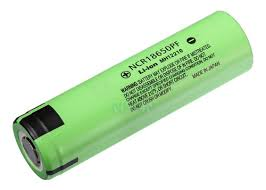
\includegraphics[width=0.7\textwidth]{18650.jpg}
	\caption{Foto celda NCR18650PF.}
	\label{foto_bateria}
    \end{subfigure}
    \caption{Pack 6s3p y Celda NCR18650PF.}
    \label{pack}
\end{figure}
\FloatBarrier

\newpage

\subsubsection{Celda NCR18650PF}

La celda de litio-ion 18650 fue originalmente diseñada para ser utilizada en
bater\'ias de notebooks pero debido a su amplia versatilidad su uso se
expandi\'o hasta ser implementados en \acrshort{VVEE}s. \'Estas bater\'ias se
caracterizan por su tamaño reducido de 18mm de di\'ametro por 65mm de alto,
caracteristicas que le dan su nombre. En el mercado actual, se pueden encontrar
diferentes versiones del mismo modelo debido a que cada uno posee una
composici\'on qu\'imica diferente, dando lugar a las distintas caracter\'isticas
de capacidad y voltaje que se descrien a continuaci\'on:

\begin{itemize}
    \item \textbf{LiFePO4}: Fosfato de hierro y litio o tambi\'en conocidas como
        IFR, LFP o Li-fosfato.
    \item \textbf{LiMn2O4}: Oxido de litio manganesio o tambi\'en conocidas como
        IMR, LMO o Li-manganesio.
    \item \textbf{LiNiMnCoO2}: Litio manganesio n\'iquel o tambi\'en conocidas como
        INR o NMC
    \item \textbf{LiNiCoAl2}: Oxido de Litio n\'iquel cobalto aluminio o
        tambi\'en conocidas como NCA o Li-aluminio.
    \item \textbf{LiNiCoO2}: \'Oxido de litio n\'iquel cobalto o tambi\'en
        conocidas como NCO.
    \item \textbf{LiCoO2}: \'Oxido de litio cobalto o tambi\'en conocido como
        ICR, LCO o Li-cobalto.
\end{itemize}

En este caso, la celda NCR18650PF se caracteriza por su cátodo, cuya composición 
química se basa en el óxido de litio níquel cobalto aluminio 
($\mathrm{LiNiCoAlO_2}$) y, según su hoja de datos \cite{18650pf}, sus 
carateristicas electricas se pueden observar en la Tabla \ref{ncr18650pf_table}.

\begin{table}[h]
    \begin{center}
	\begin{tabular}{|c|l|}
	    \hline
	    \multicolumn{2}{|c|}{Especificaciones el\'ectricas}                          \\ \hline
	    \textbf{Capacidad Específica}                 & 2700mAh                            \\ \hline
	    \multirow{2}{*}{\textbf{Capacidad}}           & Mínimo: 2750mAh                    \\ \cline{2-2} 
	    & Tipico: 2900mAh                    \\ \hline
	    \textbf{Corriente de Descarga Máxima}         & 10000mAh($\sim$3.5C)               \\ \hline
	    \textbf{Rango operativo de tensión}           & 2.5V - 4.2V                        \\ \hline
	    \textbf{Voltaje Nominal}                      & 3.6V                               \\ \hline
	    \textbf{Charga}                               & CC-CV, Std. 1375mA, 4.20V, 4.0 hrs \\ \hline
	    \textbf{Peso}                                 & 48g                              \\ \hline
	    \multirow{3}{*}{\textbf{Temperatura}}         & Carga: 0 a 45C                     \\ \cline{2-2} 
	    & Descarga: -20 a 60C                \\ \cline{2-2} 
	    & Almacenaje: -20 a 50C              \\ \hline
	    \multirow{2}{*}{\textbf{Densidad Energética}} & Volum\'etrica: 577Wh/l               \\ \cline{2-2} 
	    & Gravim\'etrica: 207wh/kg             \\ \hline
	\end{tabular}%
	\caption{Especificaciones el\'ectricas de una celda de litio NCR18650PF}
	\label{ncr18650pf_table}
    \end{center}
\end{table}

Por el otro lado, \cite{18650pf} también nos provee curvas significativas, de su
operaci\'on como por ejemplo, la curva de carga \emph{(Fig. \ref{cc_cv_18650})}, 
la curva de descarga para distintas corrientes 
\emph{(Fig. \ref{descarga_18650})} y la curva del ciclo de vida típico de la 
batería \emph{(Fig. \ref{life_cycle_18650})}.

La elecci\'on de \'este tipo de celda se debe a principalmente a que el pack a
controlar ya utiliza \'este modelo y, por el otro lado, ya existe un set de 
datos abiertos \cite{Kollmeyer2018} de distintos ensayos sobre el
mismo, con el cual se pueden desarrollar e investigar distintos modelos y 
simulaciones. En la Figura \ref{pack_bat_foto} se puede observar 

\begin{figure}[h!]
    \begin{subfigure}[t]{.5\textwidth}
	%   		\centering
	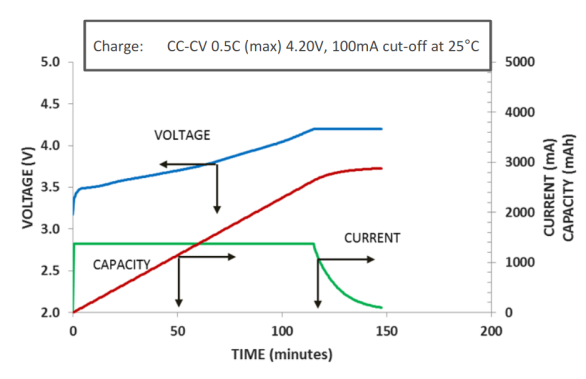
\includegraphics[width=0.9\textwidth]{cc_cv_18650.png}
	\caption{Curva de carga.}
	\label{cc_cv_18650}
    \end{subfigure}%
    ~ 
    \begin{subfigure}[t]{.5\textwidth}
	%    		\centering
	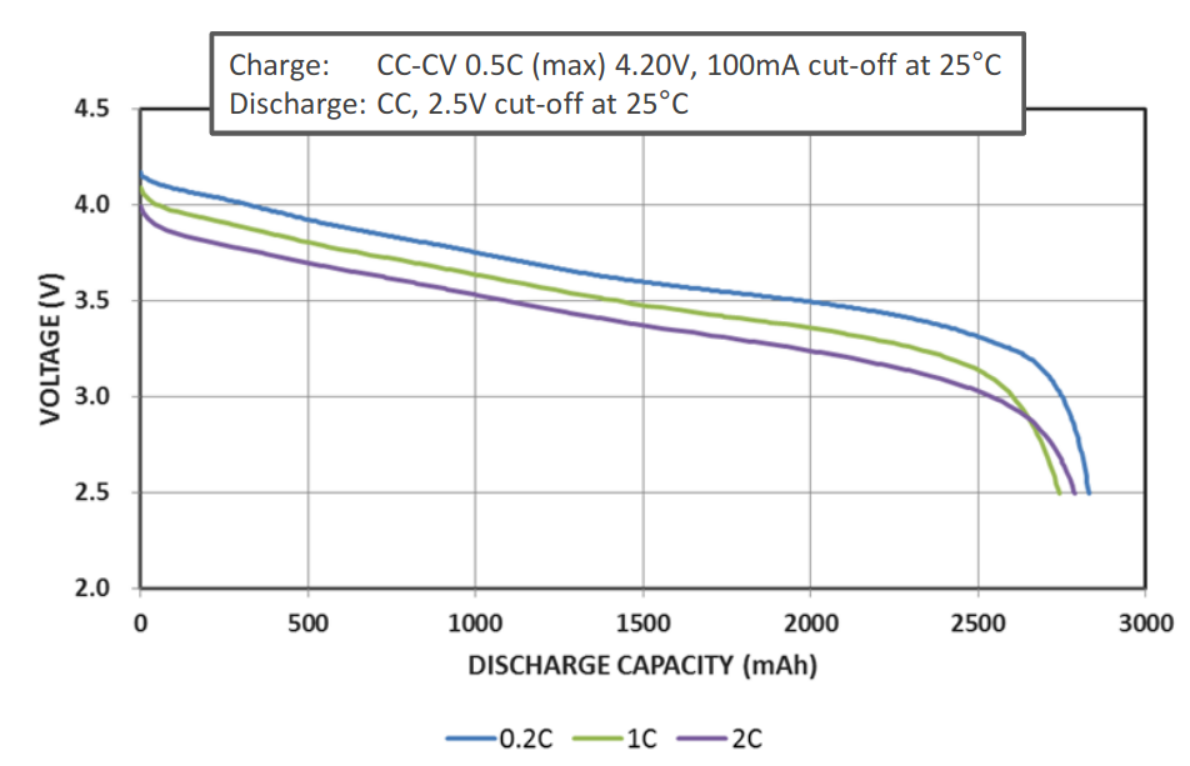
\includegraphics[width=0.9\textwidth]{discharge_18650.png}
	\caption{Curva de descarga en base a distintas corrientes de descarga (0.5C,
	1C, 1.5C y 2C)}
	\label{descarga_18650}
    \end{subfigure}
    ~ 
    \begin{centering}
	\begin{subfigure}[t]{1\textwidth}
	    \centering
	    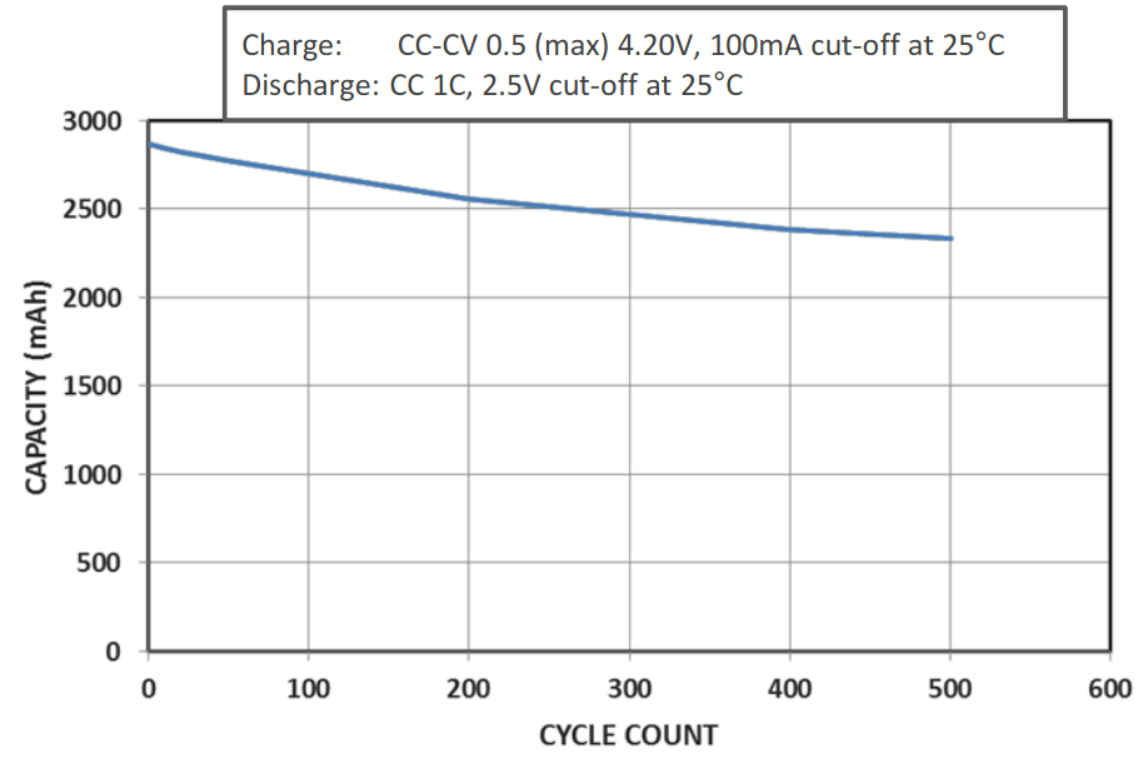
\includegraphics[width=0.4\textwidth]{life_cycle_18650.png}
	    \caption{Curva del ciclo de vida de una celda 18650}
        \label{life_cycle_18650}
	\end{subfigure}
    \end{centering}
    \caption{Curvas sgnificativas celda Panasonic 18650PF}
    \label{curvas_sign_18650}
\end{figure}

\newpage

\subsubsection{Ensamblado del pack}

El pack de bater\'ias es ensamblado utilizando soportes encastrables \emph{(Fig.
\ref{soporte_18650})} impresos utilizando una impresora 3D, donde cada celda es
conectada entre s\'i utilizando una banda de níquel y la conexi\'on es realizada 
por una soldadora de puntos manual. Esto es debido a dos motivos importantes, en 
primer instancia el tiempo en la aplicaci\'on de temperatura, por parte de la 
soldadura de puntos, es muy corto evitando problemas t\'ermicos de la celda 
durante el proceso de ensamblado. Por el otro lado, la banda de níquel tiene 
propiedades que benefician al ensamblado del pack, por ejemplo:

\begin{itemize}
    \item Protecci\'on en contra a la corrosi\'on.
    \item Buena conductividad el\'ectrica. El Niquel tiene la mitad de la
        resistencia el\'ectrica que el acero 1010.
    \item Buena resistencia mec\'anica.
    \item Bajo costo.
    \item Es soldable, por lo que se puede aplicar una soldadura de punto entre
        la tira de n'iquel y los electrodos de la celda.
\end{itemize}

\begin{figure}[h!]
    \begin{center}
        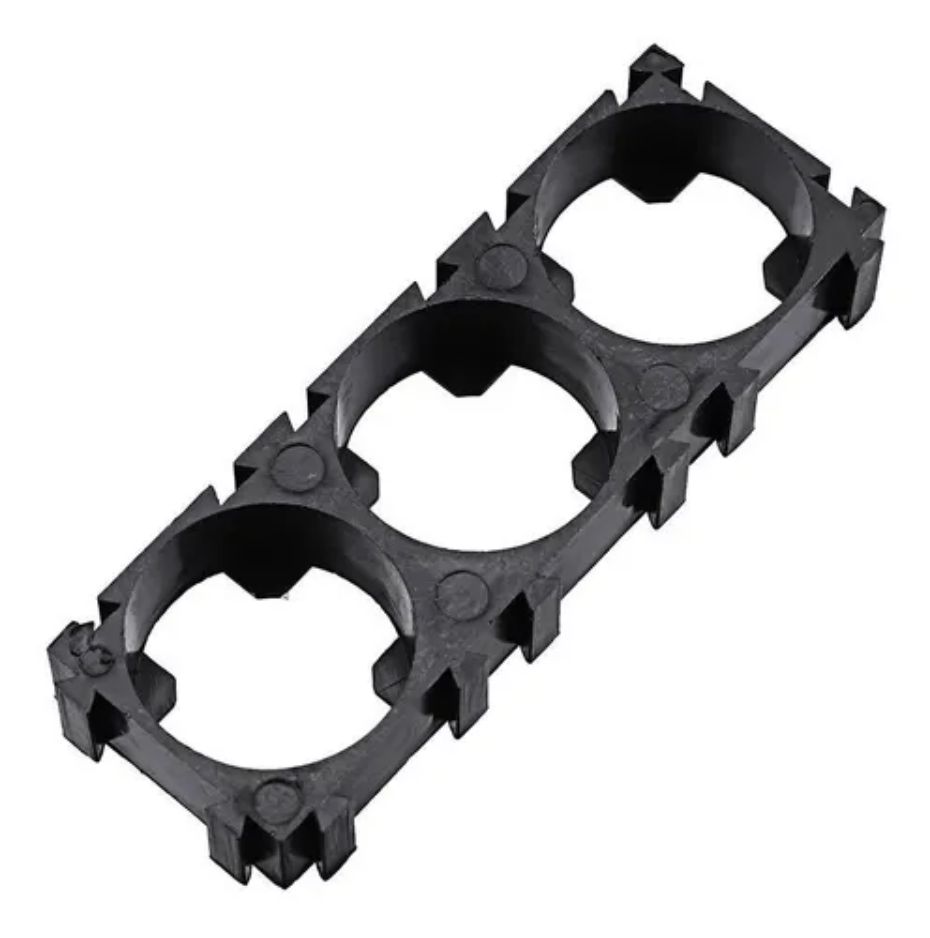
\includegraphics[width=0.45\textwidth]{soporte_18650.png}
        \caption{Soporte encastrable para celdas 18650}
        \label{soporte_18650}
    \end{center}
\end{figure}

Por el otro lado, a cada m\'odulo conectado en serie se le suelda un cable en
bornes de cada electrodo que va conectado a un conector JST-XH-2.50 para poder
acceder f\'acilmente al voltaje de cada m\'odulo del pack de bater\'ias. El pack
ensamblado se puede observar en las Figuras \ref{battery_top}-\ref{battery_side}

\begin{figure}[h!]
    \begin{subfigure}[b]{.3\textwidth}
	\begin{center}
        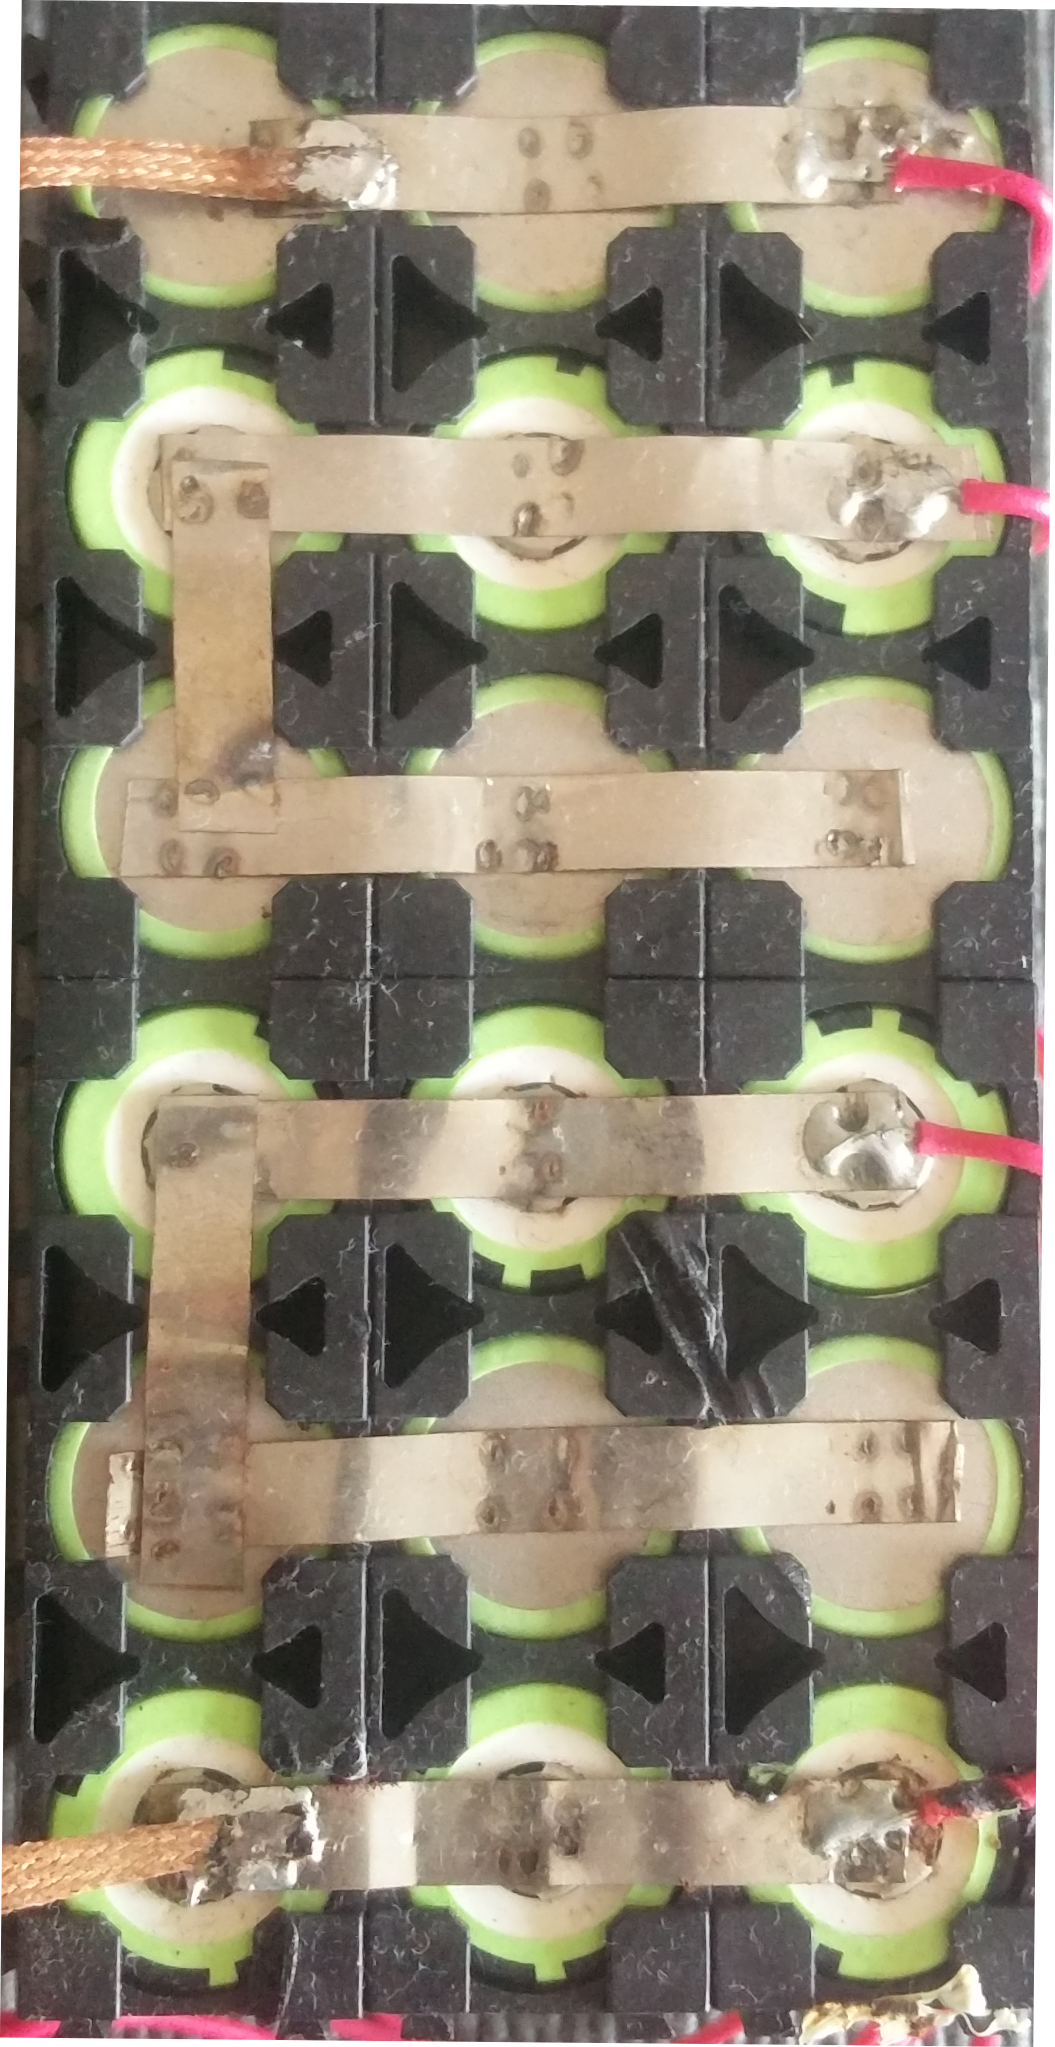
\includegraphics[width=.9\textwidth]{battery_top.png}
	\end{center}
    \caption{Imagen superior del pack de bater\'ias 6s3p. 
    }
	\label{battery_top}
    \end{subfigure}%
    \begin{subfigure}[b]{.3\textwidth}
	\centering
	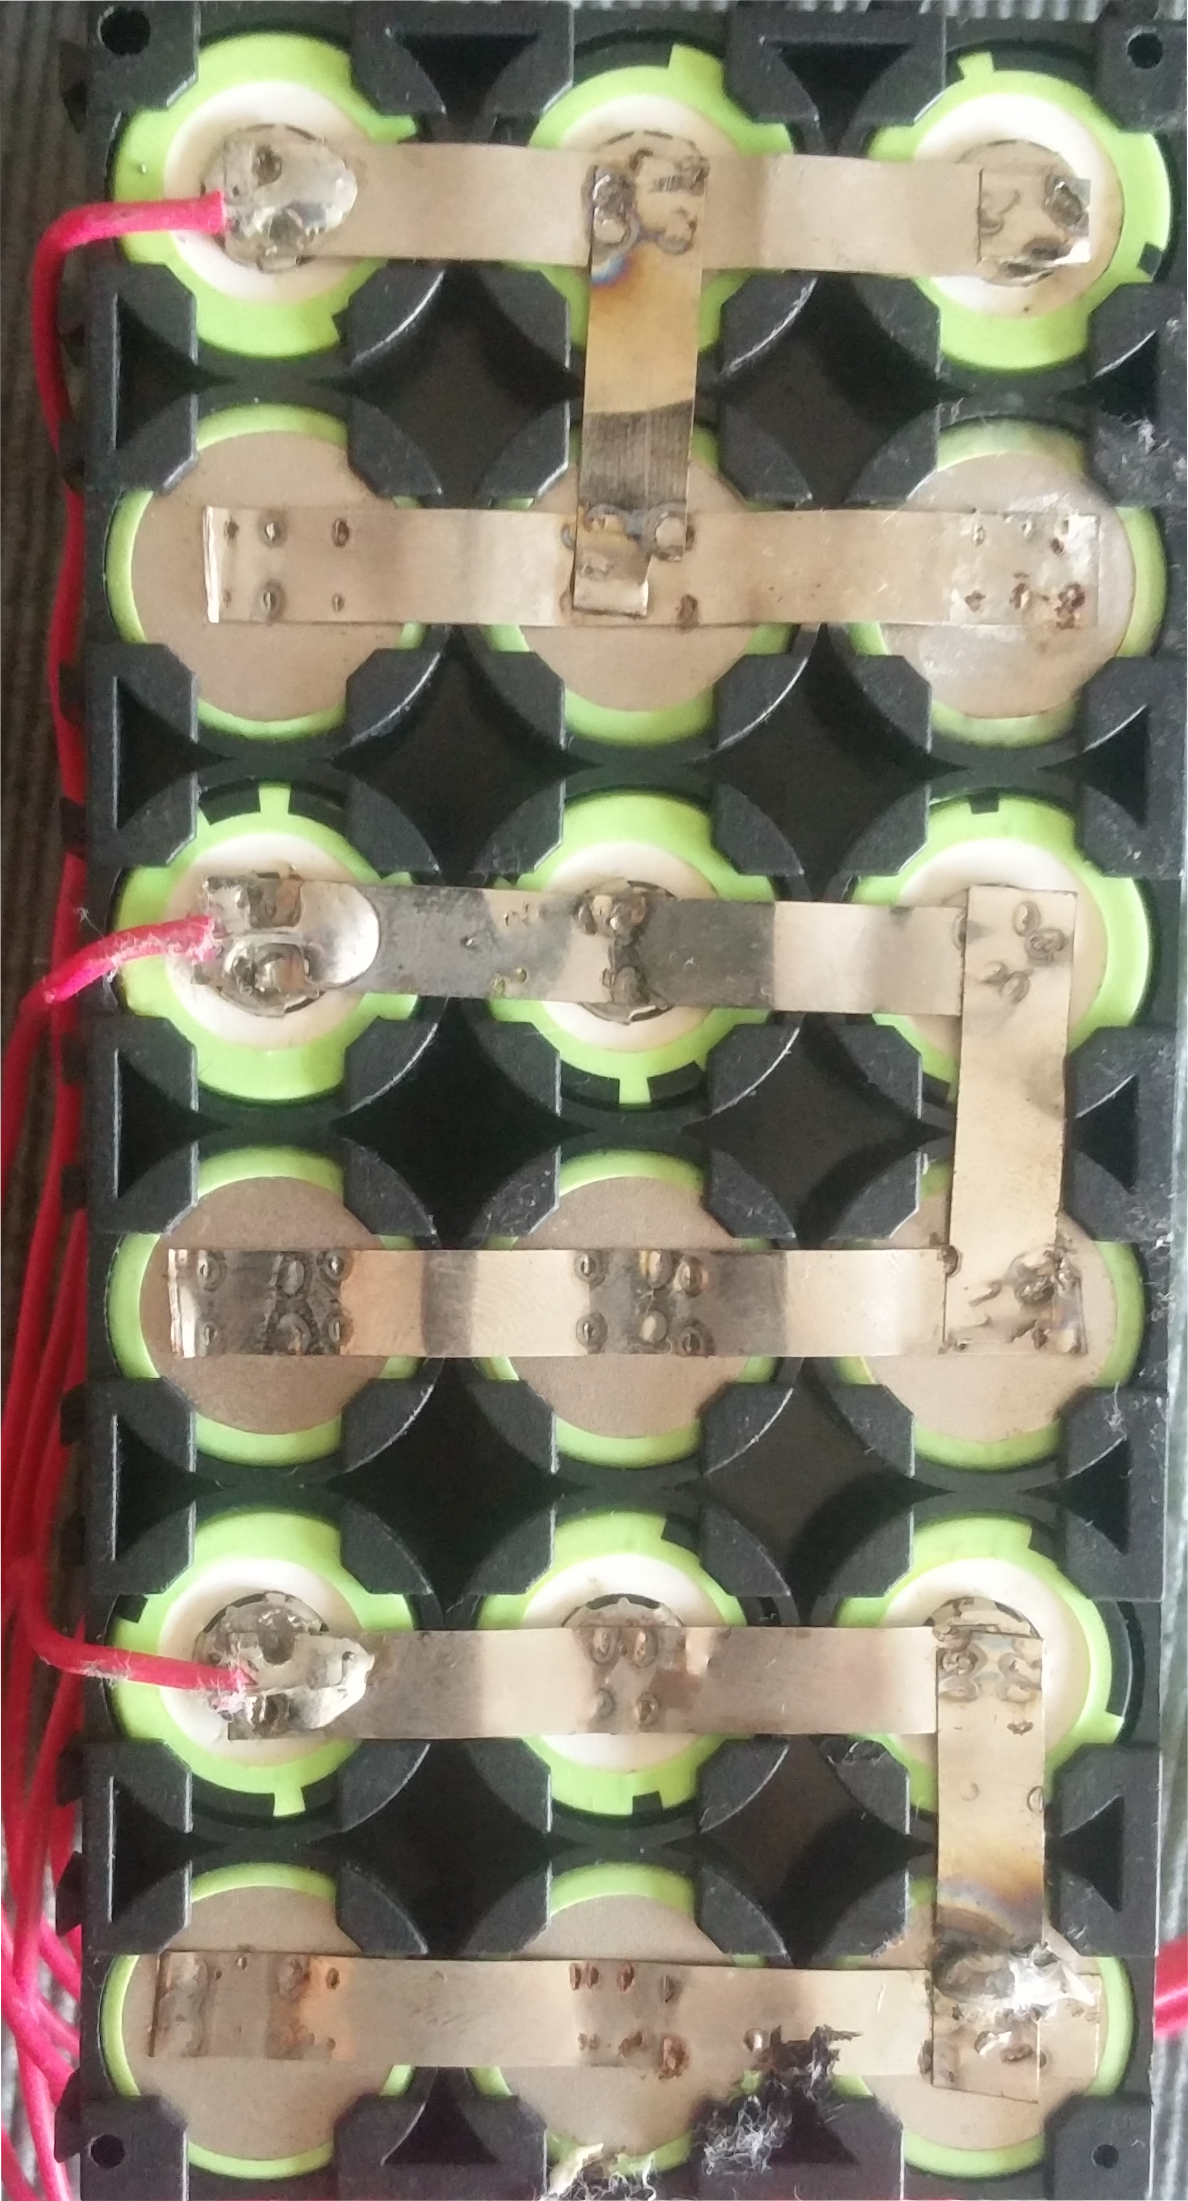
\includegraphics[width=.9\textwidth]{battery_bot.png}
	\caption{Imagen inferior del pack de bater\'ias 6s3p.}
	\label{battery_bot}
    \end{subfigure}
    \begin{subfigure}[b]{.3\textwidth}
	\centering
	\includegraphics[width=.9\textwidth]{batt_side.png}
	\caption{Imagen lateral del pack de bater\'ias 6s3p. En esta foto se puede
    apreciar el conector JST}
	\label{battery_side}
    \end{subfigure}
\end{figure}

\newpage

\subsubsection{Caracter\'isticas del pack}\label{caract_pack}

Como resultado obtenemos un pack de bater\'ias con las siguientes
caracter\'isticas:

\begin{itemize}
    \item Voltaje nominal de salida: 21.6V
    \item Voltaje m\'aximo de salida: 25.2V
    \item Voltaje m\'inimo de salida: 15V
    \item Capacidad t\'ipica: 8700mAh
    \item Capacidad m\'inima: 8250mAh
    \item Corriente de carga m\'axima: 4.35A
    \item Corriente de descarga m\'axima: 17.4A (2C)
\end{itemize}

\subsection{Modelo de la celda de litio-ion}\label{dev_batt_model}

Contar con un modelo matemático preciso que describa fehacientemente el
comportamiento y la dinámica de una celda de Ion-Litio es condición sine qua non
para la implementación exitosa de los algoritmos de estimación del
\acrshort{SOC} y de ecualización basados en el filtro de Kalman.

El modelado de una celda de litio puede ser abordado desde distintas
perspectivas y con difetentes herramientas matemáticas de acuerdo a los fines
que se persigan. La necesidad de conjugar un modelo de exactitud elevada que no
represente una carga computacional imposible de procesar en tiempo real en un
microcontrolador nos ha llevado a adoptar un modelo de segundo orden basado en
un circuito eléctrico siguiendo \cite{spagnol_kalman}, también conocido como
modelo de Randles de segundo orden, que se encuentra representado por el
esquem\'atico de la Figura \ref{randles_2rc} cuya parametrizaci\'on se describe
en la Secci\'on \ref{param_18650pf}.

\begin{figure}[h!]
    \begin{center}
	    \ctikzset{bipoles/length=1.0cm}
	    \ctikzset{bipoles/resistor/height=.3}

	    \begin{circuitikz}[american]
		\draw (0,0) to[R=$R_0$] (2,0) -- (2,-1) to[R=$R_1$] (4,-1) -- (4,0);
        \draw (2,0) -- (2, 1) to[C=$C_1$,v=$V_{C1}$] (4, 1) -- (4,0);
        \draw (4,0) to[short] (5, 0) -- (5, 1) to[C=$C_2$,v=$V_{C2}$] (7, 1) -- (7, 0);
		\draw (5,0) -- (5,-1) to[R=$R_2$] (7,-1) -- (7,0) to[short,f=$i$] (8,0);
        \draw (0,0) to[battery2=$V_{OCV}(SOC)$] (0,-3) -- (8,-3); 
        \draw  (8,0) to [open,v=$V_{out}$,invert] (8,-3);
	    \end{circuitikz}
        \caption{Circuito de Randles de Segundo Orden.}
        \label{randles_2rc}
    \end{center}
\end{figure}
\FloatBarrier

De acuerdo a la figura \ref{randles_2rc}, la salida del modelo es descripta por
la Ecuación \ref{eq:Vout_randles_2rc}

\begin{equation}
    V_{out}(t)=V_{OCV}(SOC)-(V_{R0}(t)+V_{C1}(t)+V_{C2}(t))
    \label{eq:Vout_randles_2rc}
\end{equation}

El modelo puede ser reescrito en el dominio de la transformada de Laplace como: 

\begin{align}
    \begin{split}
    V_{out}(t)&=V_{OCV}(SOC)-(R_{0}+\frac{R_{1}}{(1+sR_{1}C_{1})}\frac{R_{2}}{(1+sR_{2}C_{2})})i(t)\\
    &=V_{OCV}(SOC)-(R_{0}+\frac{K_{p}(1+sT_{2})}{(1+sT_{P1})(1+sT_{P2})})i(t)\\
    &=V_{OCV}(SOC)-R_{0}i(t)-G(s)i(t)
    \end{split}
       \label{eq:L_Vout_randles_2rc}
\end{align}

\subsubsection{Parametrizaci\'on del modelo}\label{param_18650pf}

La estimaci\'on de par\'ametros es com\'unmente usado para ajustar la respuesta 
de un modelo a los datos experimentales de un modelo f\'isico. En el caso de 
las celdas de litio-ion, los datos experimentales provienen de curvas
\acrfull{HPPC}. Este proceso involucra reiteradas simulaciones del modelo
matem\'atico planteado junto con la implementación y uso de un algoritmo de
optimizaci\'on num\'erico. De esta forma, el proceso de optimizaci\'on busca
ajustar los par\'ametros del modelo para minimizar el error entre los datos
experimentales y los resultados de las simulaciones realizadas.

En este caso, la curva \acrshort{HPPC}, que contiene un conjunto de pulsos de
carga/descarga, provee una representaci\'on con un alto nivel de fidelidad sobre
el comportamiento din\'amico de la bater\'ia, en m\'ultiples niveles del
\acrshort{SOC}. Para reflejar este comportamiento en el modelo planteado en la
Figura \ref{randles_2rc}, se requieren elementos circuitales no lineas flexibles
a las condiciones de operaci\'on y estados de la celda. Para realizar esto,
com\'unmente se emplean tablas de b\'usqueda (\acrshort{LUT}, del ingl\'es
\emph{\acrlong{LUT}}).

En este caso, los datos experimentales a analizar provienen de 
\cite{Kollmeyer2018}, que son descriptos en la siguiente secci\'on.

\subsubsection{Descripci\'on del set de datos}

El set de datos de  es un conjunto de ensayos realizados en 
la Universidad de Wisconsin-Madison por el Dr. Phillip Kollmeyer. Estos ensayos 
son realizados sobre una celda Panasonic NCR18650PF de 2.9Ah en una c\'amara 
t\'ermica con una celda de carga marca \emph{Digatron} que cuenta con una 
capacidad de descarga de 25A a 18V.

Los ensayos fueron realizados bajo 5 temperaturas diferents, en donde la
bater\'ia es cargada a 4.2V@2.9A despu\'es de cada ciclo. Sobre la celda se
ejecutaron los siguientes ciclos:

\begin{enumerate}
    \item 20 ciclos de Ensayo de carga y descarga.
    \item Cinco ensayos \acrshort{HPPC} a 0.5C, 1C, 2C, 4C y 6C realizados a
        intervalos de 5\% de \acrshort{SOC} en todo el rango de la capacidad de
        la celda.
    \item Ensayos \acrshort{EIS} en un rango de frecuencia de 1MHz a 100Hz, con
        el mismo paso y rango de \acrshort{SOC} que el punto anterior.
    \item Nueve ciclos de conducci\'on (del ing\'es, \emph{drive cycles})
        distintos, diseñados para poder capturar din\'amicas adicionales que no
        se pueden manifestar en el ensayo \acrshort{HPPC}.
    \item Los pasos 3 a 5 son ensayados nuevamente bajo 5 temperaturas distintas
        (25\degree C, 10\degree C, 0\degree C, -10\degree C y -20\degree C)
    \item Los nueve ciclos de conducci\'on se repiten con una temperatura
        inicial de -20\degree C, donde despu\'es se la permite evolucionar en
        funci\'on del calor generado por las bater\'ias.
    \item Los primeros 3 ciclos se repiten con la c\'amara a una temperatura
        inicial de -20\degree C.
    \item Los nueve ciclos de conducci\'on se ejecutan nuevamente con una
        temperatura inicial de 10\degree C.
    \item Los ciclos 1 a 4 se repiten con una temperatura inicial de 10\degree
        C.
    \item Finalmente, se le realizaron 10 ciclos de descarga a 1C con una
        temperatura ambiente de 25\degree C, seguidos por dos ensayos de
        referencia de capacidad demostrando que la capacidad m\'axima decae de
        2.8Ah a 2.3Ah despu\'es de correr todos los ensayos enumerados
        anteriormente.
\end{enumerate}

\subsubsubsection{Ensayos HPPC}\label{ensayo_HPPC}

El ensayo \acrshort{HPPC} es una metodología utilizada para poder caratcerizar
la dinámica de una celda. El perfil de ensayo \acrshort{HPPC} del dataset
\cite{Kollmeyer2018} presenta múltiples pulsos de descarga y de relajación a
intervalos de 5\% del estado de carga (\acrshort{SOC}). El ensayo es llevado a
cabo bajo el estricto control de la temperatura del electrolito y de la
corriente de descarga. Los pulsos de descarga son apreciablemente cortos
respecto del periodo de relajación siendo su duración de 1s y 2 minutos
respectivamente, con la intención de que el pulso del ensayo perturve la celda
sin modificar su estado de carga.

Para poder poblar las tablas de busqueda del modelo es necesario contar con
información experimental suficiente que ejercite cada uno de los parámetros que
las componen. Son las curvas del ensayo \acrshort{HPPC}, que pueden observarse
en la Figura \ref{hppc_kollmeyer}, las que nos brindan la imformación necesaria.

\begin{figure}[h!]
    \begin{center}
        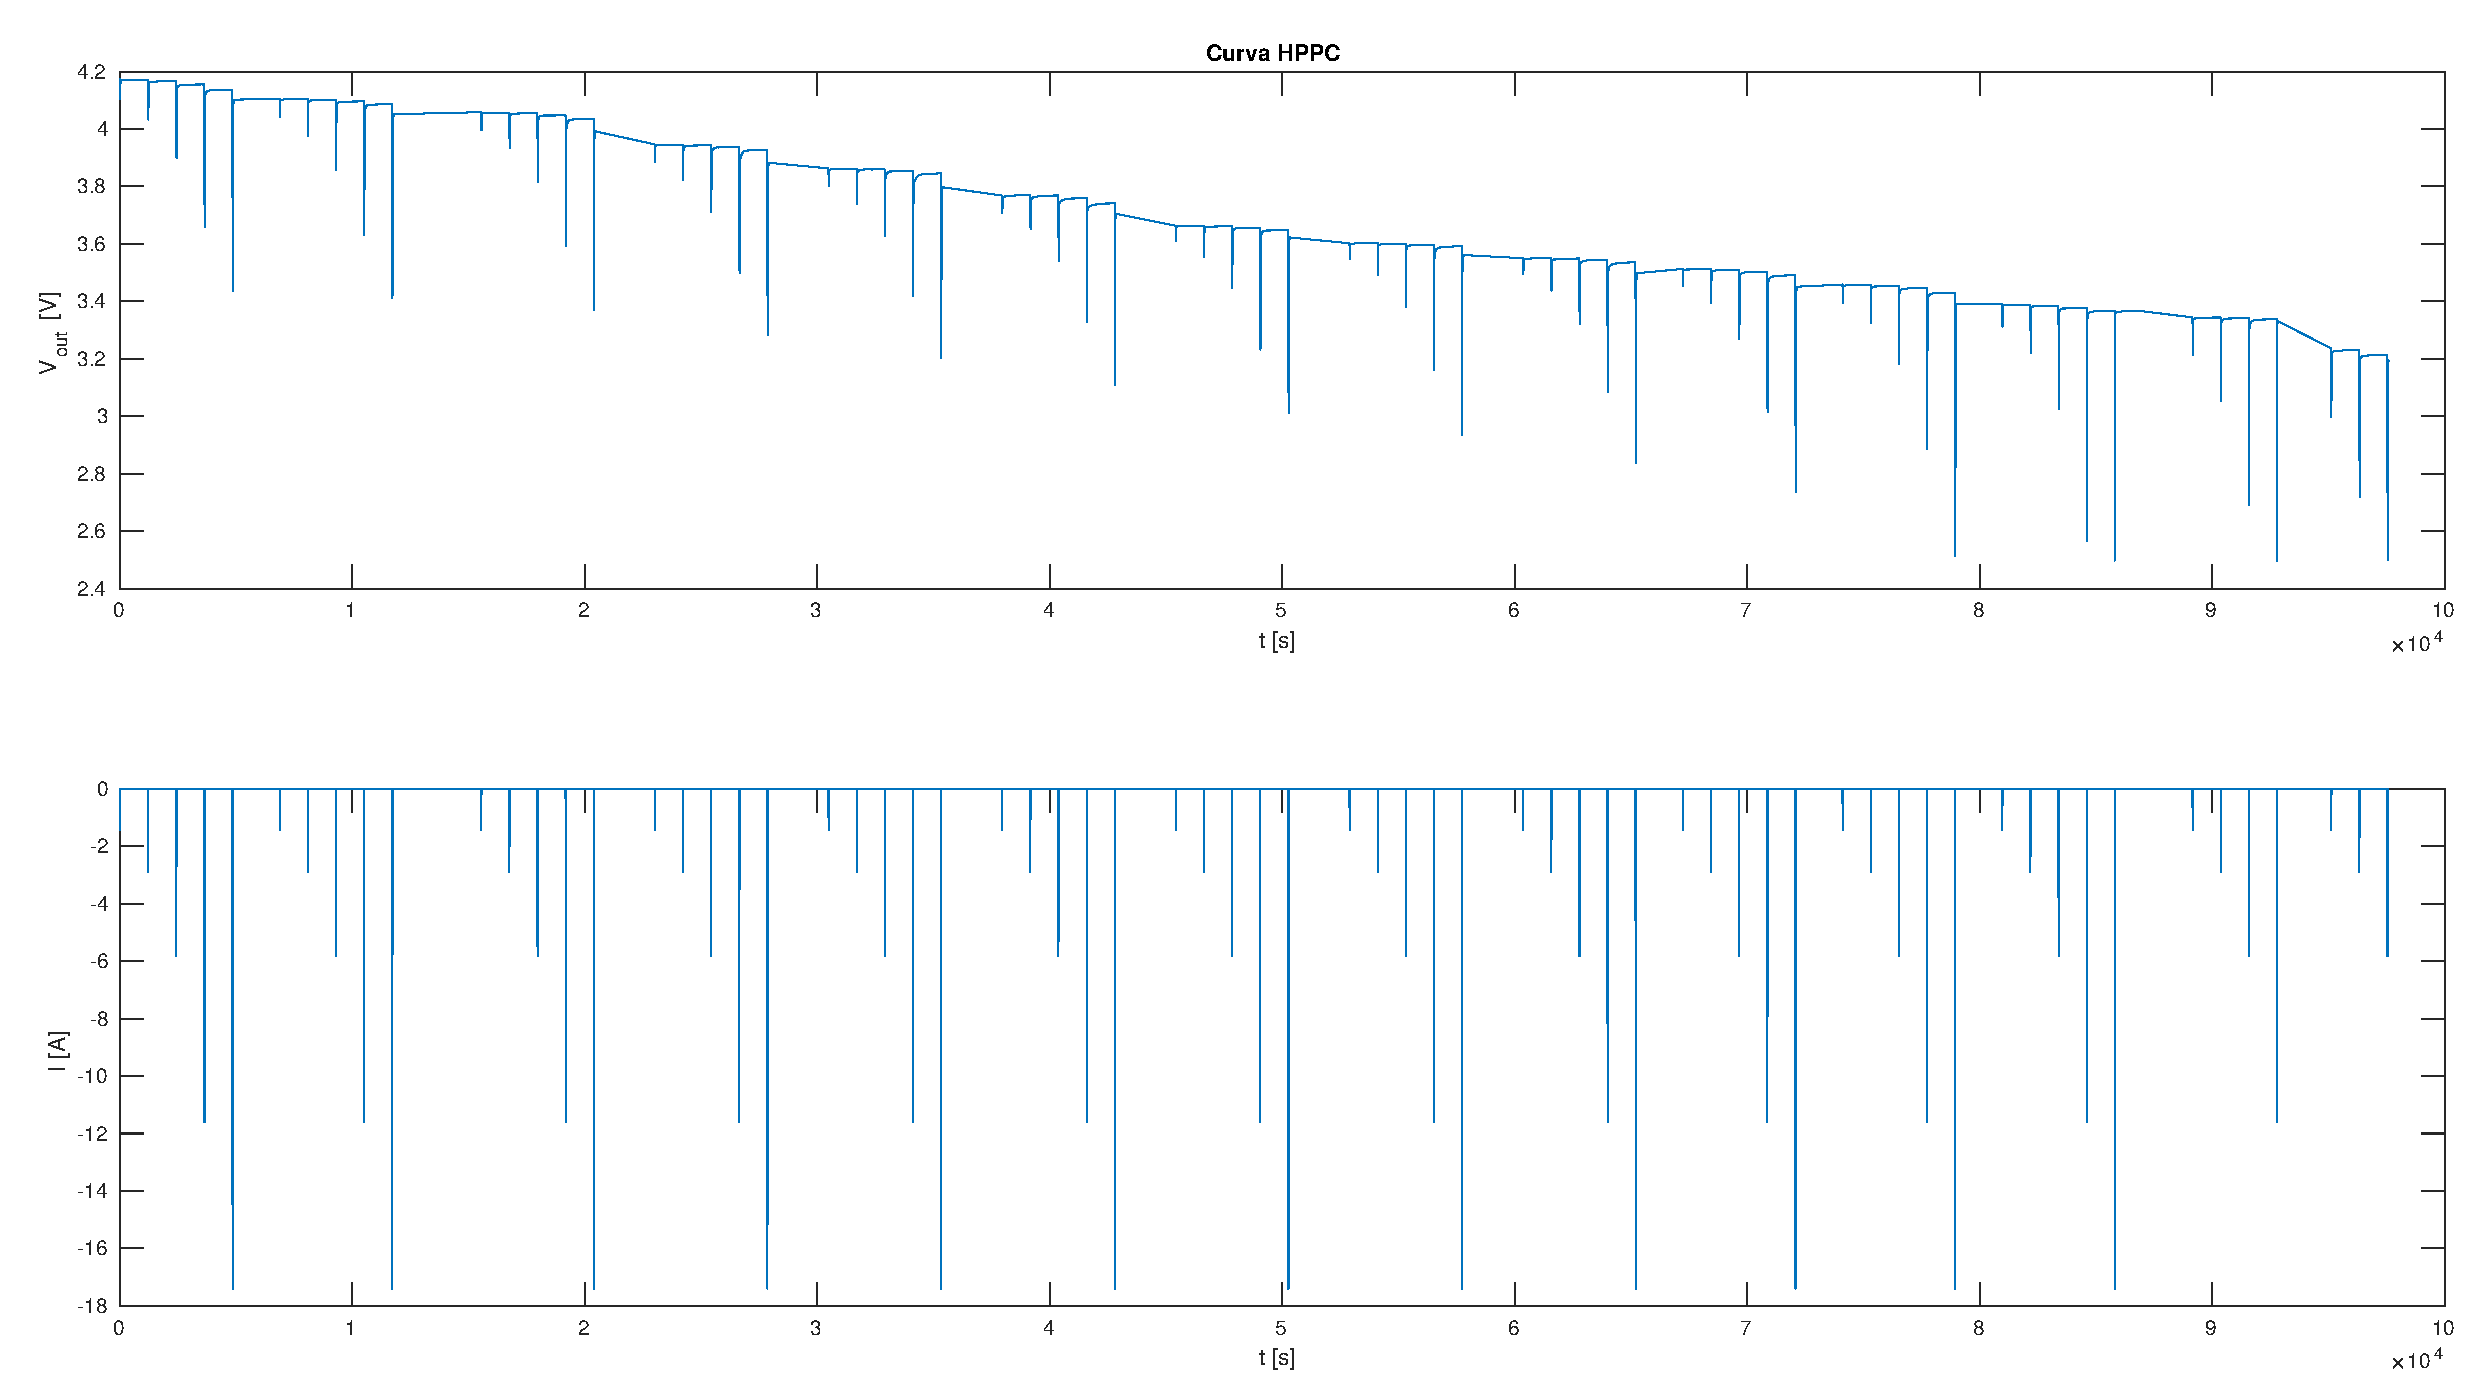
\includegraphics[width=.9\textwidth]{hppc_kollmeyer.eps}
        \caption{Curva HPPC provista por \cite{Kollmeyer2018}}
        \label{hppc_kollmeyer}
    \end{center}
\end{figure}
\FloatBarrier

%\newpage

La Figura \ref{hppc_kollmeyer_zoom} muestra una vista detallada y ampliada de
uno de los pulsos de descarga que conforman el ensayo \acrshort{HPPC}. Cada uno
de estos pulsos nos brindan no solo información respecto de la tensión de
circuito abierto (\acrshort{OCV}), sino tambien de la evolución de la celda
frente a una excitación por corriente a estados de carga (\acrshort{SOC})
determinado.

\begin{figure}[h!]
    \begin{center}
        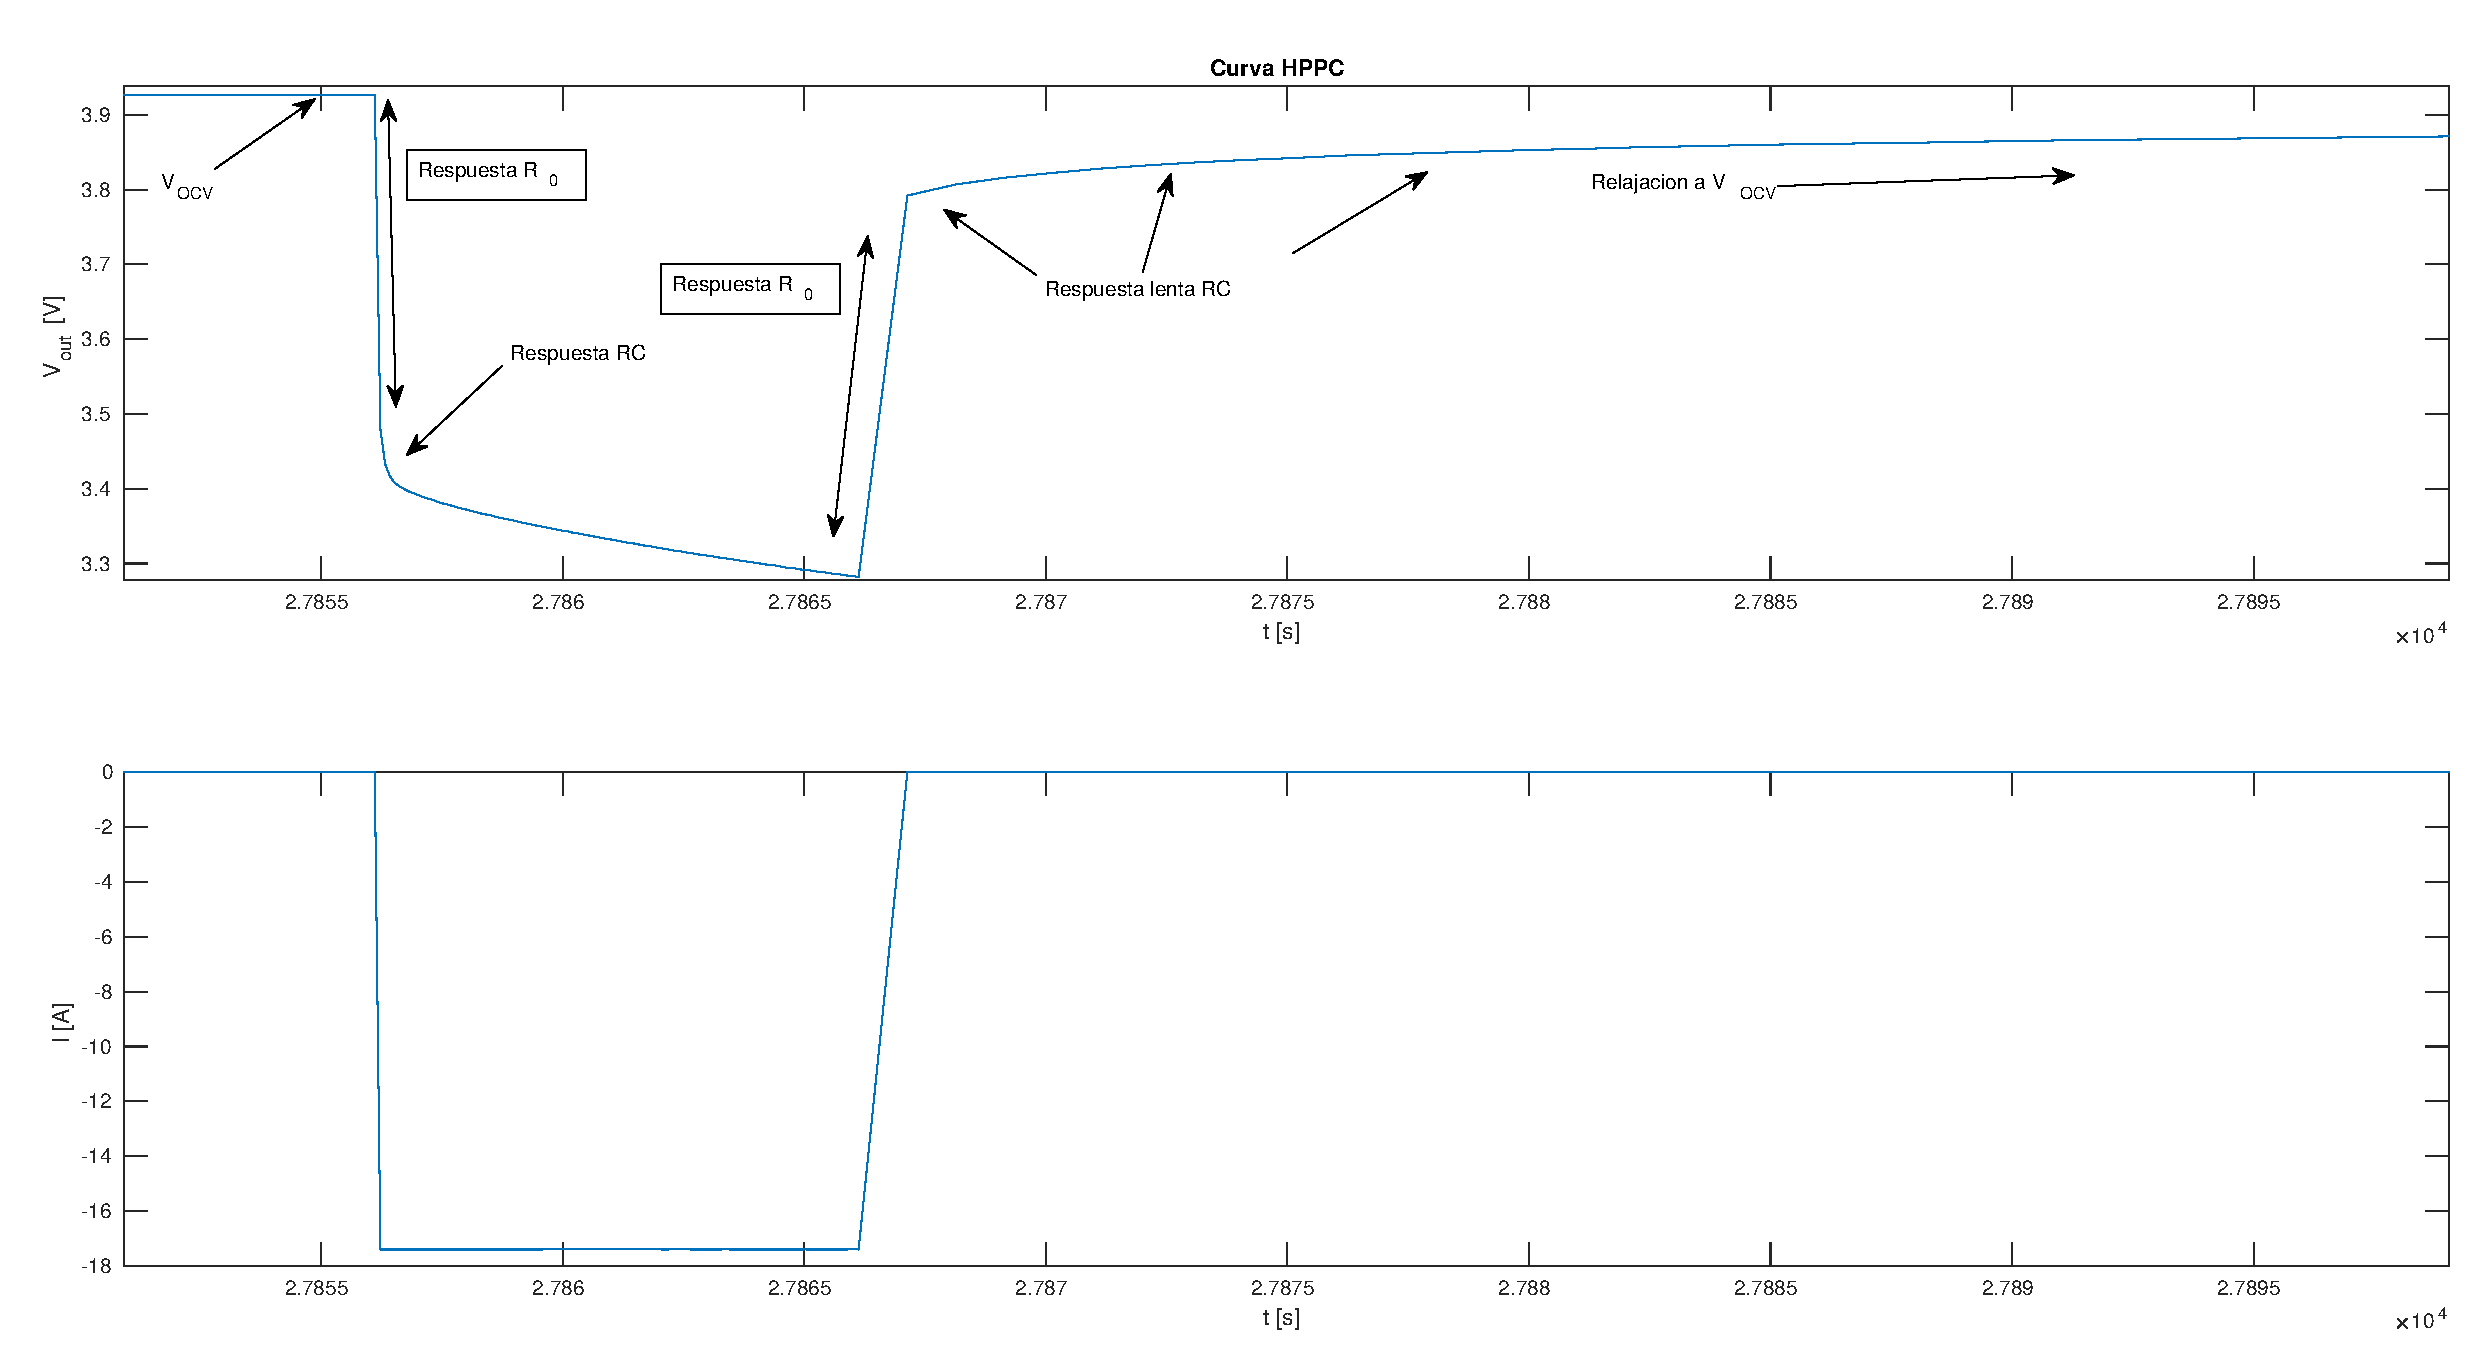
\includegraphics[width=.9\textwidth]{hppc_kollmeyer_zoom.eps}
        \caption{Ampliaci\'on sobre un pulso de la curva HPPC provista por 
                 \cite{Kollmeyer2018}}
        \label{hppc_kollmeyer_zoom}
    \end{center}
\end{figure}
\FloatBarrier

\subsubsection{Validación número de ramas R-C del modelo}

Para validar que el modelo propuesto sea capaz de describir la dinámida completa
de una celda de Ion-Litio ensayada se ajustaron 2 ecuasiones exponenciales, una
de orden 1 (Eq. \ref{eq:exp1}) y otra de orden 2 (Eq. \ref{eq:exp2}), a la curva
que traza los datos del en sayo HPPC utilizando la herramienta Curve Fitting de
Matlab.

\begin{align}
    Y &= a*exp(b*x)\label{eq:exp1}\\
    Y &= a*exp(b*x)+c*exp(d*x)\label{eq:exp2}
\end{align}

Se selecciono especificamente la fase de relajación de uno de los escalones del
ensayo HPPC. Cuando se retira el escalón de corriente, la respuesta transitoria
inmediata es condicionada por $R_{0}$ pero rapidamente la dinamica
fundamentalmente es descipta por el número de ramas R-C en serie dispuestas en
el circuito equivalente. 

\begin{figure}[h!]
    \begin{center}
        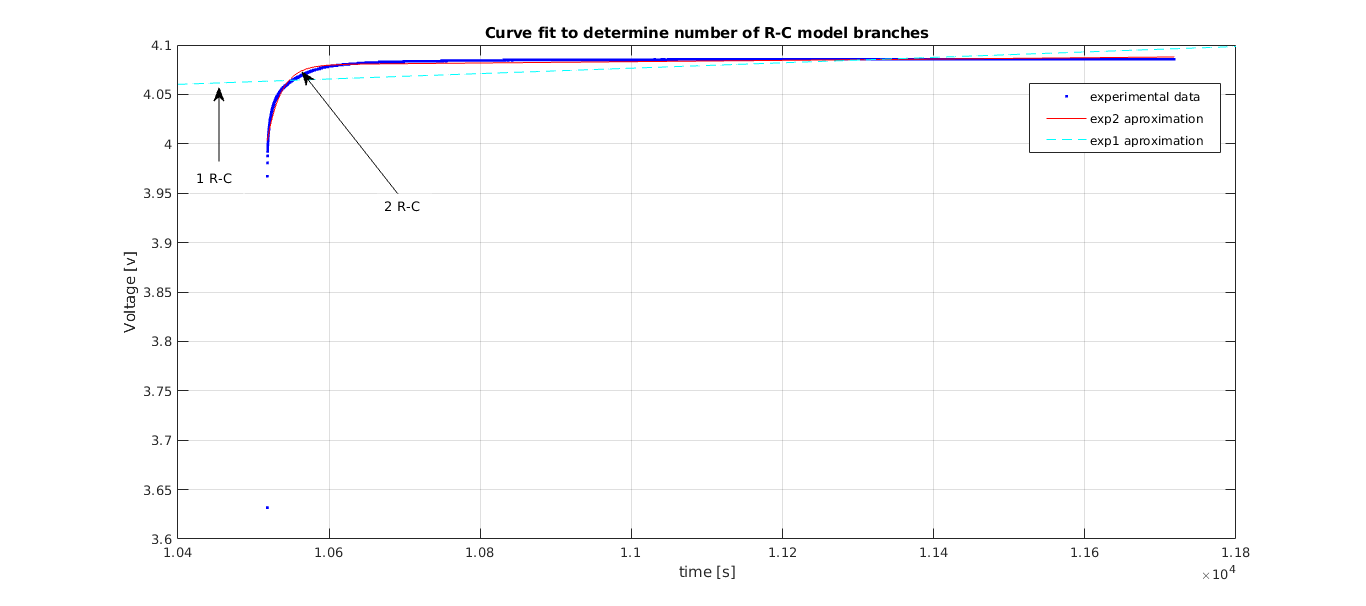
\includegraphics[width=.65\textwidth]{rc_model_fit.png}
        \caption{Ajuste curvas exponenciales orden Modelo R-C}
        \label{fig:model_fit}
    \end{center}
\end{figure}
\FloatBarrier

A la vista del resultado obtenido en la Figura \ref{fig:model_fit} se concluye
que 2 terminos exponenciales temporales serán suficientes para describir la
dinamica de una celda de Ion-Litio ensayada. Situación de compromiso entre
la precisión del modelo, la complejidad matemática y la necesidad de mantener el
costo computacional bajo a los fines de embeber el modelo en el
microcontrolador. 

\subsubsection{Implementación del circuito de Randles}

Para llevar a cabo el proceso de estimación y optimizaci\'on de par\'ametros, en
primer instancia se necesita implementar el circuito de Randles en un ambiente
de simulaci\'on. En este caso, el modelo fue desarrollado en \emph{Simulink}
utilizando la librer\'ia \emph{Power Systems} de \emph{Simscape} para crear a
medida y representar los elementos pasivos que lo componen y las señales de
entrada y salida.

El modelo est\'a compuesto por una fuente de tensi\'on controlada, que
representa el \acrshort{OCV} de la bater\'ia y 5 \acrshort{LUT}s que
representan los componentes pasivos del circuito. Los 6 componentes depende
exclusivamente del nivel de \acrshort{SOC} de la bater\'ia. Su implementaci\'on
se puede observar en la Figura \ref{battery_model_simulink}. 

El modelo implementado, a su vez, incluye una fuente de corriente a la salida
que hace las veces de carga de la celda y logra capturar la señal de corriente
proveniente del set de datos.

\begin{figure}[h!]
    \begin{center}
        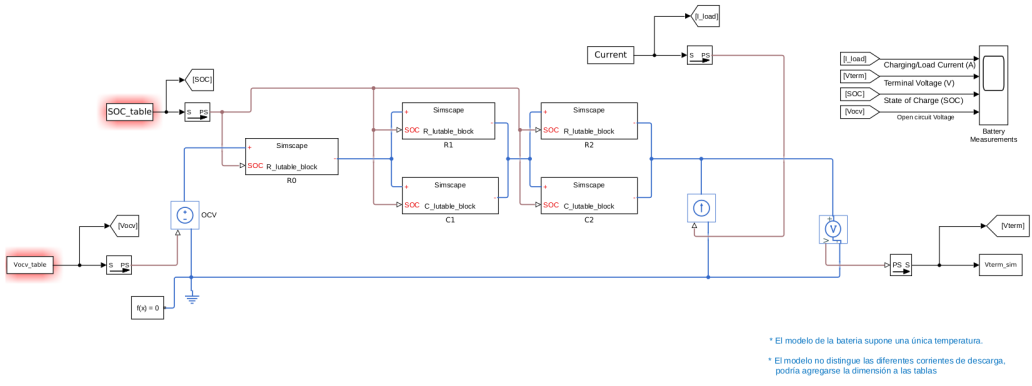
\includegraphics[width=.9\textwidth]{battery_model_simulink.png}
        \caption{Implementaci\'on del modelo de Randles en \emph{Simulink}.}
        \label{battery_model_simulink}
    \end{center}
\end{figure}
\FloatBarrier

Las variables de entrada del modelo serán entonces: 

\begin{itemize}
    \item $SOC(t)$
    \item $V_{OCV}(SOC)$
    \item $I_{load}(t)$
\end{itemize}

El modelo nos permite observar la evolucíon de la tensión en bornes de la celda
ante las variaciones de sus variables de entrada a partir de la medición de la
tensi\'on de salida que simula el mismo.

El modelado de los componentes a partir de \acrshort{LUT} no contempla
variaciones de temperatura del electrolito de la celda ni de la corriente
circulante por los elementos. Como condición de diseño se supone que el valor de
los elementos posivos no se ve modificado ante la variación de la corriente de
excitación de los mismo. Diferentes condiciones de operación, tanto en
temperatura como en corriente de excitación, requeriran simplemente repetir el
proceso de simulación para cada particularidad poblándose las nuevas dimensiones
obtenidas de la \acrshort{LUT} de forma manual.

Se valida el funcionamiento de la implementación del modelo propuesto para
representar el set de datos disponible observando la respuesta del mismo ante la
excitacipon con un escal\'on de corriente.

\newpage

Para el ensayo se utilizan par\'ametros con valores predeterminados: 

\begin{itemize}
    \item $C_{1} = C_{2} = 1F$
    \item $ R_{1} = R_{2} = 1m\mathrm{\Omega}$
    \item $\mathrm{R_0}=40m\mathrm{\Omega}$
\end{itemize}

\begin{figure}[h!]
    \begin{center}
        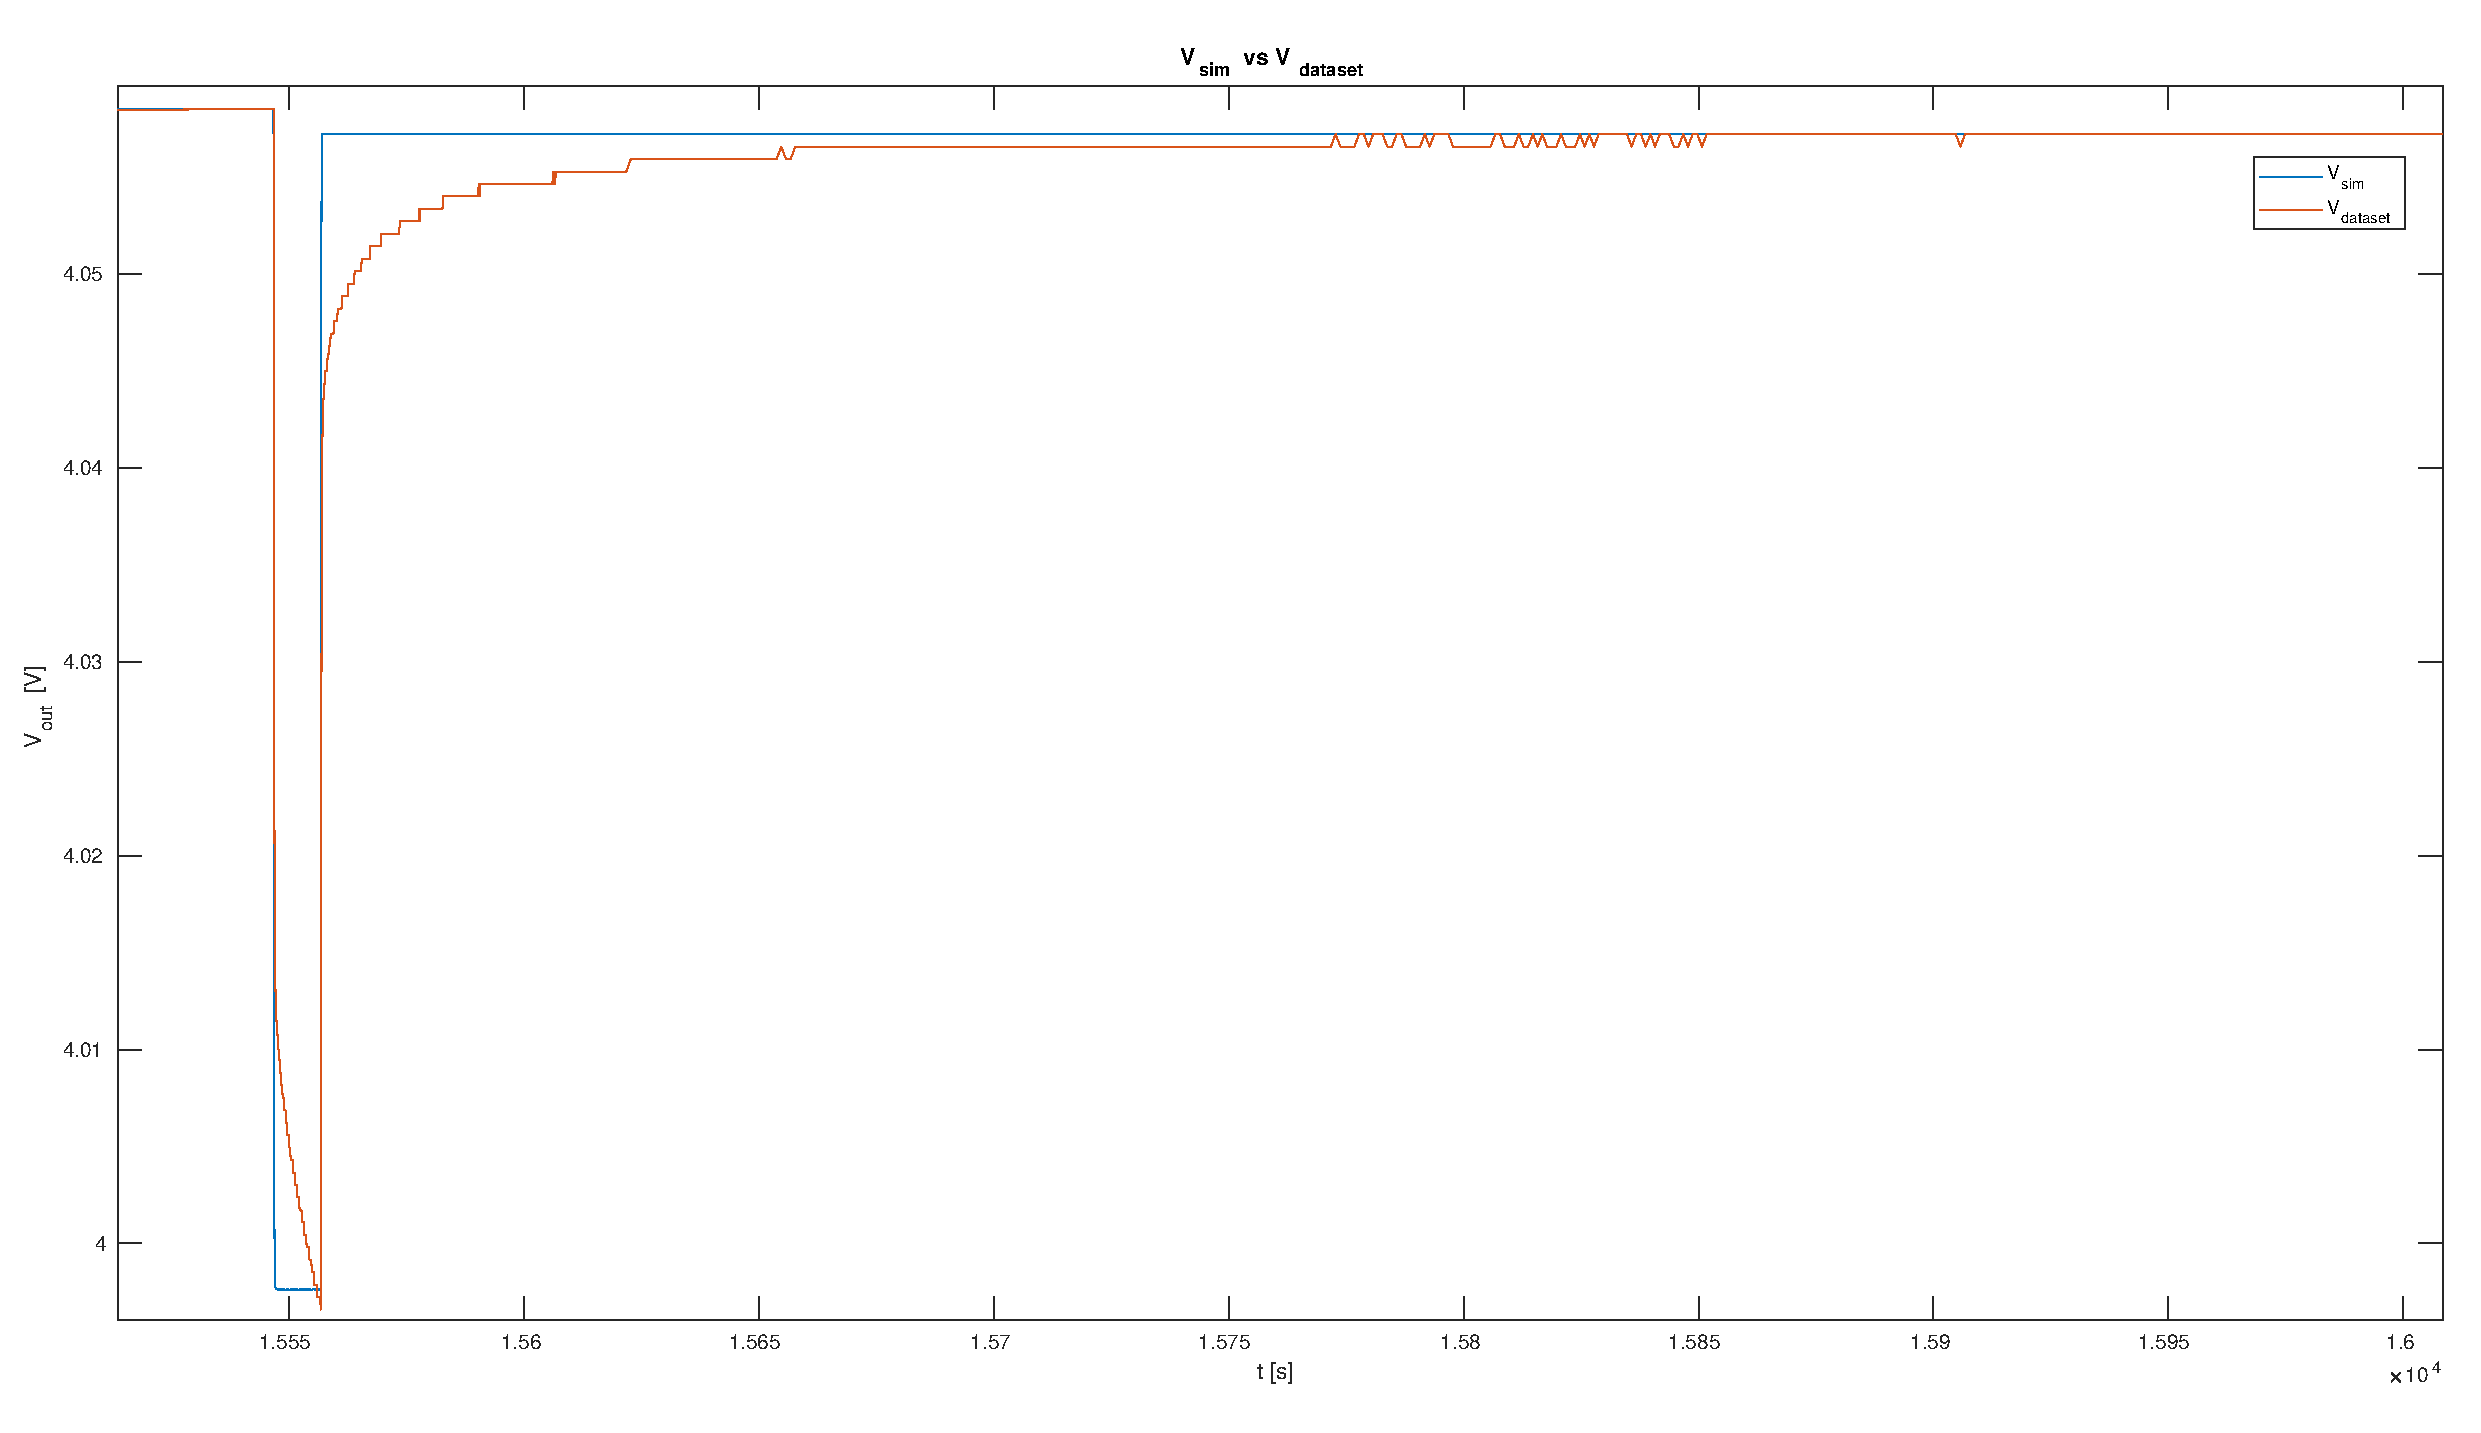
\includegraphics[width=0.8\textwidth]{v_sim_v_dataset_no_opt.eps}
        \caption{Comparaci\'on de la tensi\'on de salida del modelo de
                 \emph{Simulink} sin optimizar con la curva de tensi\'on de 
                 salida del set de datos}
         \label{comp_simulink_no_opt}
    \end{center}
\end{figure}
%\FloatBarrier

Se puede observar en la Figura \ref{comp_simulink_no_opt} que a pesar de no
estar optimizados los parámetros para disminuir el error en la tensi\'on de
salida, el modelo logra representar, de forma lejana, la din\'amica de la
respuesta al escal\'on validando la implementación realizada.

%\newpage

\subsubsection{Pre-procesamiento datos}\label{data_preprocessing}

El conjunto de datos del ensayo \acrshort{HPPC} de \cite{Kollmeyer2018} debe ser
preprocesado para obtener ciertas variables de inter\'es, como por ejemplo, la
señal del \acrshort{SOC} de la curva relevante para comparar los resultados de
nuestro modelo, como tambi\'en la segmentaci\'on o modificaci\'on de los datos
es \'util para el desarrollo del modelo.

\subsubsubsection{Curva de \acrshort{SOC}}

Dentro de los datos de la curva \acrshort{HPPC}, el ensayo de
\cite{Kollmeyer2018} acumula la corriente que circula desde y hacia el pack en
Ampehere-hora (Ah), en base a esto, se calcula \acrshort{SOC} en todo el ensayo
usando la Ecuaci\'on \ref{calculo_soc_ah}.

\begin{equation}
    SOC = \frac{Ah_{acumulado} + Ah_{min}}{Ah_{min}} \label{calculo_soc_ah}
\end{equation}

Implementando la Ecuaci\'on \ref{calculo_soc_ah} en Matlab sobre la curva Ah del
ensayo \acrshort{HPPC} se obtiene la gr\'afica que se observa en la Figura
\ref{soc_hppc_data}.

\begin{figure}[h!]
    \begin{center}
        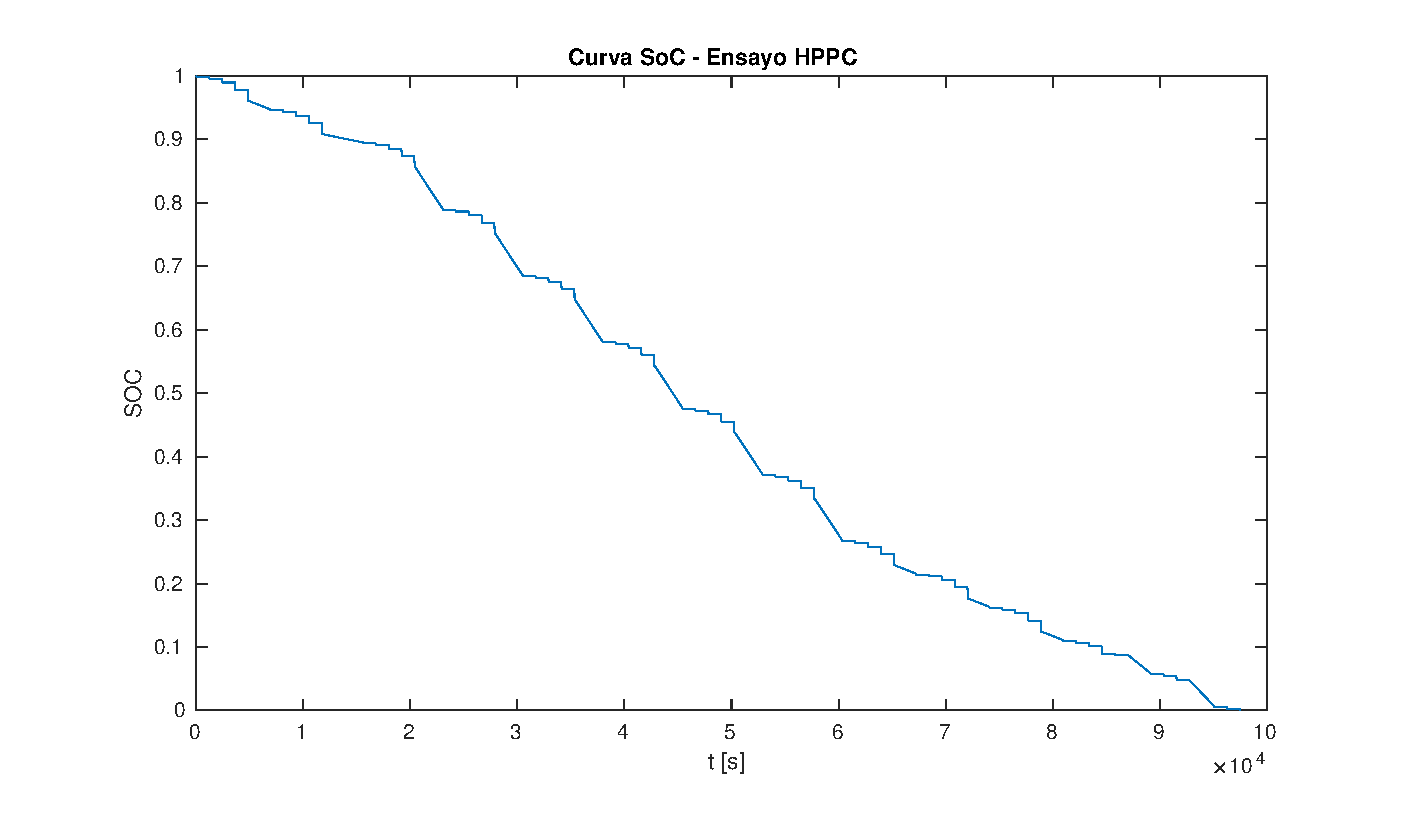
\includegraphics[width=0.8\textwidth]{soc_hppc_data.eps}
        \caption{Curva del \acrshort{SOC} para el ensayo HPPC de
        \cite{Kollmeyer2018}. En el mismo se pueden observar los escalones de
        \acrshort{SOC} generados por los pulsos de corriente aplicados en la
        celda.}
        \label{soc_hppc_data}
    \end{center}
\end{figure}
\FloatBarrier

\subsubsubsection{Obtenci\'on del \acrshort{OCV}}

Dentro de la curva \acrshort{HPPC} de la Figura \ref{hppc_kollmeyer}, podemos
observar per\'iodos de descanso lo suficientemente largos como para considerar
que la bater\'ia alcanz\'o la estabilidad qu\'imica, por lo tanto, presentando
una lectura de voltaje equivalente al \acrshort{OCV}. Esta informaci\'on del 
\acrshort{OCV} durante el ensayo, permite relacionar la tensi\'on de circuito 
abierto de la celda con el estado de carga para los distintos pulsos de la 
curva. \'Esta variable resulta de gran importancia para parametrizar y ajustar
los distintos par\'ametros del modelo, porque representa la fuente de voltaje
controlada por el \acrshort{SOC} de la Figura \ref{randles_2rc}.

Para construir la curva de \acrshort{OCV}, se retuvieron los valores de voltaje
en los puntos donde se detect\'o un flanco negativo, como se describe en la
Secci\'on \ref{flank_seg} y se extrapoló este valor hasta el siguiente flanco
negativo, obteniendo la curva de la Figura \ref{fig:ocv_detection}.

\begin{figure}[h!]
    \begin{center}
        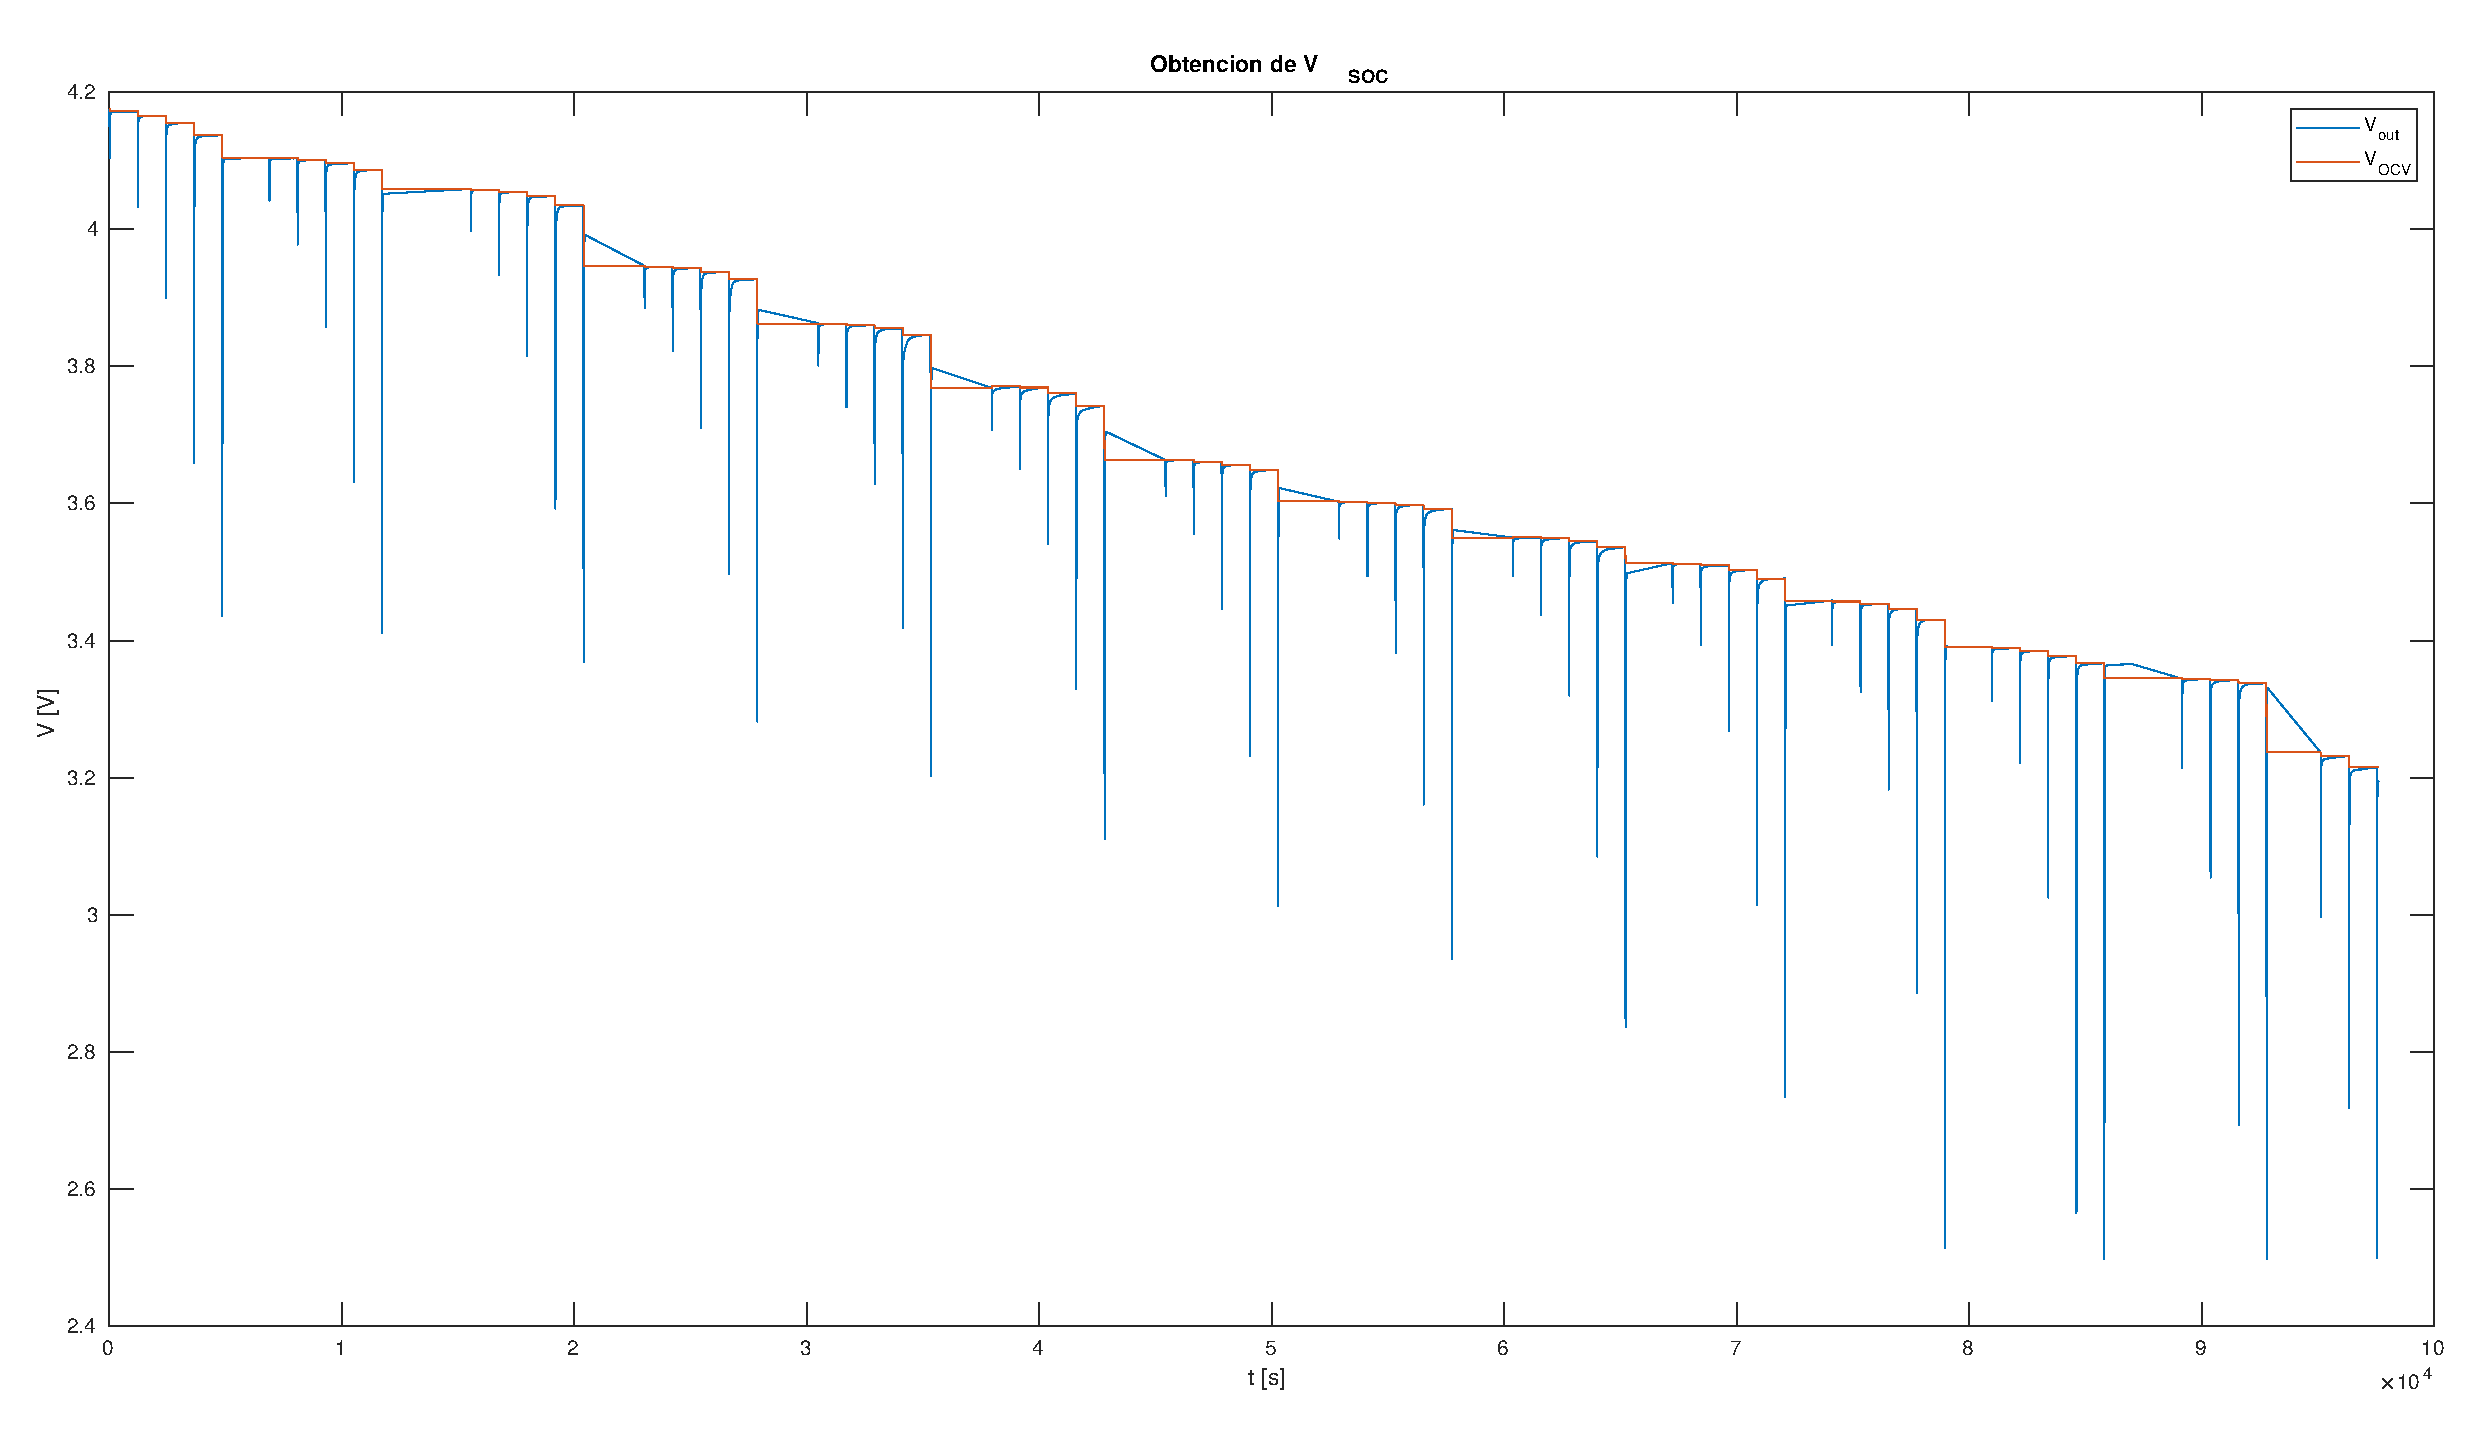
\includegraphics[width=.7\textwidth]{soc_detection}
        \caption{En naranja se muestra el \acrshort{OCV} en la que se observa
        que toma el mismo valor de voltaje antes de que ocurra el flanco
        negativo en la celda, y en azul la curva \acrshort{HPPC} original}
    \end{center}
        \label{fig:ocv_detection}
\end{figure}
\FloatBarrier

\newpage

Relacionando estos resultados con los datos obtenidos en la Figura 
\ref{soc_hppc_data}, obtenemos la curva que representa la fuente de voltaje
controlada por \acrshort{OCV} del esquem\'atico en la Figura \ref{randles_2rc}.
Esta curva se puede observar en la Figura \ref{fig:ocv_vs_soc}.

\begin{figure}[h!]
    \begin{center}
        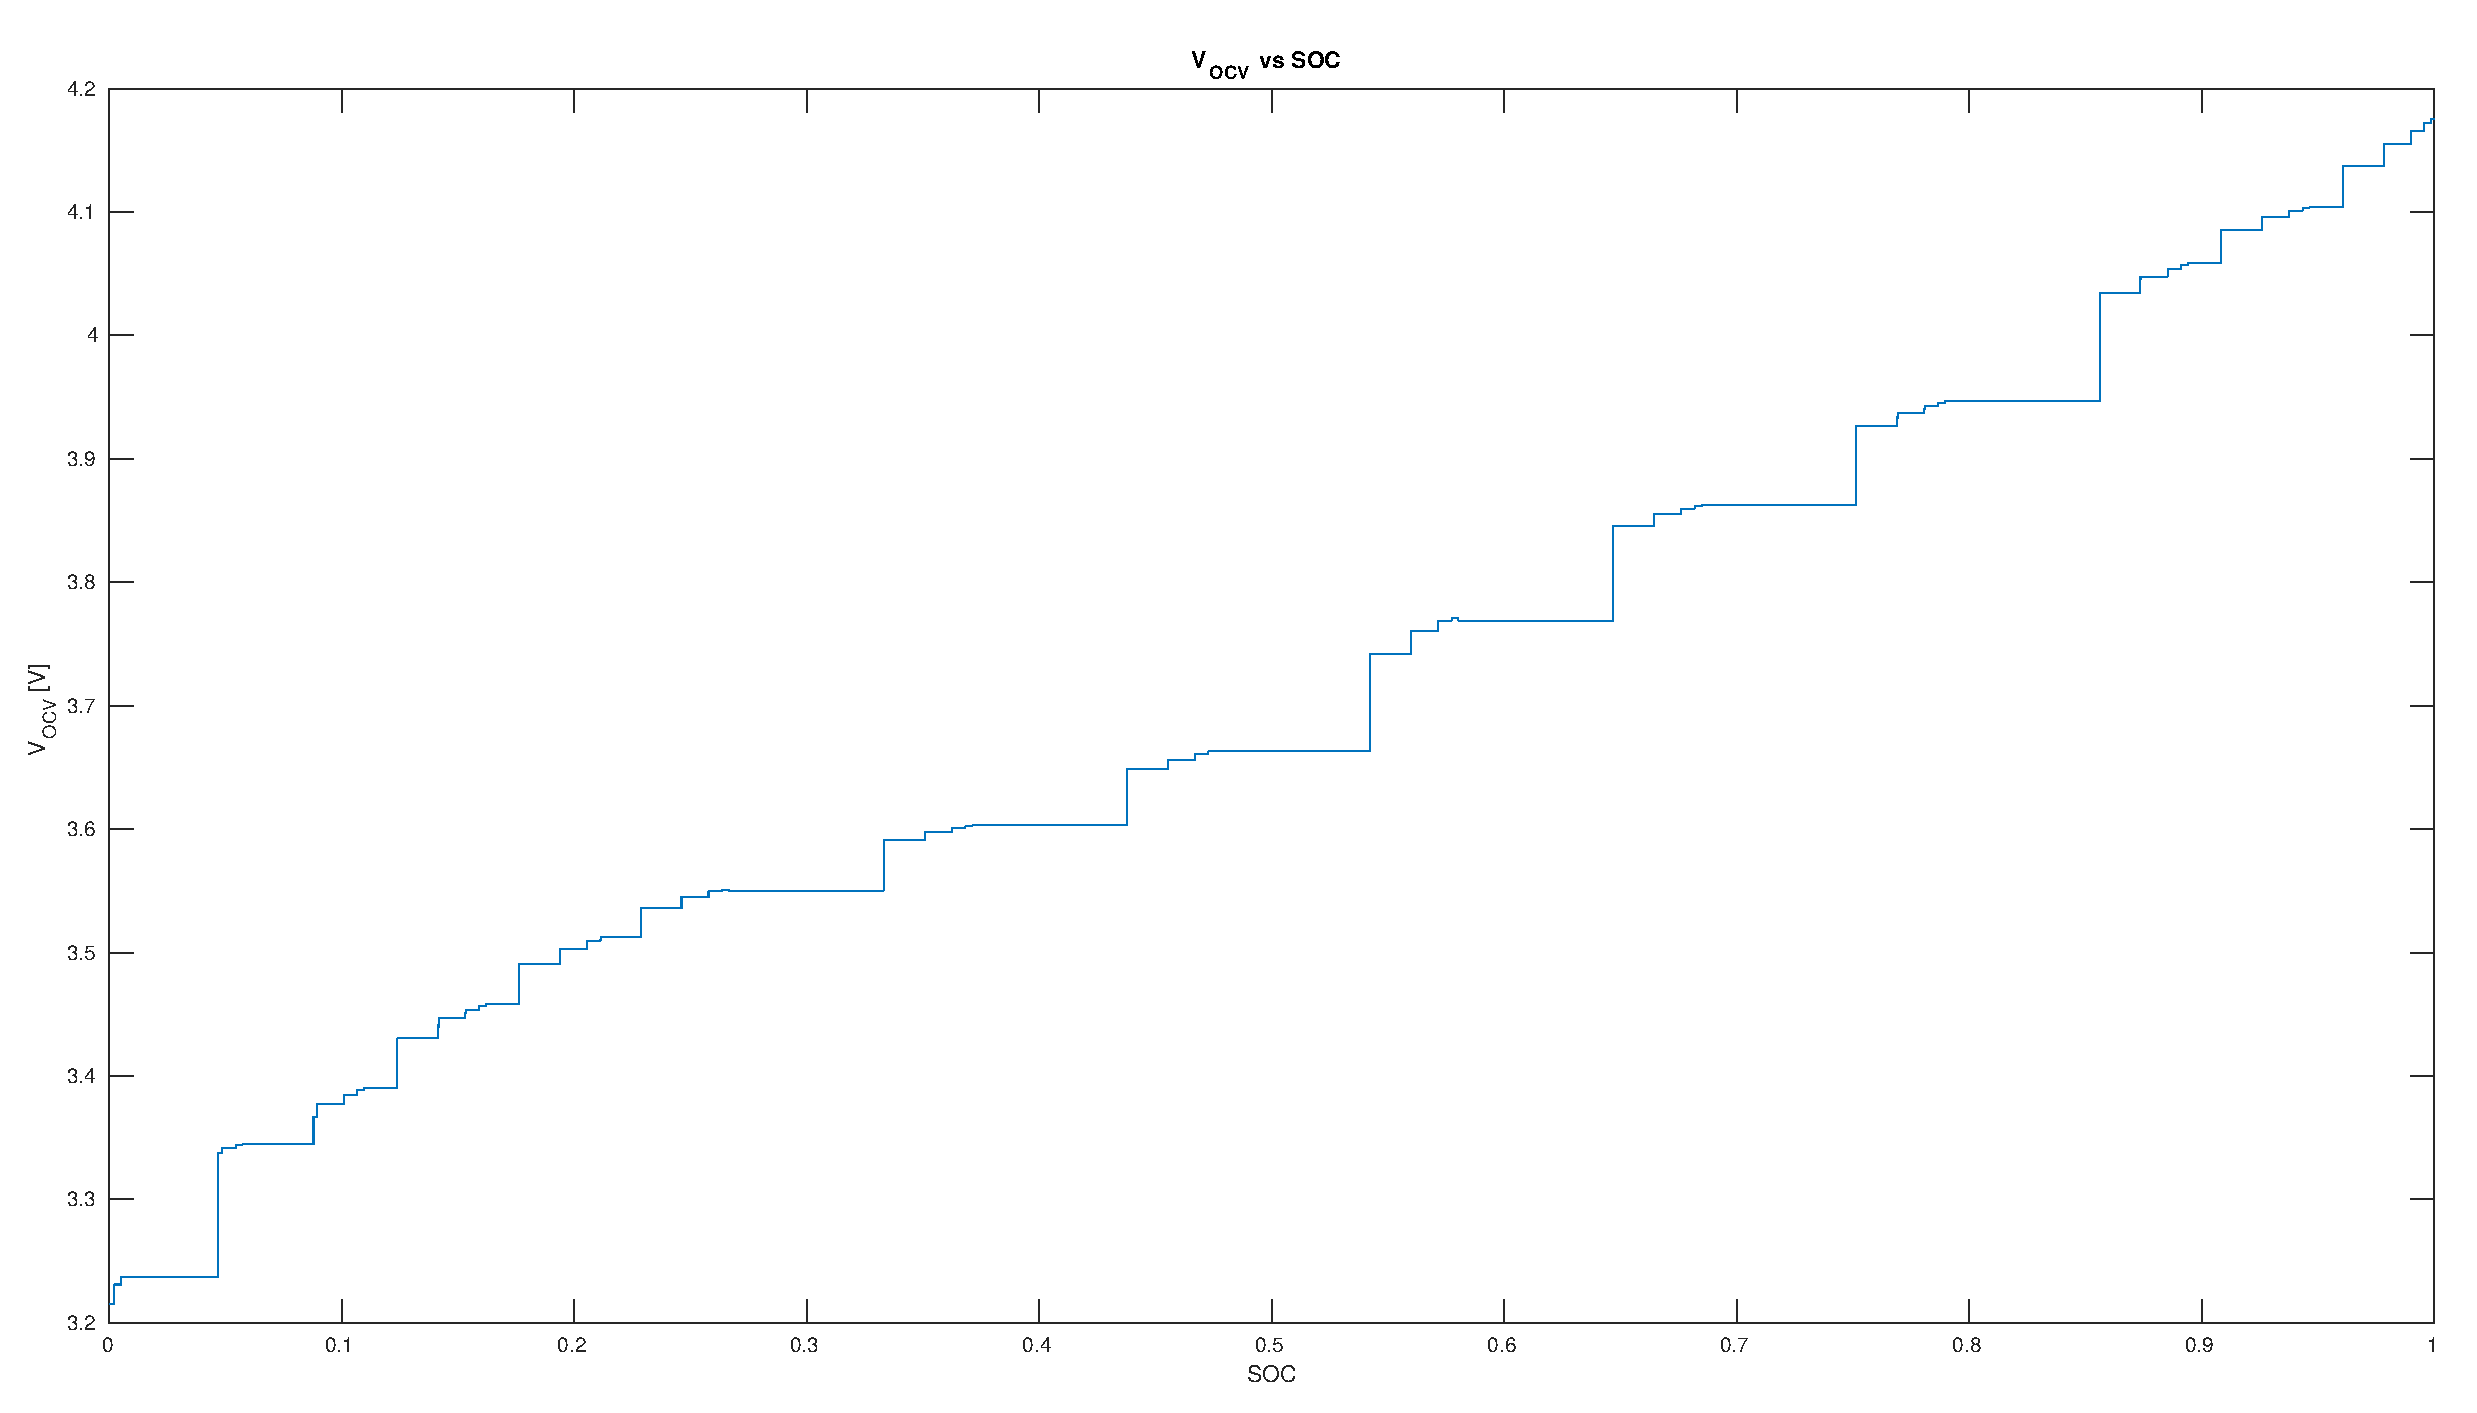
\includegraphics[width=.7\textwidth]{ocv_vs_soc.eps}
        \caption{Curva \acrshort{OCV} en relaci\'on al \acrshort{SOC}, que
            representa el funcionamiento de la fuente de voltaje controlada por
        \acrshort{SOC} en el esquem\'atico de Randles.}
    \end{center}
    \label{fig:ocv_vs_soc}
\end{figure}
\FloatBarrier

\subsubsubsection{Segmentaci\'on de Datos}\label{flank_seg}

El número de tanques R-C que conforman el modelo y consecuentemente el de
parametros a estimar, unos 67 juegos de 5 parámetros cada uno, junto con el
tamaño del dataset del ensayo \acrshort{HPPC} que se observa en la Figura
\ref{hppc_kollmeyer} plantean el desafío computacional que significa la
estimación y optimización de los mismos. 

Son parámetros a tener en cuenta la velocidad de cómputo y el consumo de
memoria, la selección de las condiciones iniciales, seteos y condiciones de
borde de los parámetros a calcular que implican una etapa de
prueva y error hasta obtener un proceso funcional acorde a los resultados
deseados y el tiempo de programación que ello implica.

Como resultado de las complejidades planteadas y en vista de evaluar el resultado
del proceso de optimizaci\'on del modelo en toda la extensión de la curva
\acrshort{HPPC}, es necesario segmentar los datos disponibles en porciones que
sean faciles de abordar. Idealmente los datos del ensayo fueron separados según
los pulsos de corriente para cada nivel del \acrshort{SOC}. 

Para ello se implementa en MATLAB un algoritmo llamado \texttt{flanks.m}, el cual
dado un arreglo de valores y un porcentaje espec\'ifico compara las muestras
entre dos instantes contiguos [n, n+1]. Si la diferencia entre ambas muestras es
mayor al porcentaje especificado de un flanco ascendente marca ese instante con
un 1, si es mayor al porcentaje anterior de un flanco descendiente marca ese
instante con -1, caso contrario, marca ese instance con un 0. Esto permite
identificar los instantes de tiempo en los que se genera un pulso de
corriente/tensi\'on de la bater\'ia para poder segmentar el conjunto de datos y
post-procesarlo para optimizar el modelo. Las \acrshort{LUT}s tendrán los saltos
en los mismos intervalos.

El resultado del algoritmo se puede observar a partir de uno de los pulsos de
corriente de la curva \acrshort{HPPC} a modo de ejemplo de su funcionamiento en
la Figura \ref{flank_seg_hppc}

\begin{figure}[h!]
    \begin{center}
        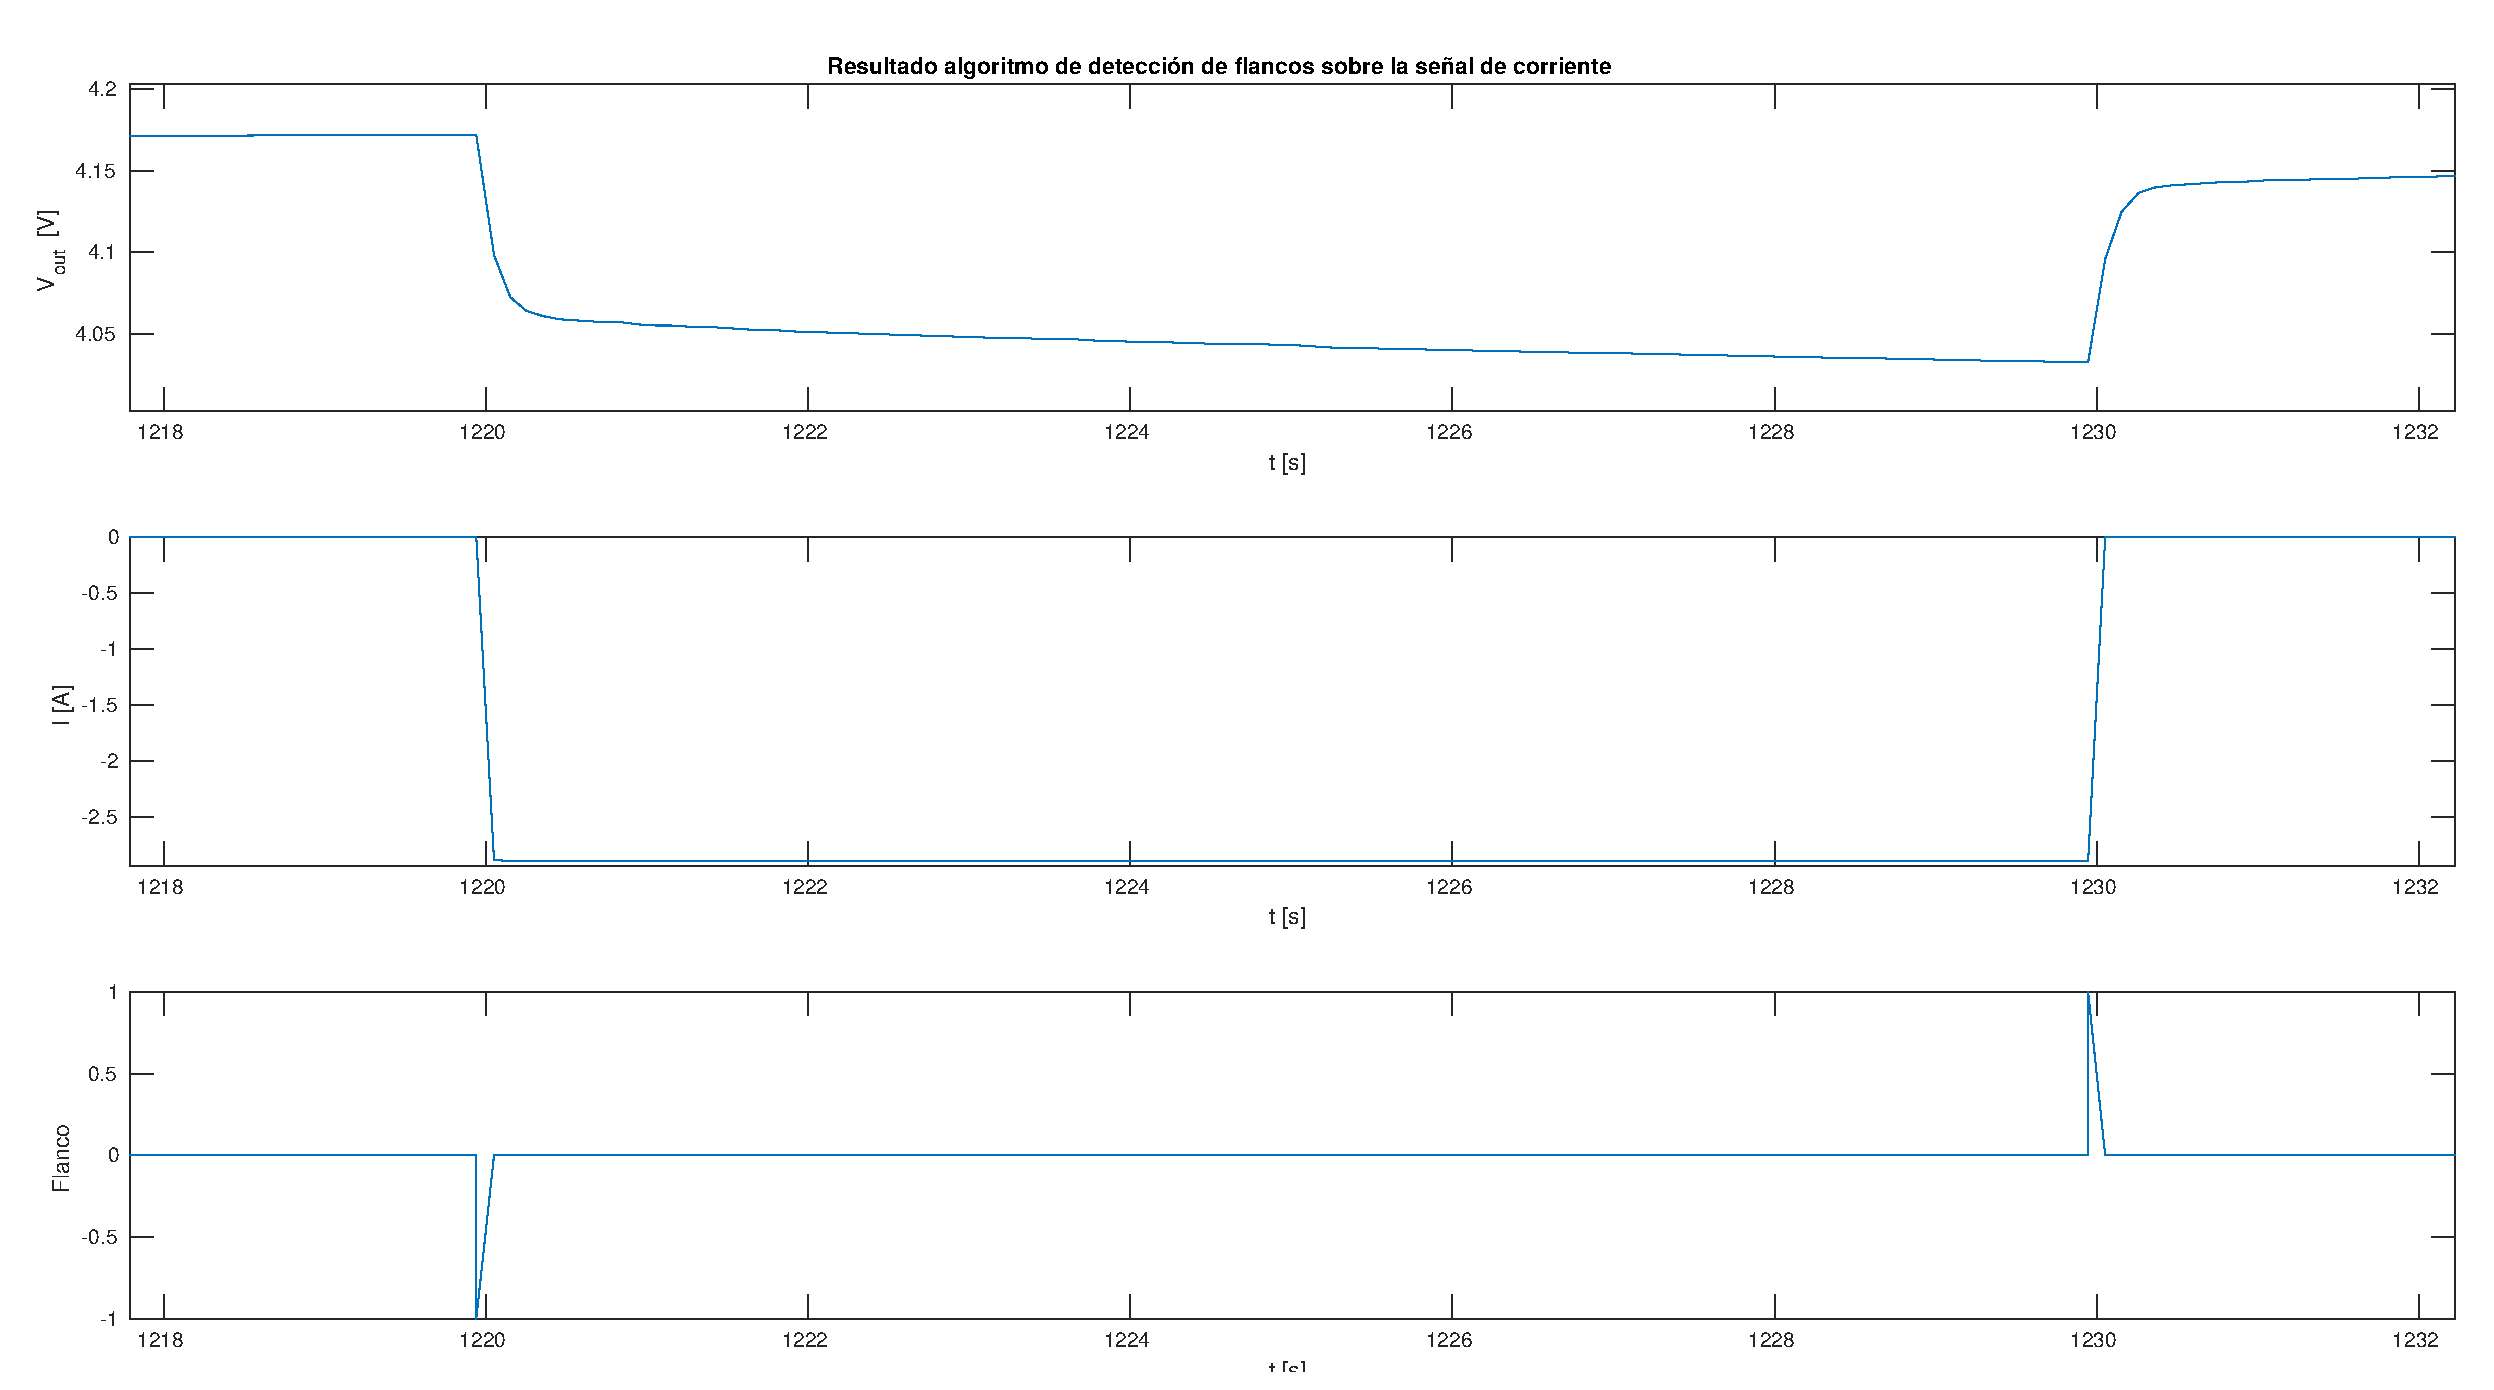
\includegraphics[width=.8\textwidth]{flank_seg_hppc.eps}
        \caption{Identificación segmentos curva
        \acrshort{HPPC}, se puede observar los picos 1 y -1 indicando los
        instantes en los que comienza y finaliza un pulso de corriente}
        \label{flank_seg_hppc}
    \end{center}
\end{figure}
\FloatBarrier

Una vez identificados todos los flancos segmentamos el set de datos en porciones
abarcables por el algoritmo de optimización. En la Imagen
\ref{fig:data_seg_hppc} se puede apreciar, a modo de ejemplo, la porción de
datos seleccionada y el criterio de corte utilizado. Para cada uno de los ciclos
de optimización se seleccionó el intervalo de datos comprendidos entre dos
flancos consecutivos descendentes. Puede notarse el solapamiento entre los
intervalos de datos seleccionados teniendo en cuenta los puntos donde se tomó el
\acrshort{SOC} para definir los cortes de la \acrshort{LUT}s. Esto permite que
el algoritmo cuente con la información suficiente para ejercitar todos y cada
uno de los parámetros del modelo.

\begin{figure}[h!]
    \centering
        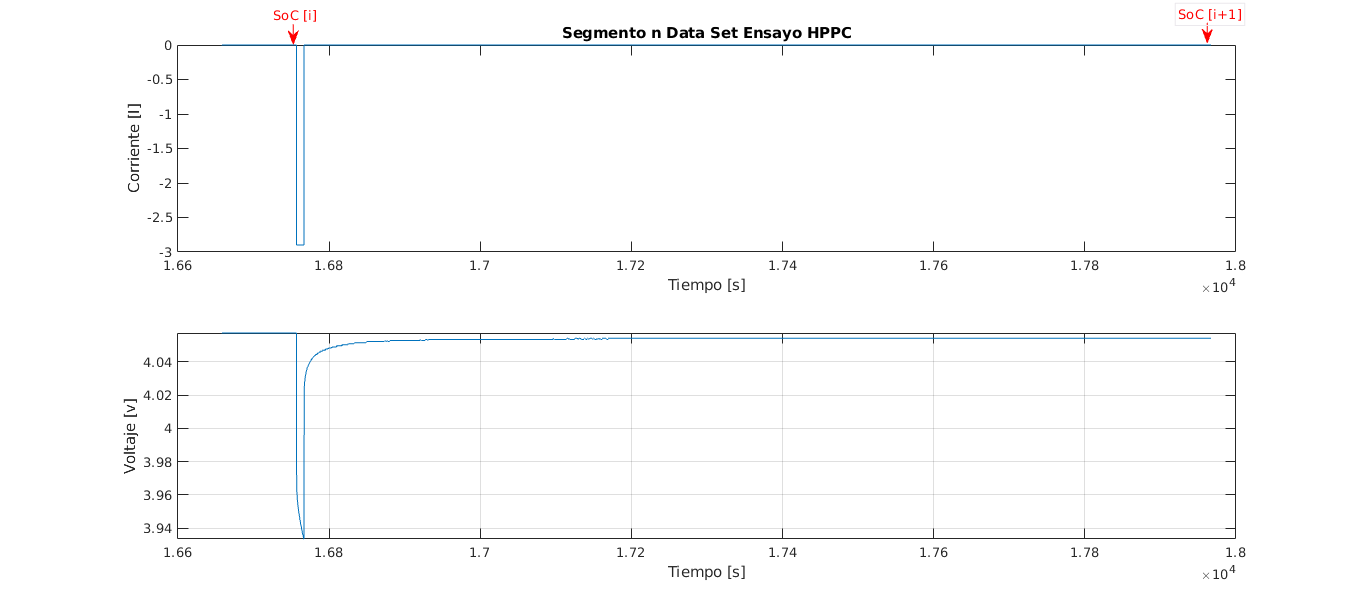
\includegraphics[width=1\textwidth]{data_seg_hppc.png}
        \caption{Segmento n - Dataset ensayo \acrshort{HPPC}}
        \label{fig:data_seg_hppc}
\end{figure}
\FloatBarrier

La posibilidad de extender o acortar los puntos de inicio y fin de la trama de
datos otorga un grado más de libertad. Dependiendo de cada ciclo de
optimización, puede ser de utilidad retener el principio del pulso siguiente
debido a que los valores de los parámetros del pulso anterior son tambien
ejercitados al principio del intervalo siguiente. 

Cada pulso de corriente y su respectiva contraparte en tensión se pueden dividir
en 2 zonas, una de excitación, aquella donde la corriente forzada está
circulando por le modelo y una zona de relajación a partir de que el pulso de
corriente es eliminado. La zona de excitación puede ser considerada como una
zona de transición entre \acrshort{SOC}s y entradas de las \acrshort{LUT}s.
Es la zona de relajación la que cuenta con la mayor información sobre de la
dinámica del sistema para ejercitar cada parámetro del modelo incluido el cambio
instantaneo de voltaje que representa $R_{0}$. La zona de excitación no 
brinda información sobre la dinámica completa del sistema, solo nos
brinda información parcial, fundamentalmente sobre la parte rápida de la
dinámica. 

\subsubsection{Algoritmo recursivo de optimizaci\'on}

El proceso de estimación y ajuste de los parámetros del modelo se realizó a
partir de la implemenación en MATLAB de un algoritmo recursivo de optimización
que ejecuta la tarea de cálculo y ajuste de cada uno de los juegos de parámetros
correspondientes a los segmentos de datos del ensayo \acrshort{HPPC} seccionados
en el pre-procesamiento de forma secuencial y automatizada.

El algoritmo desarrollado e implementado en \texttt{Semi-Automatic Li Ion
battery RC model parameters estimator.m} se repite automaticamente para cada
sección de datos seleccionada del ensayo \acrshort{HPPC} procesando cada una de
las tareas de estimación y optimización secuencialmente. El código selecciona
una porción de datos, setea los parámetros a ser estimados aplicando las
condiciones iniciales y de limites de los mismos. El codigo a su vez prepara el
modelo para ser ejecutado en cada tarea de estimación y ajuste seleccionando los
intervalos correctos de las señales de entrada del modelo y sus condiciones
iniciales.

Los límites de los parámetros a estimar se setean de forma experimental tomando
en cuentas los resultados de cálculos matematicos realizados previamente y de
algunos ciclos de optimización ejecutados a los fines de la puesta a punto del
sistema. Los valores obtenidos se definen a continuación. 

\begin{itemize}
    \item [] $ 0 < \mathbf{R_0} < 1$
    \item [] $ 0 < \mathbf{R_1} < 1$ $ 0 < \mathbf{C_1} < 200$
    \item [] $ 0 < \mathbf{R_2} < 1$ $ 0 < \mathbf{C_2} < 3000$
\end{itemize}
\FloatBarrier

Una vez que se encuentra corriendo la tarea de optimización, la implementación
ejecuta un algoritmo automatizado de optimización numérica a partir de la
herramienta de Estimación de Parametros, parte del toolbox \emph{Design
Optimization} de \emph{Simulink} que provee de funciones, herramientas activas
y bloques para el tratamiento de modelos. El toolboox provee de la capaciad de
interacción entre el modelo de la celda desarrollados con la librer\'ia
\emph{Power Systems} de \emph{Simscape}, la información experimental del ensayo
\acrshort{HPPC} proveniente del dataset y el algoritmo de optimización planteado.

El método matematico de optimización seleccionado es el de mínimos cuadrados no
lineales implementado a partir de la función \emph{lsqnonlin} del toolbox de
optimización. 
El método minimiza los cuadrados de los residuos, por lo que requiere ser
provisto de un vector de errores residuales, particular de nuestra solución, el
cual se computa sobre una base de tiempo fija.
El solucionador de mínimos cuadrados no lineales resuelve problemas de ajuste de
curva de mínimos cuadrados no lineales de la forma

\begin{equation}
    \min_{x}\|f(x)\| = \min_{x} (f_1(x)^2 + f_2(x)^2+\dots+f_n(x)^2)
\end{equation}

El vector de errores residuales se implementa en
\texttt{sdoVtermEstimation\_Objective.m}. La función es provista al optimizador y
utilizada para simular y comparar la salida obtenida del modelo respecto de los
datos experimentales provistos. Los argumentos devueltos por la función
contienen imformación respecto de como se ajustan los resultados de la
simulación $y_{s}(t)$ a los datos experimentales $y_{r}(t)$ en todos los puntos
simulados de la forma observada en la Ecuación \ref{eq:residual}.

\begin{equation}
    e(t) = y_{s}(t)–y_{r}(t) 
    \label{eq:residual}
\end{equation}

La función devuelve un vector de valores y no la suma de los cuadrados de los
valores. El algoritmo de optimización calcula implícitamente la suma de los
cuadrados de las componentes de $F(x)$ del vector de errores devuelto de la
forma vista en la Ecuación \ref{eq:residual_vect}.

\begin{equation}
    F(x) = \begin{bmatrix}
        e(0)\\
        \vdots\\
        e(N)\\
    \end{bmatrix}
    \label{eq:residual_vect}
\end{equation}

La selección del método de optimización fue realizada a instancias de
\cite{Jackey2013BatteryMP} y debido a que el método \emph{lsqnonlin} es
computacionalmente varias veces más rápido en comparación a otros metodos para
la solución del problema en cuestión.

El proceso de optimización se completa una vez que el tamaño del gradiente del
vector residual es menor que el valor de tolerancia de optimización
seleccionado.

\begin{figure}[h!]
	\begin{center}
		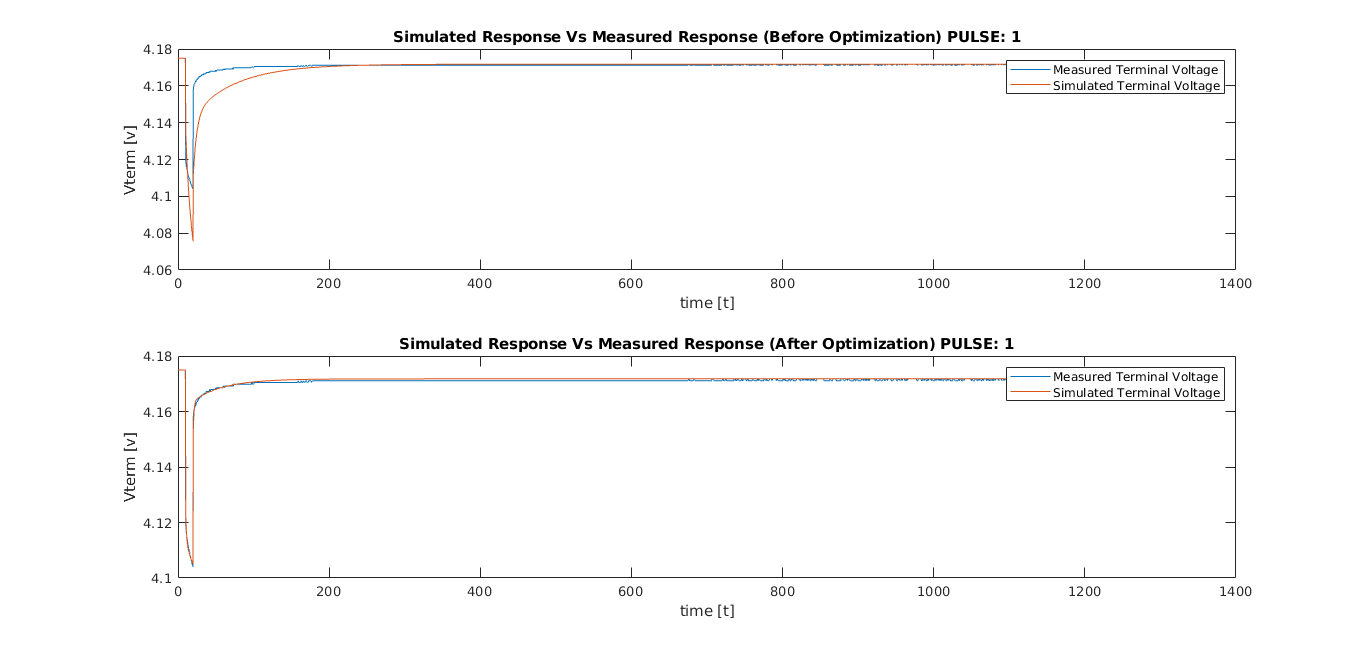
\includegraphics[width=1\textwidth]{sim_vs_measured_response.png}
		\caption{Respuesta simulada Vs Respuesta Medida antes - Resultado
        proceso de optimización}
		\label{fig:sim_vs_mea_resp}
	\end{center}
\end{figure}
%\FloatBarrier

Una vez finalizada cada tarea de optimización el algoritmo presenta la comparación gráfica de los
datos obtenidos de la slimulación respecto de los datos experimentales antes y
despues de ejecutado el proceso de optimizaciónlas, como
las de la Figura \ref{fig:sim_vs_mea_resp}. Estas gráficas sirven para
validar el proceso de optimización llevado a cabo y como mecanismo de control y
corrección de los inconvenientes que se presenten durante el proceso de cálculo
y optimización cuando los resultados simulados no converjan con los datos
experimentales.

\subsubsection{Validación de los parámetros}\label{val_param_modelo}

Los resultados finales se presentan en la Figura \ref{fig:exp_vs_sim} donde se
comparan los datos experimentales completos del ensayo \acrshort{HPPC} con los
obtenidos al simular el modelo.
Para evaluar los resultados del algoritmo de optimización y la calidad de la
simulación obtenida con cada uno de los 66 juegos de parámetros calculados fue
necesario observar puntualmente cada escalon de corriente del ensayo,
focalizándonos en aquellos donde la tensión en bornes de la simulación no logra
converger con los datos experimentales.

\begin{figure}[h!]
	\begin{center}
		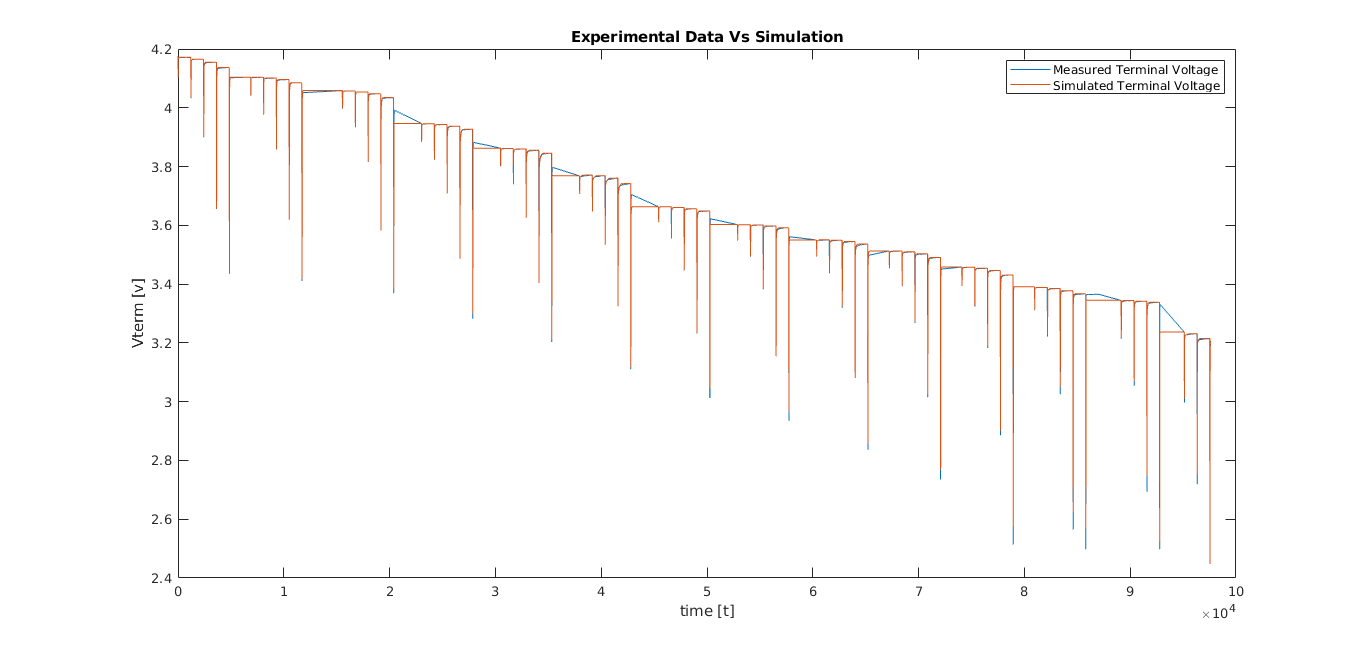
\includegraphics[width=1\textwidth]{Vterm_exp_vs_sim.png}
		\caption{Respuesta Simulada Vs Respuesta Medida}
		\label{fig:exp_vs_sim}
	\end{center}
\end{figure}

Para cada nivel de \acrshort{SOC} el ensayo aplica 5 pulsos de corriente de
descarga consecutivos, como se describe en la Sección \ref{ensayo_HPPC}. Para
cada nivel de \acrshort{SOC} la simulacióni del 5to escalón de corriente no
logra ajustarse a los datos experimentales como se observa, a modod de ejemplo,
en la Figura \ref{fig:exp_vs_sim_5_error}.

Este fenómeno se explica debido a que el dataset no incluye la información de
los periodos de descarga largos que llevan la celda al siguiente esclon de
\acrshort{SOC} de ensayo. Por lo cual, estos pulsos carecen de la información
sufuciente respecto del estado de relajación final de la celda una vez
finalizado el pulso de corriente. Por otra parte no es casualidad que el
fenómeno se precente en los pulsos de descarga de mayor intensidad, siendo los
que tienen mayor posibilidad de modificar el \acrshort{SOC} de la celda pese a
no ser la intención del ensayo.

\begin{figure}[h!]
	\begin{center}
        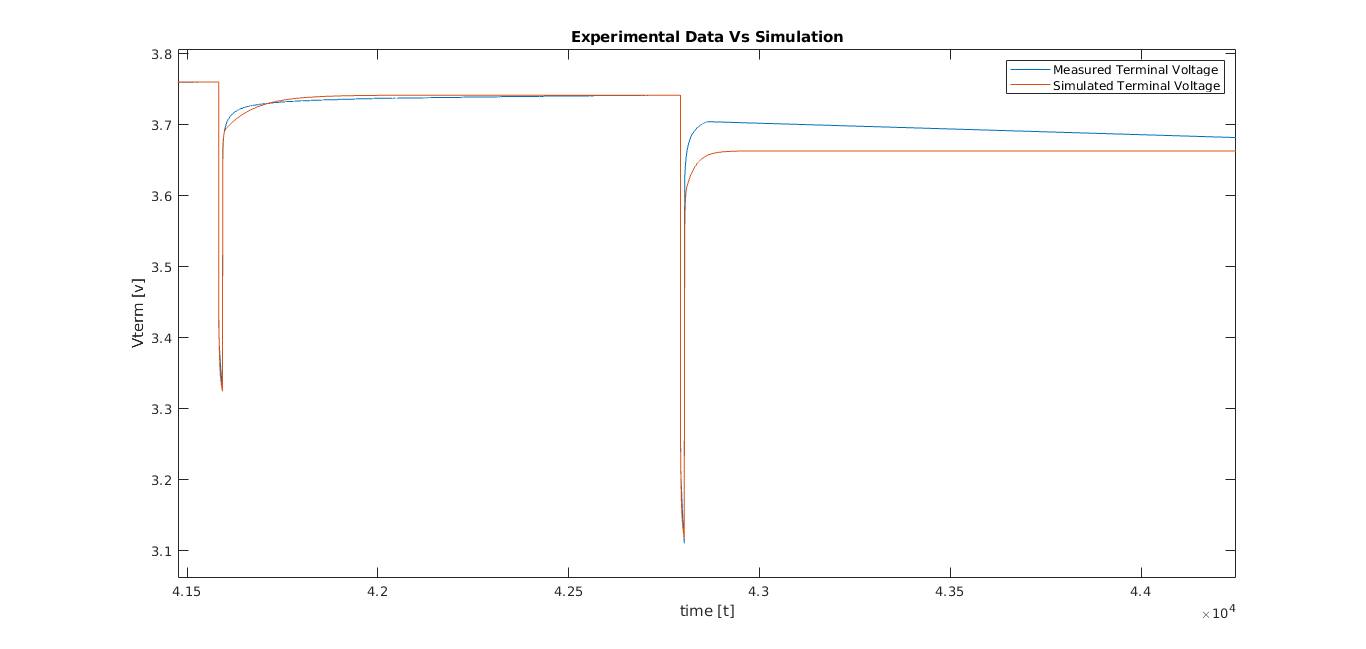
\includegraphics[width=0.8\textwidth]{Vterm_exp_vs_sim_pulse_5_error.png}
		\caption{Pulso no convergente}
		\label{fig:exp_vs_sim_5_error}
	\end{center}
\end{figure}

Viendo que el patrón se repetía sistemáticamente en los pulsos 5tos de cada uno
de los escalones de \acrshort{SOC}. Y considerando que el dataset no cuenta con
la información suficiente para ajustar los parámetros en los pulsos de ensayo en
cuestion. La solución aplicada para corregir las \acrshort{LUT}s fue la de
eliminar los juegos de parametros correspondientes a los pulsos defectuosos. Es
así que concluimos el proceso de cálculo y optimizción con 55 juegos de
parametros correspondientes a 55 \acrshort{SOC} de la celda que modelan la
dinámica completa de la misma a la temperatura del electrolito de $25\deg C$.

La Figura \ref{fig:lut_RC} pesenta los valores finales de la \acrshort{LUT}s ya
optimizadas para el cirucuito equivalente.

\begin{figure}[h!]
    \begin{center}
        \begin{subfigure}{.6\textwidth}
            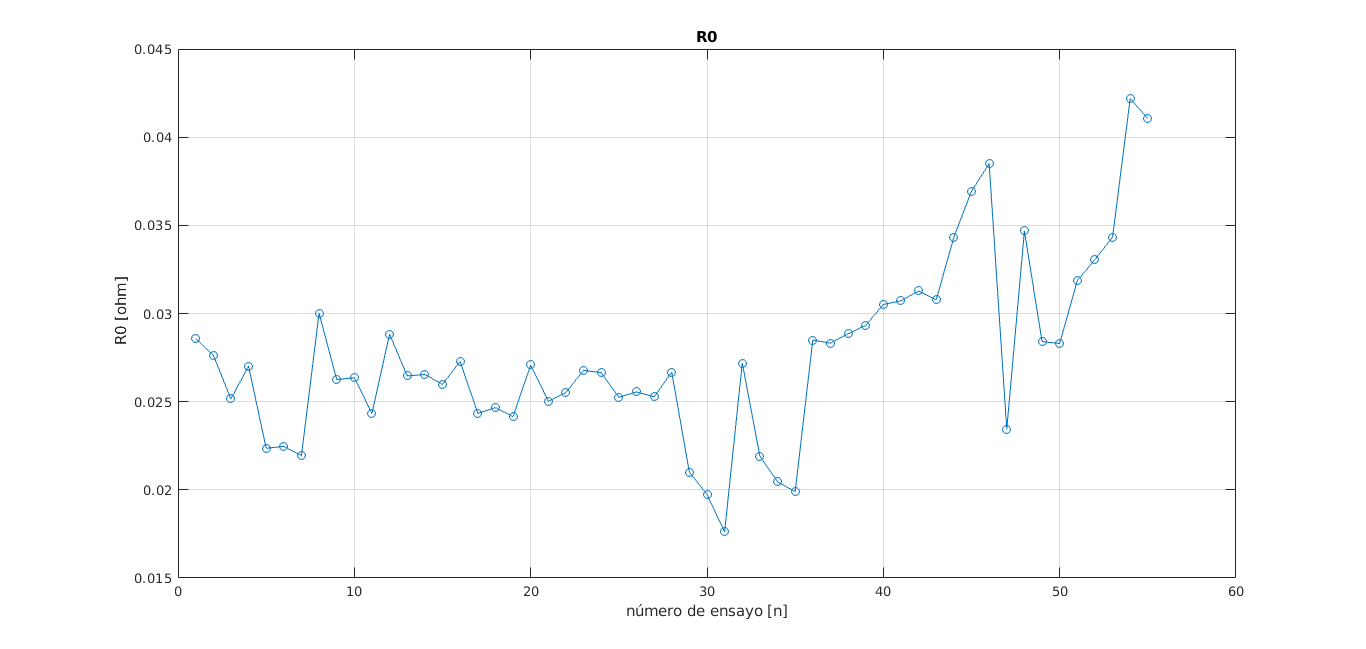
\includegraphics[width=1\textwidth]{R0_lutable_corrected.png}
            \caption{\acrshort{LUT} $R_0$}
            \label{fig:lut_R0}
        \end{subfigure}
        \begin{subfigure}{1\textwidth}
            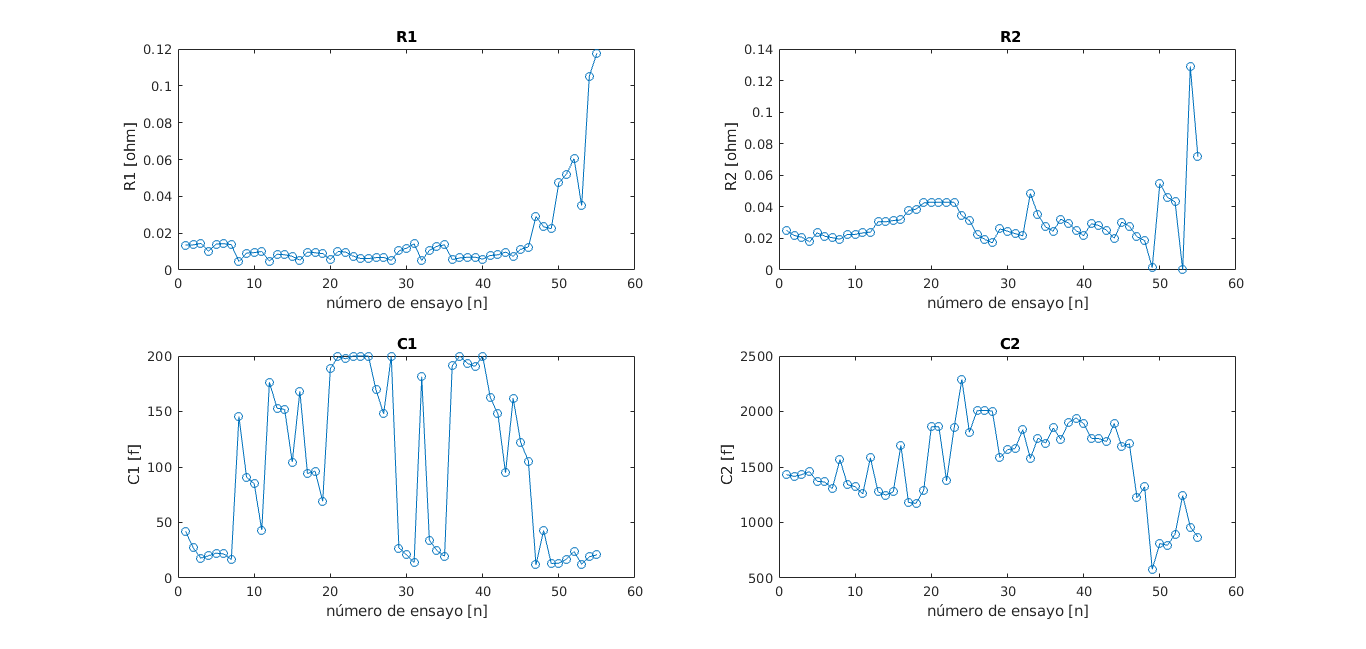
\includegraphics[width=1\textwidth]{RC_lutables_corrected.png}
            \caption{\acrshort{LUT}s $R_1$, $C_1$, $R_2$, $C_2$}
            \label{fig:lut_RCn}
        \end{subfigure}
    \end{center}
    \caption{Valores finales R y C \acrlong{LUT}s}
    \label{fig:lut_RC}
\end{figure}
\FloatBarrier

Validamos los juegos de parámetros finales corregidos sometiendo el modelo
calculado a multiples perfiles de corriente de distintos drive cicles y
comparando los datos obtenidos con los valores experimentales. En la Figura
\ref{fig:DC_modVsData} se se puede apreciar que la simulación del drive cicle
coincide con los datos experimentales.

\begin{figure}[!h]
    \centering
    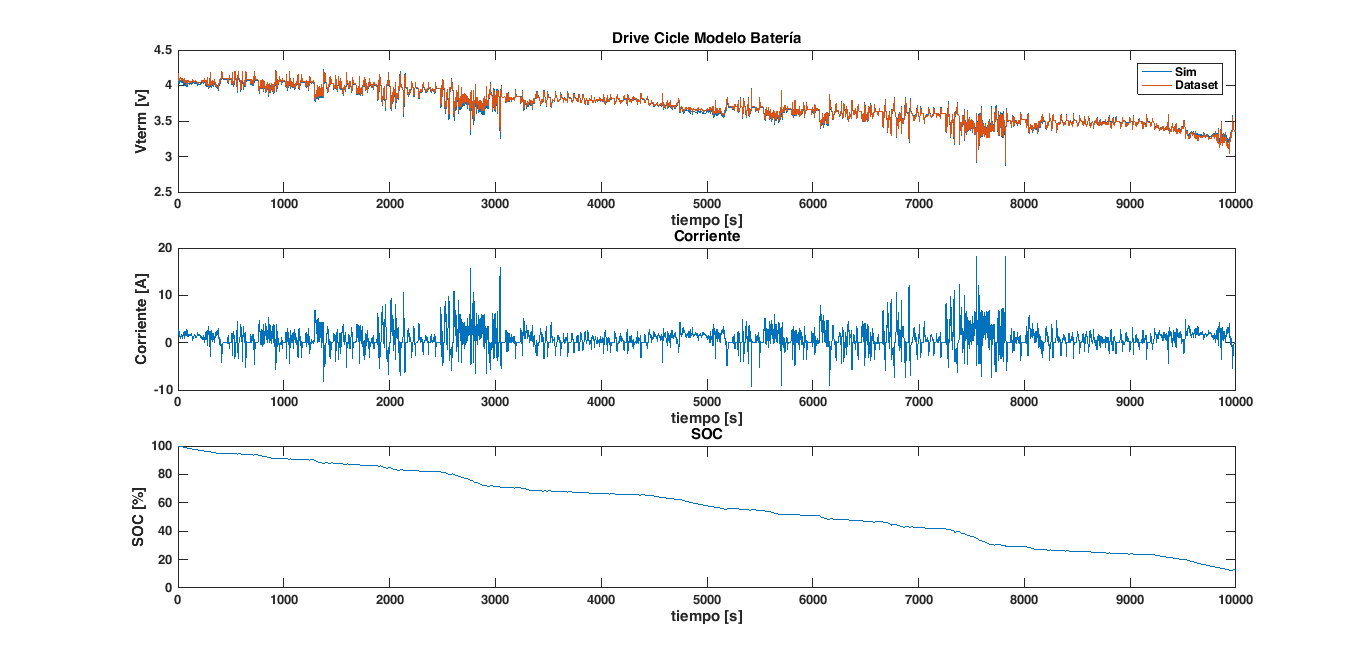
\includegraphics[width=1\linewidth]{Drive_Cicle_Modelo_Bateria.png}
    \caption{Drive Cicle - Modelo Vs Data}                             
    \label{fig:DC_modVsData}                                          
\end{figure}

\subsection{Tiempo de muestreo}

Al trabajar con estrategias de control basadas en microcontroladores y sensores
digitales nos encontramos con la necesidad de discretizar los procesos y tener
en cuenta los tiempos de muestreo.

El teorema de Nyquist-Shannon nos permite calcular un límite inferior a la
frecuencia de muestreo, ya que este establece que si la frecuencia de muestreo
cumple con la condición \ref{nyquist_condition} siendo $f_s$ la frecuencia de
muestreo y $F_{MAX}$ la máxima frecuencia presente en la señal, se podrá
reconstruir la señal sin perder información \cite{Nyquist1928},
\cite{Shannon1949}.  Por el contrario, si la señal y la frecuencia de muestreo
no son las adecuadas se produciría \emph{aliasing}.

\begin{equation}
	f_s > 2 F_{MAX}
	\label{nyquist_condition}
\end{equation}

Dado el sistema de Ecuaciones \ref{SS_model_eq} el cual es una representación de
nuestro sistema en espacio de estados, podemos calcular los valores de los polos
sabiendo los Eigenvalores o Autovalores de la matriz de evolución A.

Además, la matriz de evolución de nuestro sistema es diagonal por lo que los
autovalores y subsecuentemente los polos se corresponden con los elementos
$A_{nn}$ con $n=\{1;2;3\}$.

Tomando el valor del máximo valor absoluto entre los elementos $A_{nn}$ de las
todas matrices A obtenidas para cada valor de $SoC$ obtuvimos de la Ecuación
\ref{eq_polo_rapido}, el valor del polo más rapido:

     \begin{equation}
     	MAX  \left \|A_{nn}(Soc)\right \| = \omega = 6.6379 rad/s
     	\label{eq_polo_rapido}
     \end{equation}

Dado que la frecuencia de corte $f_c$ asociada al polo más rapido se calcula
según la Ecuación \ref{ang_vs_frec} obtenemos $F$ y reemplazamos en
\ref{nyquist_condition} obteniendo nuestra frecuencia mínima de muestreo
$f_{smin}$ de la Ecuación \ref{nyquist_condition_2}.

\begin{equation}
	F = \frac{\omega}{2 \pi} = 1.056 Hz
	\label{ang_vs_frec}
\end{equation}

\begin{equation}
	f_{s min} > 2 F = 2.113 Hz
	\label{nyquist_condition_2}
\end{equation}

En la figura \ref{system_bode} se observa que a partir de $\omega = 10 rad/s$ la
ganancia esta determinada por $-20log(R_{0})\approx-30dB$, lo cual es coherente
con los calculos previos.

\begin{figure}[h!]
	\begin{center}
		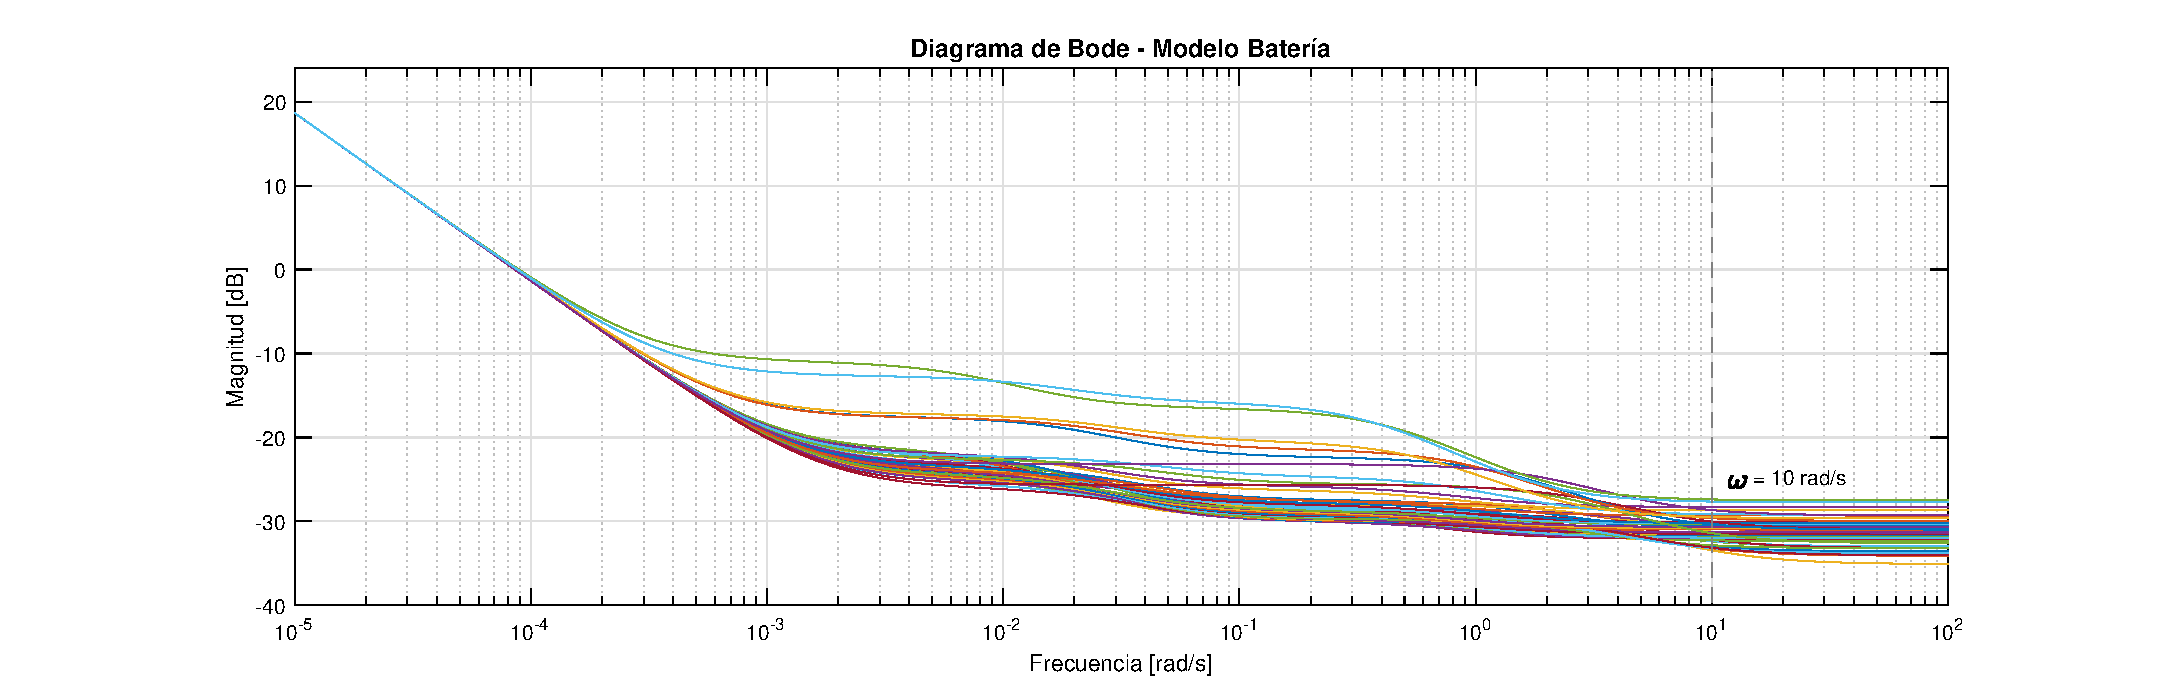
\includegraphics[width=1\textwidth]{bode_amplitud_w_grid.eps}
		\caption{Diagrama de Bode del sistema.}
		\label{system_bode}
	\end{center}
\end{figure}
\FloatBarrier

Los tiempos de procesamiento del Microcontrolador del filtro de Kalman y los
sensores en conjunto son de 10ms por lo que la frecuencia de muestreo de nuestro
sistema es $100 Hz$ cumpliendo con la condición \ref{nyquist_condition}.

\subsection{Desarrollo de la estimaci\'on de \acrshort{SOC}}

Como se detalla en la Secci\'on \ref{algSoc}, el \acrshort{SOC} y su
estimaci\'on son factores claves para el diseño y desarrollo de un
\acrshort{BMS} apropiado para nuestra aplicaci\'on en particular. Como el mismo
solo puede ser estimado, la misma debe ser robusta con respecto a:

\begin{itemize}
    \item Valor de \acrshort{SOC} incorrecto.
    \item Ruido y \emph{offset} en la medici\'on.
    \item Dispersi\'on de par\'ametros entre celdas provenientes del mismo
        fabricante.
\end{itemize}

Tambi\'en se menciona anteriormente la gran variedad de algoritmos disponibles
para realizar la estimaci\'on de esta variable no medible en tiempo real. En el
presente trabajo se desarrollaron dos algoritmos, uno basado en un filtro
observador, como lo es el Filtro de Kalman y otro algoritmo basado en redes
neuronales, cuyo desarrollo se describe a continuaci\'on.

\subsubsection{Algoritmo basado en el Filtro de Kalman}

El algoritmo de estimaci\'on del \acrshort{SOC} se basa en el uso 
de un Filtro de Kalman Extendido en conjunto con el modelo desarrollado en la 
Secci\'on \ref{dev_batt_model}. Como se detalla en la Secci\'on
\ref{KalmanFilterMethod}, en conjunto con el desarrollo matem\'atico del
m\'etodo en el Anexo \ref{matKalman}, el proceso consiste en obtener un modelo
en ecuaciones de estados del sistema en cuesti\'on e identificar la variable a 
observar para poder implementar el algoritmo del filtro.

\subsubsubsection{Modelo de la celda en ecuaciones de estados}

Para la implementaci\'on de este algoritmo es necesario obtener un modelo en
espacio de estados de la celda, como se muestra en el siguiente sistema de
Ecuaciones \emph{(Ecs. \ref{ss_model_generic})}:

\begin{align}
    \dot{x}(t) = Ax+Bu	\nonumber\\
    y(t)=Cx+Du
    \label{ss_model_generic}	
\end{align}

partiendo del modelo desarrollado en la Secci\'on \ref{dev_batt_model}, la
salida del mismo es descripto por la Ecuaci\'on \ref{v_out_randles},

\begin{equation}
    v(t) = v_{OCV}(SOC) - \left[i(t) \times R_0\left(SOC\right)  + v_{C_1}\left(t,
    SOC\right) + v_{C_2}\left(t, SOC\right)\right] \label{v_out_randles}
\end{equation}

\noindent La fuente de tensión controlada $V_{OCV}(SOC)$ es linealizada para 
cumplir con la exigencia del filtro en utilizar un modelo linealizado sobre un
punto de operaci\'on, en este caso, se obtiene una Ecuaci\'on de la forma
\ref{ocv_linearized}, cuyos parametros son optimizados con el uso de la
librer\'ia \emph{polyfit} de \emph{Matlab} y los datos obtenidos en la etapa de
pre-procesamiento descripta en la Secci\'on \ref{data_preprocessing}. En la 
Figura \ref{soc_linealized} se observa el resultado de la linealizaci\'on y
parametrizaci\'on de la curva.

\begin{equation}
    v_{OCV}(SoC) = SoC \times K_e + V_{OCV_0} 
    \label{ocv_linearized}
\end{equation}

\begin{figure}[h!]
    \begin{center}
	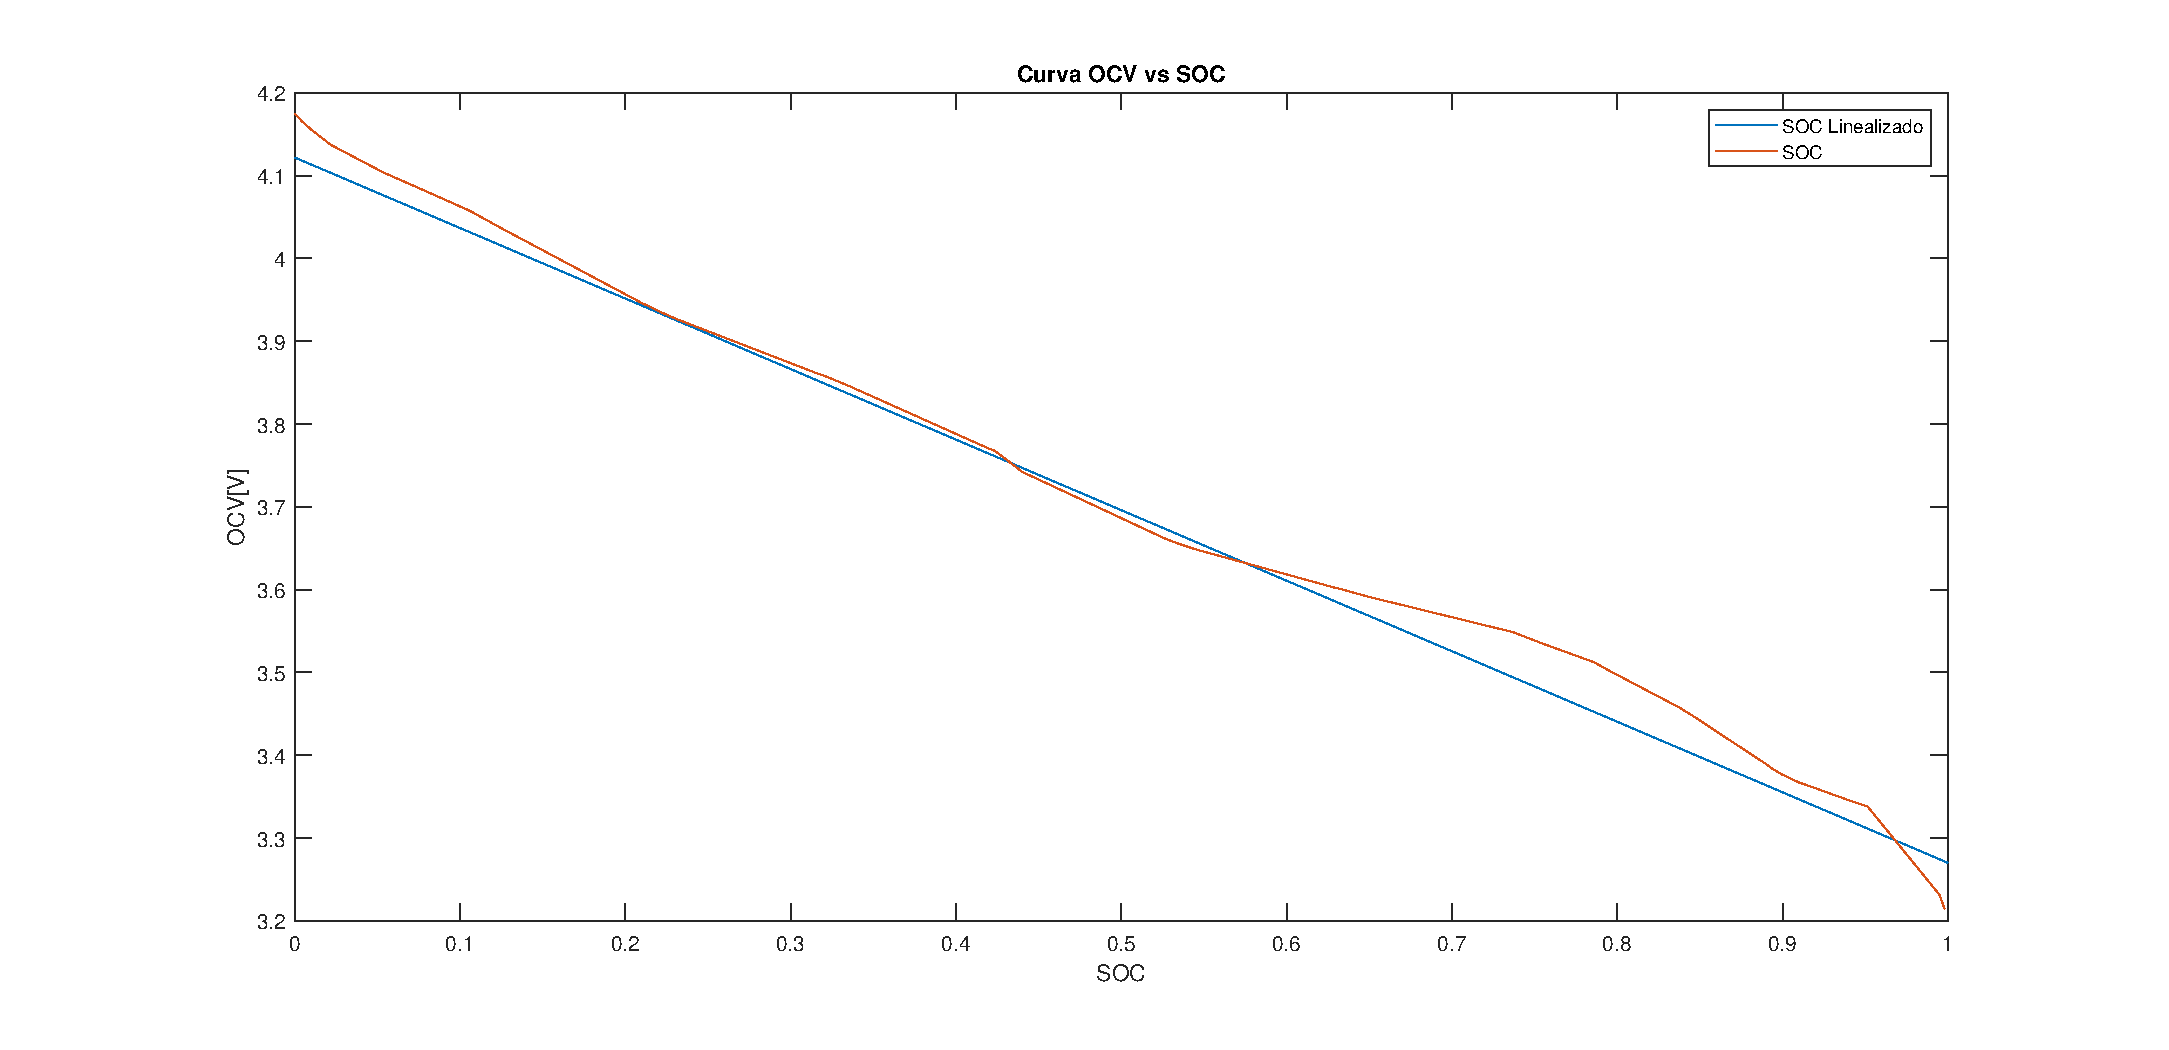
\includegraphics[width=1\textwidth]{SOC_vs_OCV.eps}
    \caption{Curva comparativa de \acrshort{OCV} en base al \acrshort{SOC} 
    entre la versi\'on linealizada (azul) y la no-linealizada (naranja).} 
	\label{soc_linealized}
    \end{center}
\end{figure}
\FloatBarrier

Reemplazando \ref{ocv_linearized} en \ref{v_out_randles}, se obtiene la
Ecuaci\'on \ref{v_out_randles_linearized},

\begin{equation}
    v(t) = SoC \times K_e + V_{OCV_0} - \left[i(t) \times R_0\left(SOC\right) 
        + v_{C_1}\left(t, SOC\right) + v_{C_2}\left(t, SOC\right)\right] 
    \label{v_out_randles_linearized}
\end{equation}

Dado que la Ecuaci\'on \ref{v_out_randles_linearized} representa la salida del 
sistema, esta Ecuaci\'on es el equivalente a la expresi\'on de $y(t)$ en el 
sistema de Ecuaciones de estado \emph{(Ec. \ref{ss_model_generic})}

Por lo tanto, la expresi\'on de $y(t)$ en el sistema de Ecuaciones
\ref{ss_model_generic} es reemplazado por la Ecuaci\'on \ref{v_out_randles}, que
a su vez se desarollada matricialmente, como se puede observar en la
Ecuaci\'on \ref{v_out_randles_mat},

\begin{equation}
    y(t) = v(t) = \begin{bmatrix} -1 -1 -K_e \end{bmatrix} \times 
    \begin{bmatrix} V_{C_1}(t, SoC) \\ V_{C_2}(t, SoC) \\ SoC(t) \end{bmatrix} +
    \begin{bmatrix} R_0(SoC) \end{bmatrix} i(t)\label{v_out_randles_mat}
\end{equation}

a partir de esta expresi\'on se puede deducir que las variables de estado 
($x(t)$) es el voltaje en ambos capacitores ($\mathrm{V_{C_1}}$ y 
$\mathrm{V_{C_2}}$) y el \acrshort{SOC} de la bater\'ia, por otro lado, la 
variable de entrada es la corriente ($i(t)$) y la matriz D es $R_0(SoC)$, 
obteniendo el siguiente sistema de Ecuaciones de estados 
\emph{(Ec. \ref{randles_ss_incomplete})}

\begin{align}
    \begin{bmatrix}
        \dot{V}_{C_1}(t, SoC) \\ \dot{V}_{C_2}(t, SoC) \\ \dot{SoC}(t)
    \end{bmatrix} &= 
    A\times\begin{bmatrix}V_{C_1}(t, SoC) \\ V_{C_2}(t, SoC) \\ SoC(t)\end{bmatrix}
    +
    D\times i(t)\nonumber \\
    v(t) &= \begin{bmatrix} -1 -1 -K_e \end{bmatrix} \times 
    \begin{bmatrix} V_{C_1}(t, SoC) \\ V_{C_2}(t, SoC) \\ SoC(t) \end{bmatrix} +
    \begin{bmatrix} R_0(SoC) \end{bmatrix} i(t)\label{randles_ss_incomplete}
\end{align}

el \acrshort{SOC} es calculado por el m\'etodo de acumulaci\'on de
corriente, cuya expresi\'on se observa en la Ecuaci\'on
\ref{soc_mod_integration},

\begin{equation}
    SoC(t) = SoC_{0}  - \int \frac{i\left(t\right)}{3600 S_{c,a}} dt
    \label{soc_mod_integration}
\end{equation}

donde $\mathrm{S_{c,a}}$ es la capacidad actual de la bater\'ia medido en
Ampere-hora [Ah]. Derivando miembro a miembro, se obtiene la Ecuaci\'on
\ref{soc_mod_integration_der},

\begin{equation}
    \dot{SoC}(t) = - \frac{i(t)}{3600S_{c,a}}\label{soc_mod_integration_der}
\end{equation}

Por otro lado, para determinar las expresiones de $V_{C_1}(t)$ y $V_{C_2}(t)$,
se analiza el circuito RC paralelo \emph{(Fig. \ref{tanque_rc})},

\begin{figure}[h!]
    \begin{center}
        \begin{circuitikz}[american]
            \draw (1, 0) to[short,i=$i$] (2, 0);
            \draw (2,0) -- (2,-1) -- (3, -1) to[R=$R_1$] (5,-1) 
            to[short,i=$i_1$] (6, -1) -- (6,0);
            \draw (2,0) -- (2, 1) -- (3, 1) to[C=$C_1$,v=$V_{C1}$] 
            (5, 1) to[short,i=$i_2$] (6, 1) -- (6,0) -- (7, 0);
        \end{circuitikz}
        \caption{Circuito RC paralelo}
        \label{tanque_rc}
    \end{center}
\end{figure}

partiendo de la Ecuaci\'on de carga de un capacitor, la ley de Kirchhoff de
corrientes y la ley de Ohm se obtiene el siguiente sistema de Ecuaciones
\emph{(Ecs. \ref{cap_sist_eq})},

\begin{align}
    i_2(t) &= C_1 \dot{v}_{C_1}(t)\nonumber\\
    i(t) &= i_1(t) + i_2(t)\label{cap_sist_eq}\\
    v_{c_1}(t) &= R_1i_1(t)\nonumber
\end{align}

Despejando $i_1(t)$ en la segunda Ecuaci\'on de \ref{cap_sist_eq}, reemplazando
en la tercera ecuaci\'on y reemplazando $i_2(t)$ por la primer expresi\'on,
obtenemos la Ecuaci\'on \ref{v_cap_reemplazada},

\begin{equation}
    v_{C_1}(t) = R_1i(t) - R_1C_1\dot{v}_{C_1}(t) \rightarrow 
    \dot{v}_{C_1}(t) = \frac{i(t)}{C_1} -
    \frac{v_{C_1}(t)}{R_1C_1}\label{v_cap_reemplazada}
\end{equation}

Por \'ultimo, reemplazando \ref{soc_mod_integration_der} y
\ref{v_cap_reemplazada} en el sistema de ecuaciones de estado, en forma
matricial, finalmente se obtiene el sistema de Ecuaciones 
\ref{ss_randles_complete} correspondiente al circuito de Randles de segundo
orden,

\begin{align}
    \begin{bmatrix}
        \dot{V}_{C_1}(t, SoC) \\ \dot{V}_{C_2}(t, SoC) \\ \dot{SoC}(t)
    \end{bmatrix} &= 
    \begin{bmatrix}
        -\frac{1}{R_1C_1} & 0 & 0\\
        0 & -\frac{1}{R_2C_2} & 0\\
        0 & 0 & 0
    \end{bmatrix}
    \times\begin{bmatrix}V_{C_1}(t, SoC) \\ V_{C_2}(t, SoC) \\ SoC(t)\end{bmatrix}
    +
    \begin{bmatrix}
        \frac{1}{C_1} \\ \frac{1}{C_2} \\ \frac{1}{3600S_{c,a}}
    \end{bmatrix}
    \times i(t)\nonumber \\
    v(t) &= \begin{bmatrix} -1 & -1 & -K_e \end{bmatrix} \times 
    \begin{bmatrix} V_{C_1}(t, SoC) \\ V_{C_2}(t, SoC) \\ SoC(t) \end{bmatrix} +
    \begin{bmatrix} R_0(SoC) \end{bmatrix} i(t)\label{ss_randles_complete}
\end{align}

\newpage

\subsubsubsection{Criterio de observabilidad}

Linealizado el sistema y obtenido el sistema de ecuaciones del modelo,
el\'ectrico de Randles, solo resta determinar si el sistema es observable. Un
sistema de ecuaciones de estados es observable, si y solo si, su matriz de
observabilidad, valga la redundancia, es observable, es decir si su determinante 
es diferente a cero y la matriz de observabilidad tiene un rango n 
(orden del sistema). La matriz de observabilidad est\'a dada por la Ecuaci\'on 
\ref{observation_matrix},

\begin{equation}
    O = \begin{bmatrix}
        C\\
        CA\\
        CA^2\\
        \vdots\\
        CA^{n-1}
        \end{bmatrix}\label{observation_matrix}
\end{equation}

En este caso, n es igual a tres, dado que el modelo de Randles es un sistema de 
segundo \'orden, por lo tanto, la matriz O est\'a dada por la Ecuaci\'on 
\ref{obs_matrix_randles},

\begin{equation}
    O = \begin{bmatrix}
        -1 & -1 & -K_e \\
        \frac{1}{R_1C_1} & \frac{1}{R_2C_2} & 0 \\
        \frac{1}{\left(R_1C_1\right)^2} & \frac{1}{\left(R_2C_2\right)^2} & 0
        \end{bmatrix}\label{obs_matrix_randles}
\end{equation}

aplicando el determinante de una matriz sobre la Ecuaci\'on
\ref{obs_matrix_randles} obtenemos la expresi\'on \ref{det_obs_matrix_randles}

\begin{align}
    det\left(O\right) &= 0 + 0 -K_e \frac{1}{R_1C_1\left(R_2C_2\right)^2} + 
                        K_e \frac{1}{R_2C_2\left(R_1C_1\right)^2} - 0 -
                        0\nonumber\\
                      &= K_e \left(\frac{1}{R_2C_2\left(R_1C_1\right)^2} - 
                                   \frac{1}{R_1C_1\left(R_2C_2\right)^2}\right)
                                   \label{det_obs_matrix_randles}
\end{align}

Por lo tanto la matriz O es observable, si y solo si, se cumple que los
par\'ametros de los circuitos RC del modelo de Randles no sean iguales, ya que
en caso contrario la determinante ser\'ia igual a cero. Por otro lado, se observa
claramente que la matriz O es de dimensi\'on 3x3, por lo tanto es una matriz de
orden 3, concluyendo finalmente que el sistema de Randles es observable, por 
ende, se puede implementar el Filtro de Kalman para determinar el \acrshort{SOC} 
de la celda.

Finalmente, considerando un sistema de ecuaciones de la siguiente forma \emph{(Ecs.
\ref{ss_with_noise})},

\begin{align}
    \dot{x} = Ax + Bu + \eta_x\nonumber\\
    y = Cx + Du + \eta_y\label{ss_with_noise}
\end{align}

donde $\eta_x$ y $\eta_y$ es ruido Gaussiano que afecta el estado y la salida
del sistema, si se cumple que:

\begin{itemize}
    \item El sistema de Ecuaciones \ref{ss_with_noise} es estoc\'astico.
    \item $\eta_x$ y $\eta_y$ son variables representadas por ruido gaussiano
        con media cero y varianzas $Var\left(\eta_x(t)\right) = Q$,
        $Var\left(\eta_y(t)\right) = R$ y la covarianza entre ambas variables
        est\'a dada por $Cov\left(\eta_x(t), \eta_y(y)(t)\right) = N$.
    \item el estado inicial es un vector gaussiano con covarianza
        $Cov\left(x(0)\right) = P_0$ y media $E\left(x(0)\right) = x_0$
\end{itemize}

es posible considerar el observador de la Ecuaci\'on \ref{ss_kalman_gain},

\begin{align}
    \dot{\hat{x}} &= A\hat{x} + Bu + K(t)(y - \hat{y})\nonumber\\
    \hat{y} &= C\hat{x} + Du \label{ss_kalman_gain}
\end{align}

donde $K(t)$ es la ganancia de Kalman, cuyo objetivo, como se menciona en la
secci\'on \ref{KalmanFilterMethod}, es minimizar la covarianza del error de
estimaci\'on. 

\newpage

Para poder implementar el Sistema de Ecuaciones en \ref{ss_kalman_gain} sobre
el modelo de Randles es necesario proveer las matrices que proporcionan valores 
de varianza sobre las incertezas del modelo (Q) como tambi\'ien los valores de
varianza sobre el ruido al que est\'an sometidas las variables de medici\'on
(R), por el otro lado, tambi\'en es necesario proveer el estado inicial del
sistema ($x_0$) como tambi\'en su covarianza inicial ($P_0$).

En primer instancia, se propone que el estado inicial de la bater\'ia es
conocido, es decir, cuando el \acrshort{BMS} comienza a operar, se asume que la
bater\'ia se encuentra en un estado de reposo lo suficientemente largo como para
poder relacionar de forma directa el \acrshort{OCV} con el \acrshort{SOC}, por
lo tanto, los valores de la matriz $\mathrm{P_0}$ son acotados en valores muy
bajos. Esto se puede observar en la Ecuaci\'on \ref{p_inicial}.


\begin{equation}
    \begin{array}{llll}
	P_0 & = & \begin{bmatrix}
        1\times10^{-7}  & 0              & 0 \\
        0               & 1\times10^{-7} & 0 \\
        0               & 0              & 1\times10^{-7} \\
	\end{bmatrix} 
    \end{array}
    \label{p_inicial}
\end{equation}

Teniendo en cuenta lo mencionado, el estado inicial del sistema est\'a dado por
la Ecuaci\'on \ref{x_inicial_sistema}, donde se puede observar que no hay
corriente circulante y que la 3er fila, que corresponde con el \acrshort{SOC} de
la celda, est\'a relacionado directamente con el \acrshort{OCV},

\begin{equation}
    \begin{array}{llll}
	x_0 & = & \begin{bmatrix}
	    0 \\
	    0 \\
        OCV(SOC) \\
	\end{bmatrix} 
    \end{array} \label{x_inicial_sistema}
\end{equation}

Para acotar un valor de la matriz R, se toma en cuenta la exactitud del sensor
de tensi\'on que se implementa para este proyecto, en este caso, el proyecto
utiliza como \emph{Frontend Anal\'ogico} el \acrshort{IC} BQ76PL536A, cuyo
fabricante especifica una exactitud de $\mathrm{\pm 1mV}$, por lo tanto, R da un 
valor equivalente al expresado en la Ecuaci\'on \ref{valor_r} medido en mV

\begin{equation}
    R = 1  \label{valor_r}
\end{equation}

Finalmente, la matriz Q expresa la incerteza del modelo desarrollado en la 
Secci\'on \ref{dev_batt_model}. Para obtener los valores de esta matriz se
analizaron los resultados obtenidos en los resultados del modelo en la Secci\'on 
\ref{val_param_modelo}, observando las variaciones de las tensiones de cada
capacitor en conjunto con los valores de OCV(SOC), se acotaron y
ajustaron los valores de la matriz Q a los que se observan en la Ecuaci\'on
\ref{valor_q},

\begin{equation}
    \begin{array}{llll}
	Q & = & \begin{bmatrix}
	    4.5\times10^{-3} & 0 & 0 \\
	    0 & 5\times10^{-4} & 0 \\
	    0 & 0 & 1\times10^{-10} \\
	\end{bmatrix} 
    \end{array} \nonumber
\end{equation}

Finalmente, se desarroll\'o el algoritmo de Kalman en un script de \emph{Matlab}
y se ensay\'o el algoritmo en conjunto con el modelo bajo el mismo set de datos
utilizado en \ref{ensayo_HPPC}. Como resultado se obtuvo las gr\'aficas que se
observan en la Figura \ref{kalman_result_matlab}, en la que se puede deducir que
se obtiene un error m\'aximo de 3\%, aceptable para los objetivos del trabajo.

\begin{figure}[h!]
    \begin{center}
        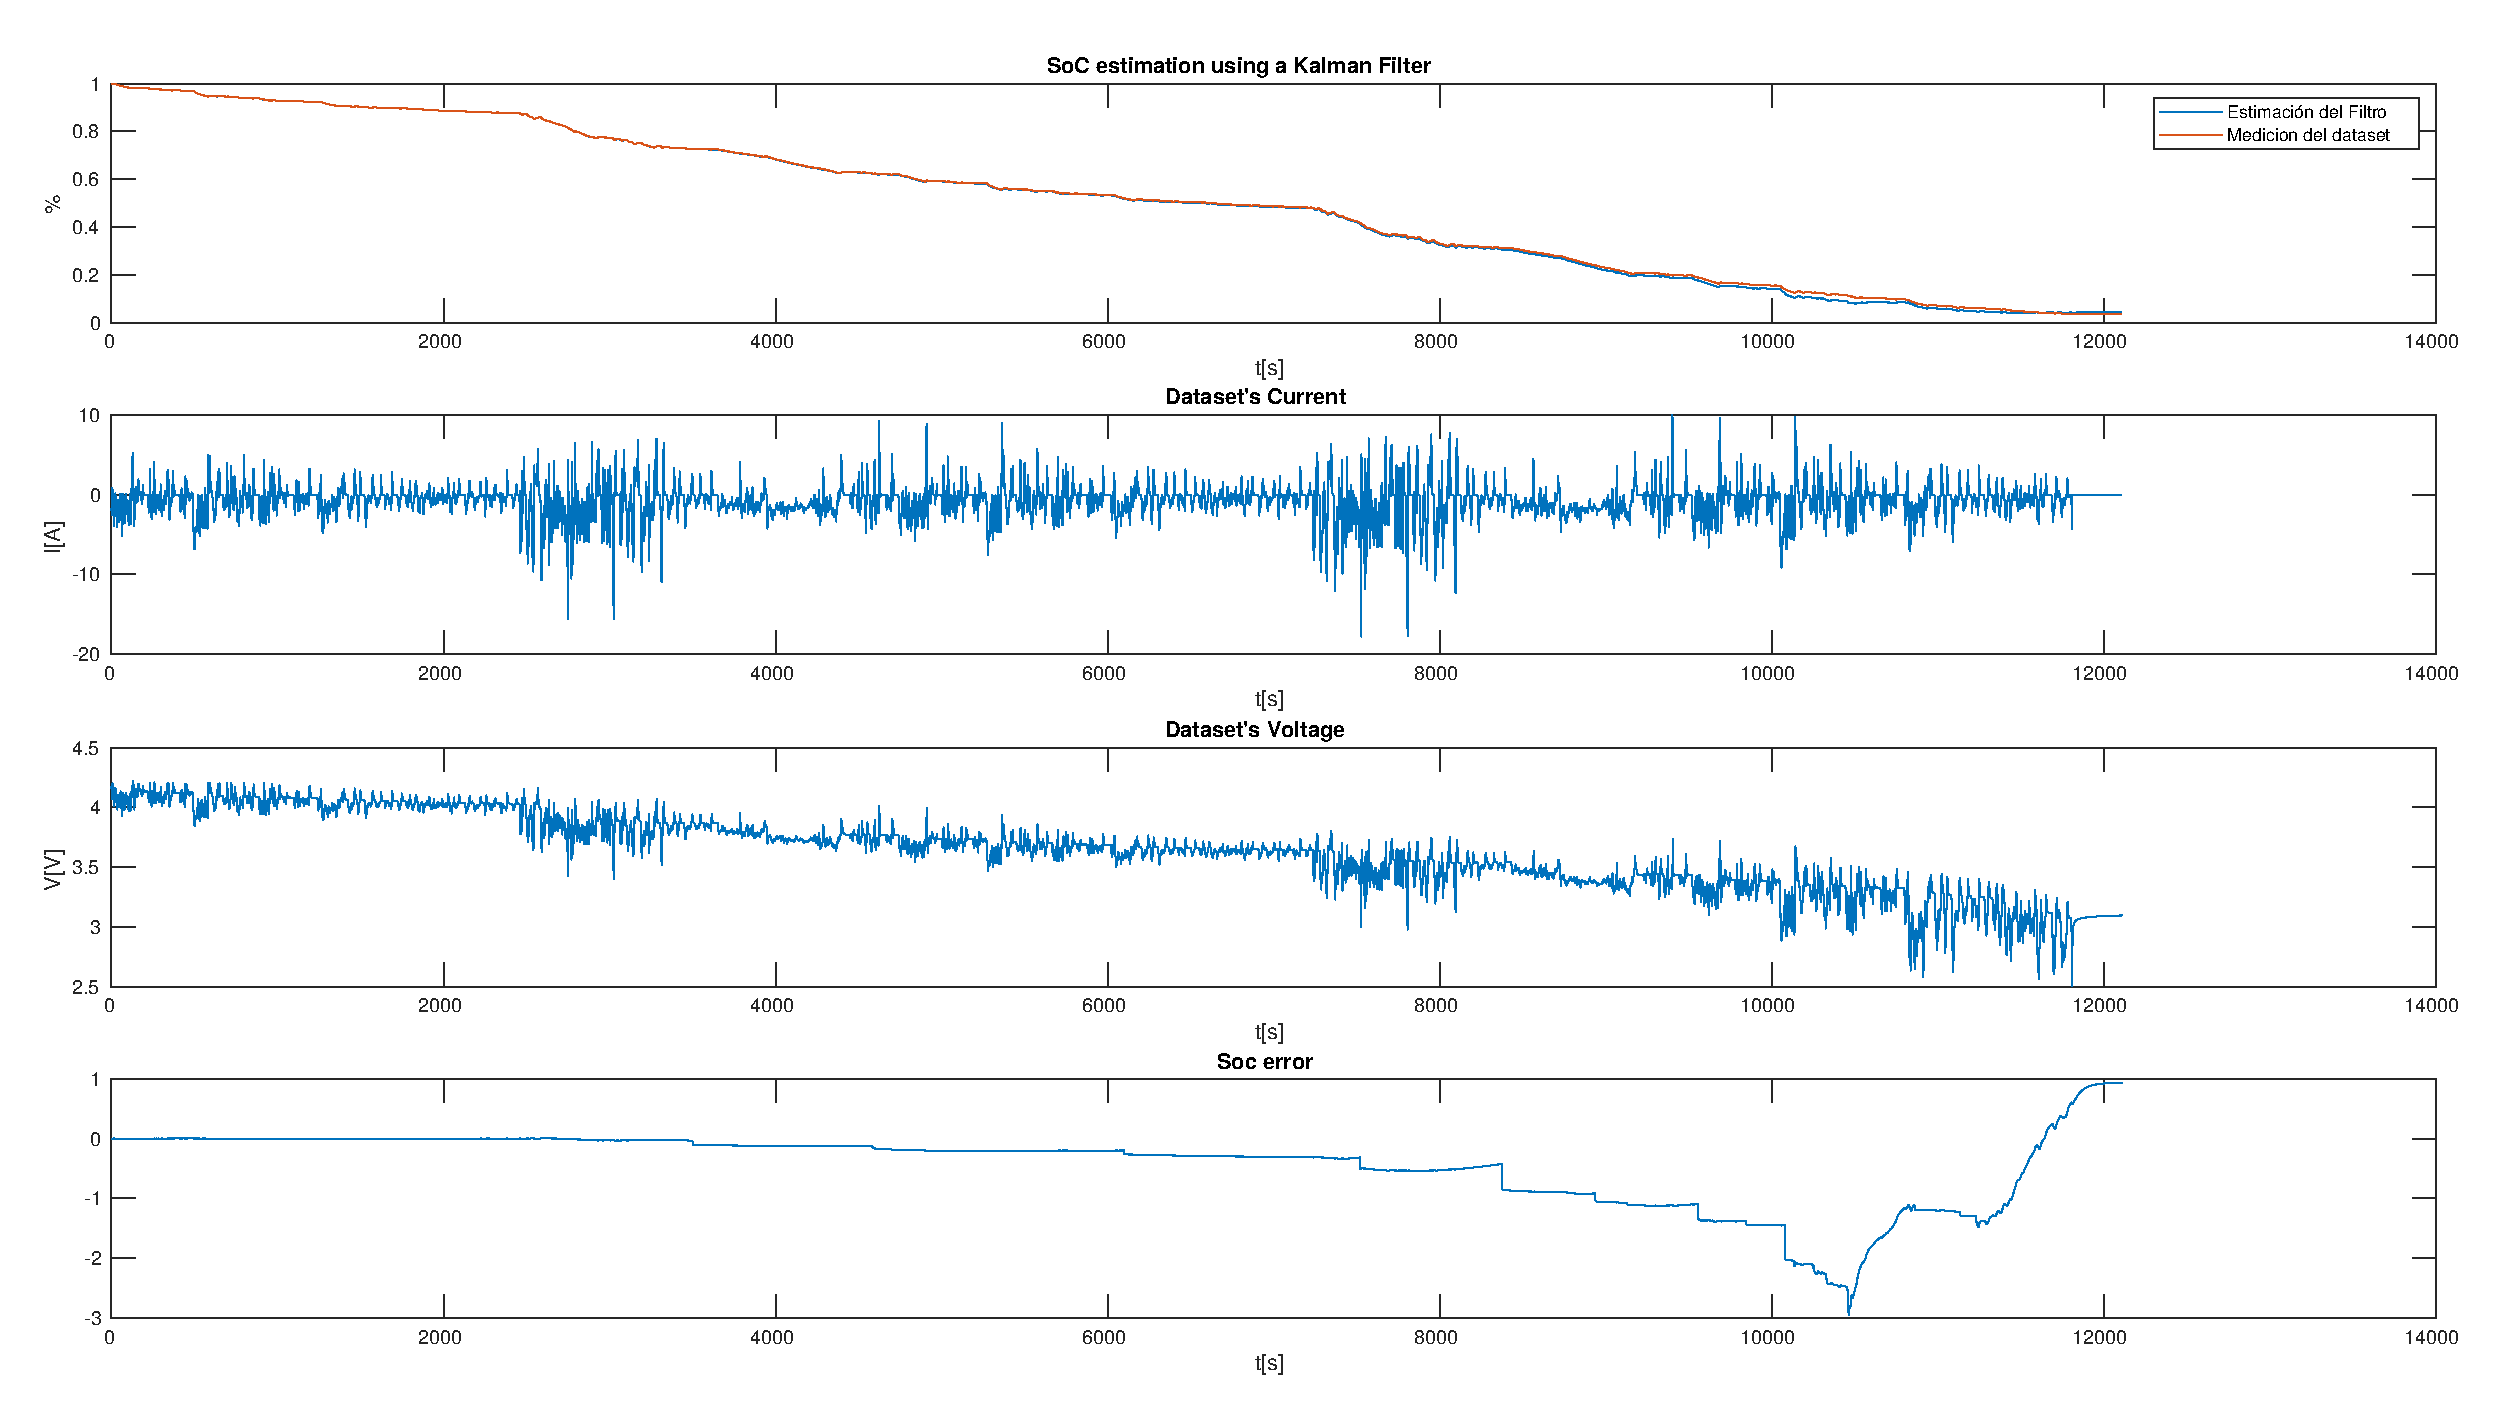
\includegraphics[width=1\textwidth]{kalman_result_matlab.eps}
        \caption{1ra Gr\'afica: Estimaci\'on del \acrshort{SOC} vs
        \acrshort{SOC} del ensayo. 2da Gr\'afica: Corriente del dataset. 3ra
        Gr\'afica: Voltaje del dataset. 4ta Gr\'afica: Error en la estimaci\'on
        del \acrshort{SOC}} 
        \label{kalman_result_matlab}
    \end{center}
\end{figure}

\newpage

\subsection{Unidad de procesamiento}

\subsubsection{Tecnología seleccionada - STM32F407VG}

Actualmente existen en el mercado un sin número de microcontroladores de
distintos proveedores que implementan diferentes arquitecturas. La naturaleza de
los desafios matemáticos que plantea el desarrollo del \acrshort{BMS} y el
rendimiento computacional requerido para el procesamiento en tiempo real fueron
dos de los pilares fundamentales para la selección e implementación del
Microcontrolador \textbf{STM32F407VG} de la empresa \emph{STMicroelectronics}. 

El \textbf{STM32F407VG} es un microcontrolador de la familia STM32F407xx de la
firma \emph{STMicroelectronics} que implementan un nucleo de alto rendimiento de
32-bits Arm® Cortex®-M4 con arquitectura \acrshort{RISC} y que puede operar a
una frecuencia de hasta 168 MHz.  El nucleo Cortex-M4 implementa dos módulos
fundamentáles para la optimización del proceso de cálculo matemático del
\acrshort{BMS} y el procesamiento en tiempo real. Una unidad de punto flotante
(por sus siglas en ingles \acrfull{FPU}) de precision simple que soporta todas
las instrucciones y tipos de datos Single-Precision data-Processing del nucleo
y un set completo de instrucciones de \acrshort{DSP}. La familia STM32F407xx a
su vez incorpora una memoria FLASH embebida de alta velocidad de hasta 1 Mbyte y
192+4 Kbytes de RAM (\acrfull{SRAM}).

\begin{wrapfigure}{R}{5.5cm}
    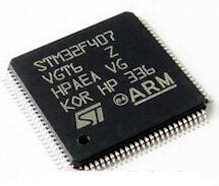
\includegraphics[width=5.5cm]{STM32F407VG.png}
    \caption{STM32f407VG}
    \label{fig:stm32f407vg}                                                            
\end{wrapfigure}                                                                 

Otras características tenidas en cuenta y de las que dispone el \acrshort{CI}
son sus tres módulos ADCs de 12-bits, dos DACs, un \acrshort{RTC} de
bajo consumo, 4 timers de propósitos generales y una serie de módulos de
interface de comunicaciones entre los que destacan el módulo \acrshort{CAN} y la
interfaz de puerto Serie utilizadas en el proyecto \acrshort{BMS}.

El empaquetado del \acrshort{CI} seleccionado es \acrfull{LQFP} de 100 pines.

\begin{itemize}                                                                  
    \item Nucleo: 

        \begin{itemize}                                                                  
            \item  32-bits Arm Cortex-M4 @ 168 MHz     
            \item  210 \acrshort{DMIPS} - $1.25$\acrshort{DMIPS}/MHz
            \item \acrfull{NVIC}
            \item Debug: \acrfull{SWD} + JTAG interfaces
            \item [+] Unidad de Punto Flotante \acrshort{FPU} 
            \item [+] Acelerador Adaptativo de Tiempo Real \acrshort{ART} 
            \item Modos de funcionamiento Run, Idle and Sleep                          
        \end{itemize}

    \item Clock:

        \begin{itemize}
            \item Cristal externo 4-to-26 MHz 
            \item Oscilador interno 16 MHz (res: 1\%)
            \item Oscilador interno RTC 32 KHz 
        \end{itemize}

    \item Memoria                                       

        \begin{itemize}                                                                  
            \item Flash 1 Mbyte 
            \item \acrshort{SRAM} $192+4$ Kbytes  
            \item \acrshort{OTP} 512 bytes 
        \end{itemize}

    \item Conectividad

        \begin{itemize}                                                                  
            \item 2x SPI, 3x $I^2C$, 2x $I^2S$
            \item Ethernet MAC 10/100 (IEEE 1588)
            \item 6x UART 
            \item 2x CAN 2.0B 
            \item SDIO 
            \item USB 2.0 
        \end{itemize}

    \item IOs
    \item PWM 2x 16-bits
    \item ADC 3x 12-bit, 24 canales, hasta 500k muestras por segundo              
    \item DAC 2x 12-bit 
    \item DMA 16-streams
    \item Timer 12x 16-bis + 2x 32-bits 
    \item LCD paralelo, 8080/6080 
    \item CRC
    \item RTC
\end{itemize}                                                                    
                                                                                 
Se adjunta en \autoref{seq:appendix} el esquemático correspondiente del circuito 
desarrollado bajo el nombre $TODO.pdf$.                   
                                                                                 
\subsubsection{Alimentación}

Para alimentar la unidad de procesamiento del \acrshort{BMS} se desarrolla e
implementa un convertidor de tensión DC-DC basado en el circuito integrado
TPS54331 de tecnología switching tipo Step Down de la firma \emph{Texas
Instruments}. En la Figura \ref{fig:TPS54332D_common_implementation} se puede
observar su implementación modelo. 

\begin{figure}[h!]
    \begin{center}
	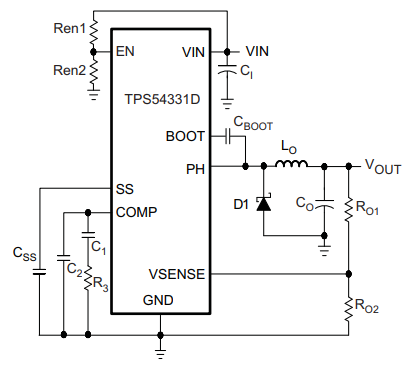
\includegraphics[width=0.4\linewidth]{assets/TPS54332D_common_implementation.png}
	\caption{Implementación Tipo - TPS54332D}
	\label{fig:TPS54332D_common_implementation}
    \end{center}	
\end{figure}

El criterio de selección se basó en la necesidad de optimizar el consumo de
energía del pack de batería, priorizando el máximo ahorro. Por lo que la
tecnología switchin se preseta como una solución superadora frente a otras
opciones, como ser los reguladores transistorizados, de menor eficiencia
energética.

El TPS54331 implementa un convertidor de energía tipo buck de hasta 28 V y 3 A
que integra en la propia pastilla de silicio un MOSFET de bajo RDS(on) a la
salida simplificando el circuito y abaratando costos.
Para incrementar su performance durante los transitorios de linea y carga y para
disminuir la disipación de energía el dispositivo implementa un control por
corriente a frencuencia constante el cual permite reducir la capacidad de salida
y simplificar el diseño del filtro de salida y su compensación. El \acrshort{CI}
opera a una freciencia pre fijada de $f_{sw}=570 KHz$.
El empaquetado del \acrshort{CI} implementado es del tipo SOIC de 8-pines. El
mismo no requiere disipación energética externa adicional y la misma se realiza
a través del plano de masa del \acrshort{PCB}.

\begin{figure}[h!]
    \centering
    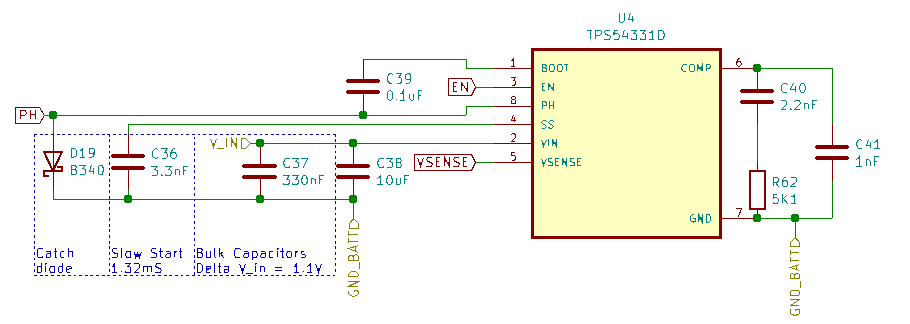
\includegraphics[width=0.8\linewidth]{hardware/3v3/3v3_IC.png}
        \caption{Implementación TPS54331 Texas Instruments}
        \label{fig:3v3_IC}
\end{figure}
\FloatBarrier

El set-point del voltaje de salida se configura externamente seteando un voltaje
en el pin SENSE del \acrshort{CI} a partir del divisor resistivo presentado en
la figura \ref{fig:3v3_set_point}. La relación del voltaje de salida y la
tensión sensada se presenta en la Ecuación \ref{eq:3v3_vout}.

El voltaje aplicado en SENSE es comparado al interior del \acrshort{CI} contra
una referencia $V_{ref} = 0.8 V \pm2\%$ la cual define si el voltaje de
salida se haya por debajo o por encima del valor deseado. 

La Ecuación \ref{eq:3v3_vout} que define el voltaje de salida $V_{out}$ a partir
de hacer $ V_{SENSE} \equiv V_{ref}$ será entonces:

\begin{equation}
    V_{out} = V_{ref}*(\frac{R_{5}}{R_{6}}-1) = 3.3 V
    \label{eq:3v3_vout}
\end{equation}

\begin{figure}[h!]
    \centering
    \begin{subfigure}[t]{0.45\textwidth}
        \centering
        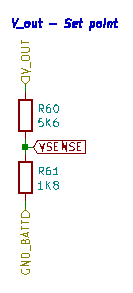
\includegraphics[width=0.35\linewidth]{hardware/3v3/3v3_set_point.png}
        \caption{Circuito de fijación de Set-Point de tensión de salida
        $V_{out}$}
        \label{fig:3v3_set_point}
    \end{subfigure}
    \hfill
    \begin{subfigure}[t]{0.45\textwidth}
        \centering 
        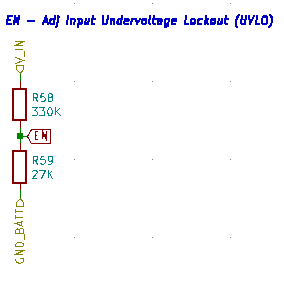
\includegraphics[width=0.75\textwidth]{hardware/3v3/3v3_input_under_voltage.png}
        \caption{Circuito de fijación de Set-Point de tensión de entrada de
        bloqueo }
        \label{fig:3v3_input_under_voltage}
    \end{subfigure}
        \caption{Fijación Set-Points fuente de alimentación 3v3}
        \label{fig:cb_set_point}
\end{figure}
\FloatBarrier

El \acrshort{CI} requiere de una alimentación mayor a $3.5 V$ para operar
correctamente. El pin de Habilitación EN implementa una fuente de corriente
interna que permite ajustar un voltaje mínimo de bloquéo por falta de
alimentación externa a partir de un arreglo de resistencias como se observa en
la Figura \ref{fig:3v3_input_under_voltage}.
Se fijan los voltajes de apagado por falta de alimentación y de encendido
teniendo en cuenta evitar que se consuma energía del pack de batería cuando las
celdas presenten voltajes por debajo de su valor de operación segura.

\begin{align}
    V_{start} &= 16.29V \\
    V_{stop} &= 15.3V \\
    R_{1} &= \frac{V_{star} - V_{end}}{I_{hist}} = 330K\ohm \\
    R_{2} &= \frac{V_{en}}{I_{hist} + 1\mu A} = 27K\ohm 
\end{align}

La figura \ref{fig:3v3_output_filter} corresponde a la etapa de potencia de la
fuente de alimentación tipo buck implementada. La integran un Mosfet canal-N y
un diodo de bootstrap integrado al miso \acrshort{CI}, una inductancia y 1
capacitor, L2 y C42 respectivamente, que funcionan como filtros de ripple a la
salida. También forman parte fundamental de la etapa el capacitor C39 que
funciona como bootstrap del voltaje necesario para excitar el gate del mosfet de
la parte alta. Puede observarse en la imagen \ref{fig:3v3_IC}.

\begin{figure}[h!]
    \centering
    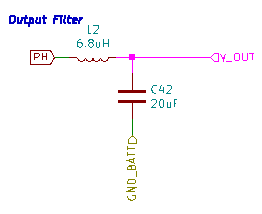
\includegraphics[width=0.3\linewidth]{hardware/3v3/3v3_output_filter.png}
    \caption{Filtro de salida}
    \label{fig:3v3_output_filter}
\end{figure}

La selección de los componente que integran la etapa de salida fue realizada
siguiendo los lineamientos y recomendaciones de la hoja de datos del
\acrshort{CI}. 

Calculamos el valor mínimo de la inductancia sustituyendo los valores de las
condiciones de operación en la ecuación \ref{eq:3v3_L}. Donde $K_{IND}$ es el
coeficiente que representa la cantidad de ripple de corriente en relación a la
corriente de salida.

\begin{equation}
    L_{min} = \frac{V_{out} * (V_{in (max)} - V_{out})}{V_{in (max)}*K_{IND}*I_{out}*f_{sw}} = 6.8\mu H
    \label{eq:3v3_L} 
\end{equation}

Para el cálculo de la capacidad de salida C, se tuvo en cuenta los facores de
diseño como la corriente de ripple, la resistencia serie equivalente
(\acrshort{ESR}) y el voltaje DC que deberá soportar el integrado. El valor de
\acrshort{ESR} es fundamental ya que junto con la capacidad determinan el ripple
del voltaje de salida. El valor seleccionado $ESR_{max} = 47.87 m\ohm$

Calculamos el valor mínimo de la capacidad de salida $C_{0 (min)}$ sustituyendo
los valores de las condiciones de operación en la ecuación \ref{eq:3v3_C}. Donde
$R_{O} = \frac{V_{out}}{I_{out}}$ equivale la impedancia de salida y $F_{CO
(max)}$ a la frecuencia de corte seleccionada, que como regla general se toma
$\frac{f_{sw}}{5} = 25 kHz$ 

\begin{equation}
    C_{o (min)} = \frac{1}{2\pi * R_{0} * F_{CO (max)}} = 6.875\mu F\\
    \label{eq:3v3_C}
\end{equation}

La capacidad de salida seleccionada finalmente fue de $20\mu F$, acorde a los
ensayos experimentales realizados durante el proceso de montaje de la placa. 

\subsubsection{Placa de desarrollo - Discovery}

Para poder realizar en paralelo el desarrollo e implementación del hardware y
del software del \acrshort{BMS}, gran parte del proceso de desarrollo del
software se llevó a cabo sobre el kit de desarrollo Discovery STM32F4DISCOVERY
que implementa el microcontrolador seleccionado STM32F407.

\begin{figure}[h!]
    \centering
    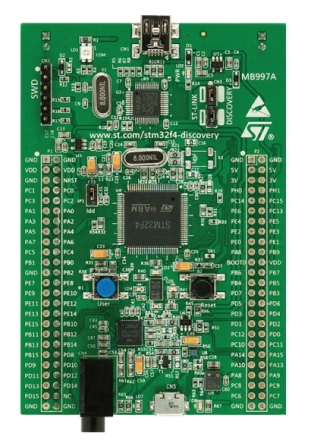
\includegraphics[width=0.3\linewidth, angle=90]{STM32F407VG-discovery.png}
    \caption{Placa de desarrollo Discovery - STM32F4DISCOVERY}
    \label{fig:stm32f4discovery}
\end{figure}

\subsection{Sensor de tensi\'on - Balanceador}

Dada las caracter\'isticas del pack descriptas en la Secci\'on \ref{battery_pack} 
y la diversidad de t\'ecnicas disponibles para el balanceo, con el objetivo de
mantener un diseño simplificado agregando la funcionalidad de ecualizaci\'on al
producto final, se opt\'o por un balanceador basado en una topolog\'ia pasiva 
utilizando resistencias shunt en conjunto con una estrategia de control
cl\'asica que depende del promedio del \acrshort{SOC} entre las 6 celdas,
estableciendo un umbral m\'aximo de variaci\'on entre celdas. 

\newpage

\subsubsection{Tecnolog\'ia Seleccionada - TI bq76pl536a}

Para el desarrollo de esta funcionalidad se opt\'o por el integrado
\emph{BQ76PL536} de la marca \emph{Texas Instruments}. La decisi\'on de utilizar
este integrado con respecto a otras marcas se basa en la Tabla 
\ref{tabla_comparativa_ics}. En la misma se puede observar que el integrado
elegido posee beneficios tanto en funcionalidad, escalabilidad como tambi\'en un
bajo costo con respecto a otros competidores, como por ejemplo, puede extenderse
hasta un pack de 192 celdas conectadas en series, con un valor menor a 9
d\'olares, cuando el resto de los integrados sobre pasan el costo y manejan una
menor cantidad de celdas en serie.

\begin{table}[h!]
    \begin{center}
        \begin{tabular}{llllll}
        \hline
        Modelo     & Fabricante        & Protocolo de CX    & Cant. de celdas & Escalable?          & Costo (u\$s) \\ \hline
        LTC6804    & Analog Devices    & SPI                & 12              & Hasta 100 celdas    & 21.28        \\
        BQ76PL536A & Texas Instruments & SPI                & 6               & Hasta 192 celdas    & 8.83         \\
        MC33772B   & NXP               & SPI                & 3               & No especifica       & 20.74        \\
        MAX14920/1 & Maxim             & SPI                & 16              & No                  & 9.84         \\
        L9963      & STM Electronics   & SPI                & 14              & No                  & 18.36        \\        
        \hline
        \end{tabular}
    \end{center}
    \caption{Comparaci\'on de \acrshort{IC}s dedicados al balanceo pasivo de
    celdas de litio-ion.}
    \label{tabla_comparativa_ics}
\end{table}

\begin{minipage}{0.5\textwidth}
El dispositivo es un monitor y protector de bater\'ias compuestos por 3 a 6
celdas conectadas en serie, que pueden acoplarse entre si para extenderse a 192
celdas. El mismo integra un frontend anal\'ogico (\acrshort{AFE}, del ingl\'es
\acrlong{AFE}) en conjunto con un conversor anal\'ogico-digital (\acrshort{ADC},
del ingl\'es \acrlong{ADC}), utilizado para medir de forma precisa el voltaje de
cada celda. Por el otro lado, tambi\'en posee dos \acrshort{ADC}s para leer la
temperatura del pack de bater\'ias.\\
\\
Adem\'as de la temperatura, tambi\'en  se monitorea el sobrevoltaje y el bajo
voltaje por canal, es decir, por cada celda para tomar las medidas de
protecci\'on necesarias, estas tres variables de protecci\'on pueden ser
configuradas por el usuario a trav\'es del puerto SPI que provee el dispositivo
para escribir los registros internos.\\
\\
Finalmente, el mismo puede soportar bater\'ias de hasta 192 celdas acoplando
varios integrados entre si, a trav\'es de un bus SPI en cadena. Un esquem\'atico
simplificado de \'este tipo de topolog\'ia del dispositivo se puede observar en
la Figura \ref{bq76_simplified_schematic}
\end{minipage}
\begin{minipage}{0.5\textwidth}
    \begin{center}
        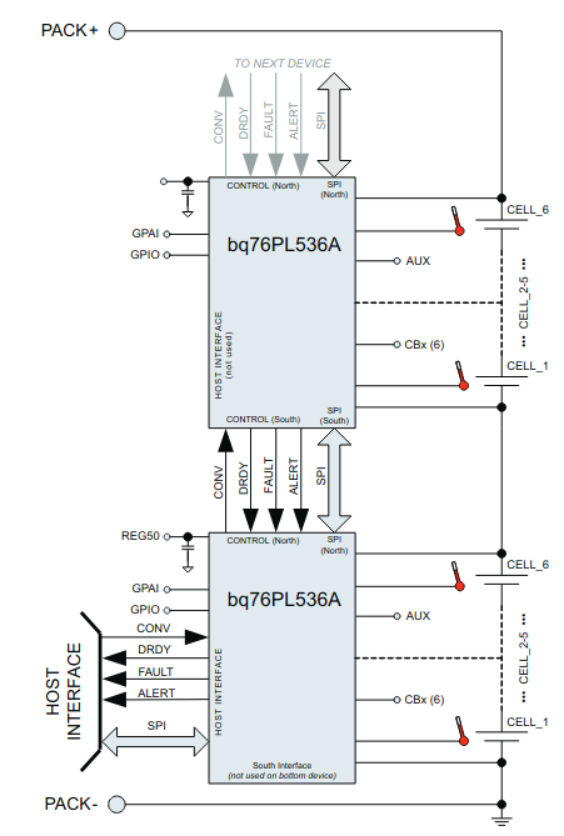
\includegraphics[width=0.8\textwidth]{bq76_simplified_schematic.png}
        \caption{Esquem\'atico simplificado de un balanceador de m\'as de 6
        celdas utilizando varios BQ76PL536A acoplados entre s\'i.}
        \label{bq76_simplified_schematic}
    \end{center}
\end{minipage}

\subsubsection{Diseño e Implementación}

En primer instancia, al tener que controlar solo un pack de bater\'ias de 6
celdas, solo se utiliz\'o un solo \acrshort{IC} sin necesidad de acoplar otro
integrado similar para extender su capacidad, esto se puede observar en la
Figura \ref{fig:bq76_implementation_sch}, en la que se muestra la implementaci\'on del
dispositivo, donde el puerto SPI norte est\'a conectado a la tensi\'on total del 
pack de bater\'ias ($\mathrm{V_{BATT}}$) y el puerto sur a masa 
($\mathrm{GND}$), anulando ambos perif\'ericos.

En la Figura \ref{fig:bq76_implementation_uncouple} se muestran todos los capacitores de desacople
especificados por el fabricante \cite{BQ76PL536A}:

\begin{itemize}
    \item $\matrhm{V_{REF}}$ y AGND requieren un capacitor de 10uF de
        desacople conectados entre ellos lo m\'as cerca posible a esos pines.
    \item La fuente anal\'ogica interna tiene que ser bypasseada a trav\'es del
        pin LDOA con un capacitor cer\'amico de 2.2uF.
    \item La salida del regulador de 5V que provee el integrado (REG50) tiene 
        que ser filtrado con un capacitor de 2.2uF, independientemente de si 
        esta fuente es utilizada o no externamente.
\end{itemize}

\begin{figure}[!h]
    \begin{subfigure}[b]{\textwidth}
        \begin{center}
            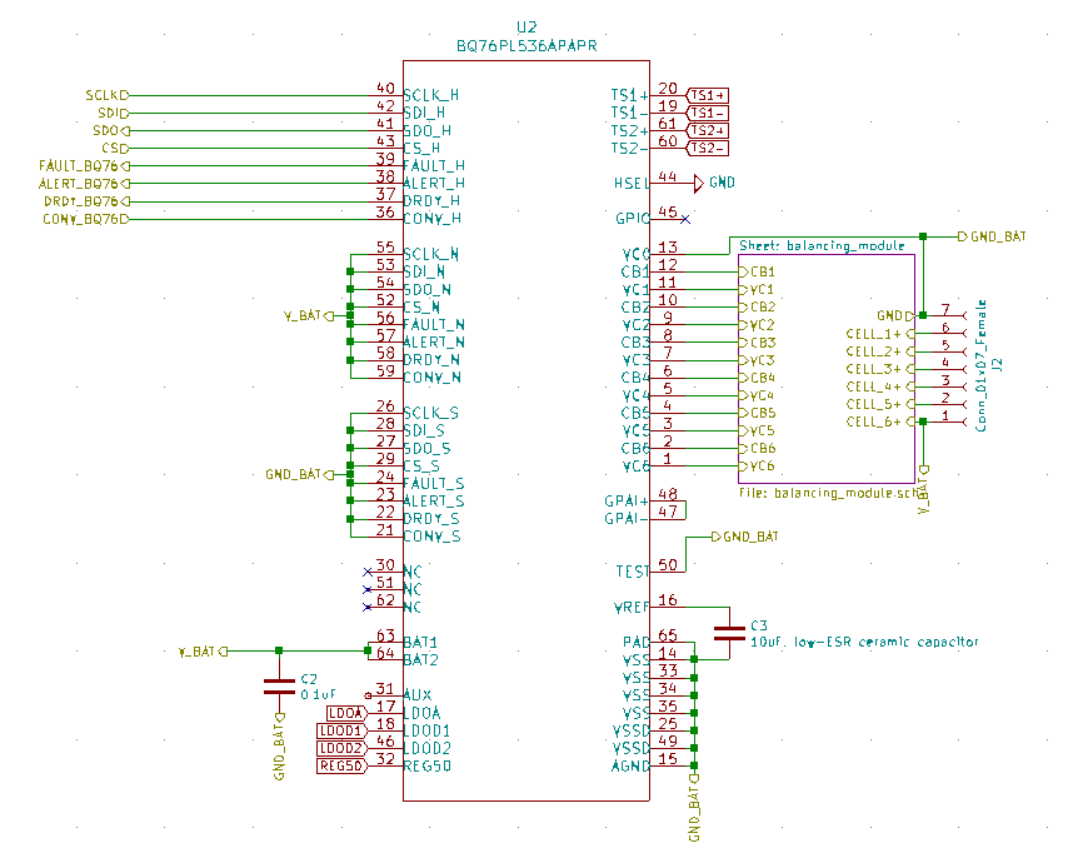
\includegraphics[width=0.95\textwidth]{bq76_implementation.png}
            \caption{Esquem\'atico diseñado del BQ76PL536A}
            \label{fig:bq76_implementation_sch}
        \end{center}
    \end{subfigure}

    \hfill{3mm}

    \begin{subfigure}[b]{\textwidth}
        \begin{center}
            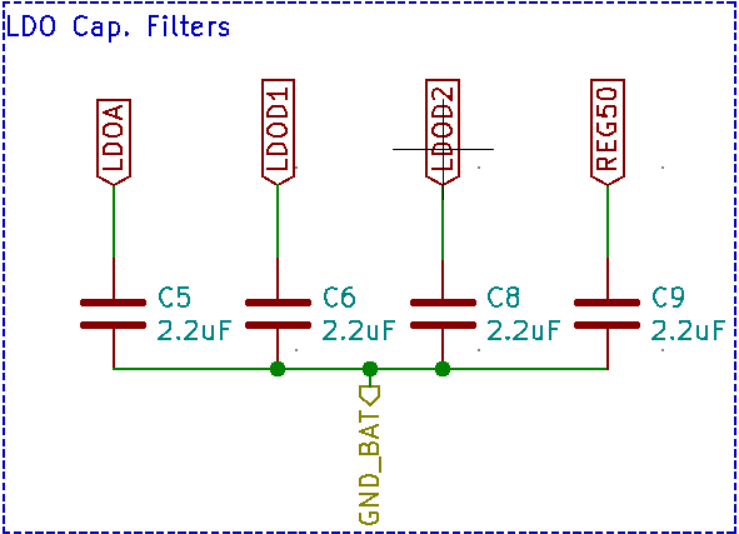
\includegraphics[width=0.35\textwidth]{bq76_desacople.png}
            \caption{Capacitores de desacople requeridos para el correcto
            funcionamiento del \acrshort{CI}}
            \label{fig:bq76_implementation_uncouple}
        \end{center}
    \end{subfigure}
            \caption{Diseño implementación BQ76PL536A}
            \label{fig:bq76_implementation}
\end{figure}

El \acrshort{CI} bq76PL536 posee 6 salidas dedicadas, del pin CB1 a CB6, los
cuales funcionan como driver de control de los transistores N-FETs utilizados
como llaves para balancear las celdas correspondiente a cada una de las series
del pack de batería.
Por cada grupo de celdas en serie del pack de baterías se implemente un circuito
equivalente al de la Figura \ref{fig:bq76_balance_power}, encargado de manejar
la potencia de descarga del balanceo de las celdas.
El circuito de balanceo consta de un transistor N-FET \textbf{2N7002} de la
firma \emph{ON Semiconductors} en su empaquetado SOT−23 junto con las
resistencias R15, R18 y el diodo D1 que forman parte del curcuito de encendido
del Mosfet. 
%TODO: Por que seleccionamos el 2N7002
Y una resistencia, R21 en el caso del ejemplo presentado en la
Figura \ref{fig:bq76_balance_power}, que hace las veces de carga según se
describio en la sección \ref{} respecto del método de balanceo seleccionado. 

La implmentación del algoritmo de balanceo apropiado es implementado y procesado
en la unidad de procesamiento del \acrshort{BMS}.  

%TODO: corriente de descarga por celda

\begin{figure}[!h]
    \begin{center}
        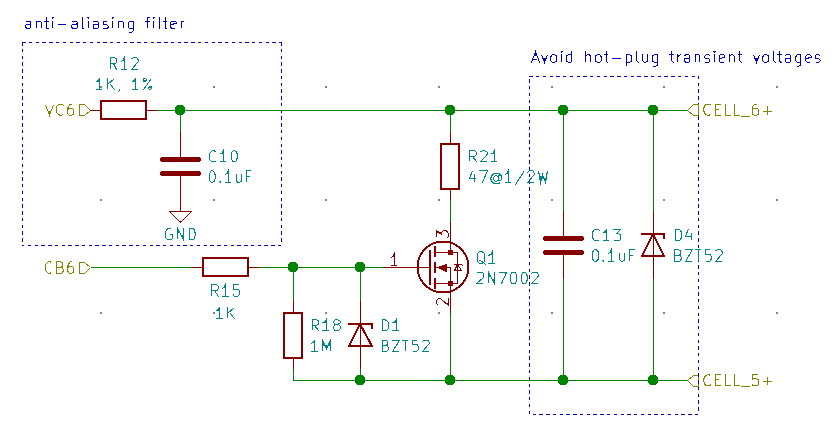
\includegraphics[width=0.7\textwidth]{hardware/bat_monitor/bat_mon_balance.png}
        \caption{Módulo balance BQ76PL536A}
        \label{fig:bq76_balance_power}
    \end{center}
\end{figure}

%Todo: anti-aliasing filter

%TODO: Avoid- hot-plug- transientes voltages
\newpage

\subsection{Sensor de corriente}

\subsubsection{Tecnología Seleccionada - INA226}

Frente a los requerimientos y la naturaleza de un \acrshort{BMS} se ha
seleccionado la tecnología de sensado de corriente por resistencia Shunt.
Actualmente existen en el mercado un sin número de soluciones de amplificadores
y moduladores aislados que permiten alcanzar precisas mediciones de corrientes
con este método, logrando as\'i minimizar las injerencias del entorno siempre 
y cuando se seleccione una resistencia Shunt adecuada y el diseño del circuito
impreso (\acrshort{PCB}, del ingl\'es \emph{\acrlong{PCB}}).

\noindent Las ventajas de la medición a partir del método de resistencia 
shunt son:

\begin{itemize}
    \item Bajo offset y baja susceptibilidad frente a influencias de campos 
	magnéticos externos y variaciones de temperatura.
    \item Alta linealidad de la solución en todo el rango de voltaje en 
	comparación a la solución basada en tecnología Hall, sobre todo en 
	la zona cercana a cero y la de saturación del nucleo. 
    \item Mejor resolución para mediciones de corriente continua frente a 
	las soluciones basadas en mediciones de efecto Hall. 
	Particularmente debido a la baja sensitividad que presenta frente a 
	las influencias de los campos magnéticos externos.
    \item Pueden soportar operaciones en ambientes de altas temperaturas 
	manteniendo la linealidad debido a su bajo TCR. 
	Los sensores de efecto Hall encuentran su rango de operación 
	fuertemente acotado.
    \item Facilidad que presenta la tecnología para la integración en 
	circuitos impresos priorizando el tamaño reducido.
    \item Disponibilidad en distribuidores nacionales
\end{itemize}

\noindent El integrado propuesto para el sensado de corriente es el INA226 de
Texas Instruments. Seg\'un su hoja de datos \cite{ina226} el INA226 es un 
conversor analógico digital de 16 bits (ADC) que implementa una interfaz 
compatible I2C para la comunicación con el módulo del control. El dispositivo 
monitorea simultaneamente la tensión que cae en una resistencia shunt y la del 
bus de alimentación. Permite múltiples calibraciones y seteos, entre ellos 
variar los tiempos de conversión y definir conversiones múltiples que al 
implementar internamente un multiplicador y divisor permite obtener lecturas 
directas de tensión y potencia en amperes y en Vatios.

En la Figura \ref{fig:ina226-commonimplementation} se puede observar su 
implementación modelo. 

\begin{figure}[h!]
    \begin{center}
	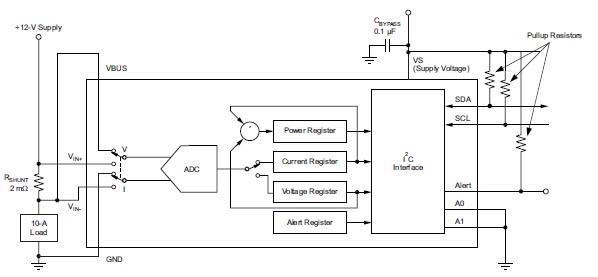
\includegraphics[width=0.7\linewidth]{assets/INA226-Common_Implementation}
	\caption{Implementación Tipo - INA226}
	\label{fig:ina226-commonimplementation}
    \end{center}	
\end{figure}
\FloatBarrier

\subsubsection{C\'aculo de la resistencia shunt}

Para realizar el c\'aculo de la resistencia shunt utilizada para el sensor de
corriente, se debe tener en cuenta el rango de voltaje de entrada que
especifica la hoja de datos del dispositivo INA226 y las caracter\'isticas del
pack de bater\'ias descripto en la Secci\'on \ref{caract_pack}. 

En este caso, se busca medir una corriente m\'axima de 20A con el objetivo de
tener un margen de medici\'on de corriente mayor al m\'aximo permitido para la
circulaci\'on del pack. Entonces, teniendo en cuenta el rango del voltaje de
la resistencia shunt en el INA226 \emph{(Ec. \ref{v_range_shunt})} y la ley de
Ohm \emph{(Ec. \ref{ohm_law})}:

\begin{equation}
    -81.9175mV \le V_{shunt} \le 81.92mV  \label{v_range_shunt}
\end{equation}

\begin{equation}
    V=I \times R \label{ohm_law}
\end{equation}

el valor m\'aximo de la resistencia Shunt es de \textbf{4,096m$\Omega$}. Por el
otro lado, tambi\'en se debe tener en cuenta la potencia m\'axima disipada por
la resistencia, cuyo c\'alculo es realizado por la Ecuaci\'on 
\ref{calc_pot_res},

\begin{equation}
    P_{disipada} = V \times I = I^2 \times R = \frac{V^2}{R} \label{calc_pot_res}
\end{equation}

dada la corriente m\'axima a medir y la tensi\'on m\'axima de lectura, la
potencia m\'axima disipada por la resistencia shunt es de 1,64W. Por lo tanto,
la resitencia shunt est\'a dada por las siguientes caracter\'isticas:

\begin{itemize}
    \item Resistencia m\'axima de $4.096m\Omega$.
    \item Potencia m\'axima disipada de 1.64W.
\end{itemize}

Teniendo en cuenta la disponibilidad del mercado local, se elije una resistencia 
de $2.5m\Omega$ apta para disipar una potencia m\'axima de 1W de montaje
superficial (\acrshort{SMT}, del ingl\'es \acrlong{SMT}) tipo 2512 
(25 pulgadas de largo, 12 pulgadas de ancho), esto permite realizar una
medici\'on m\'axima de 20A pero desaprovechando el rango m\'aximo del INA226 en
la medici\'on de voltaje sobre la resistencia shunt, ya que la tensi\'on
m\'axima que se refleja sobre al resistencia es de $\mathrm{\pm}$50mV.

\subsubsection{Esquem\'atico del circuito}

El esquem\'atico del circuito se puede observar en la Figura \ref{ina226_sch}.

\begin{figure}[h!]
    \begin{center}
        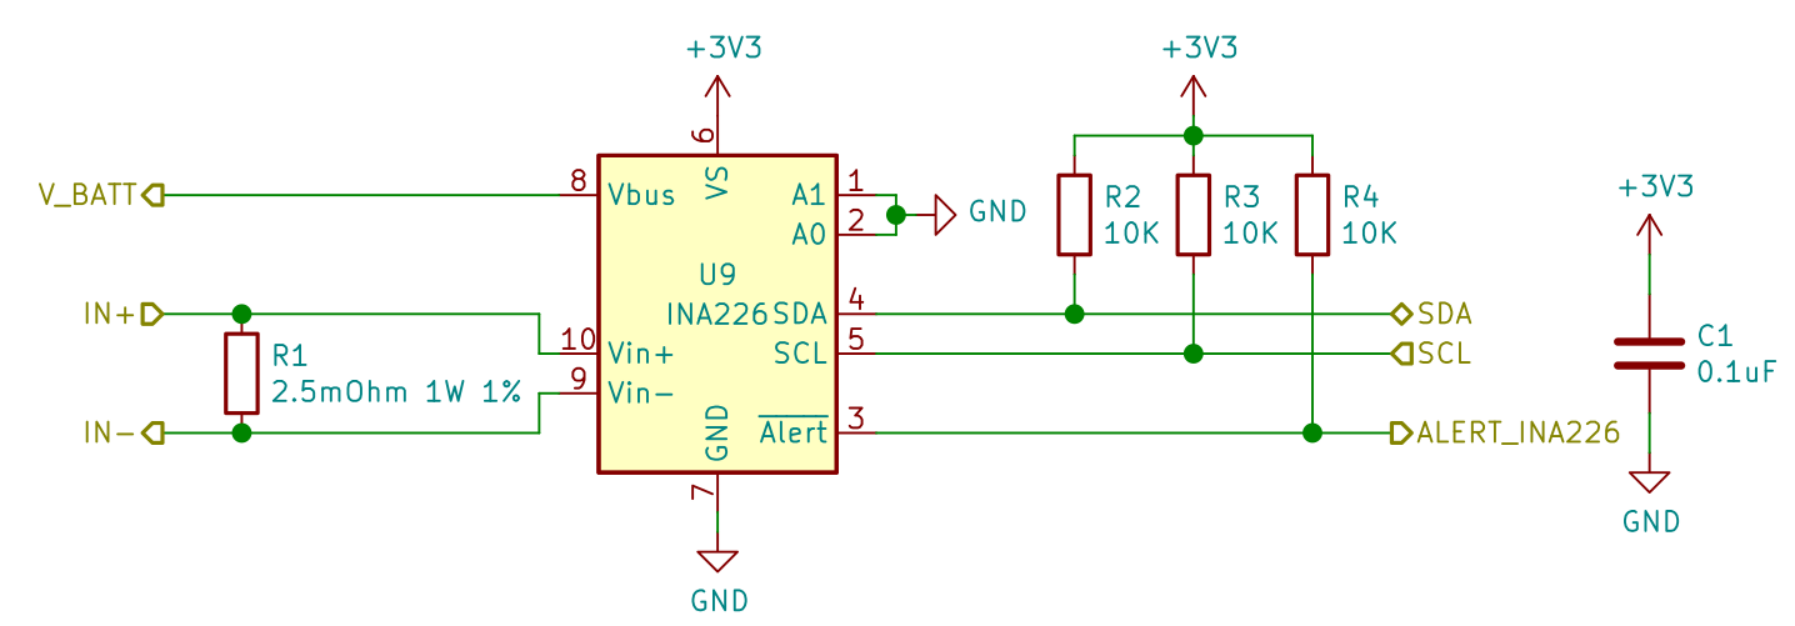
\includegraphics[width=0.8\textwidth]{ina226_sch.png}
        \caption{Esquem\'atico del sensor de corriente implementado en el diseño
                 final}
        \label{ina226_sch}
    \end{center}
\end{figure}

En el mismo, R1 se corresponde con la resistencia shunt, mientras que R2, R3 y
R4 son resistencias de pull necesarias por el protocolo de comunicaci\'on I2C.
Por el otro lado, el capacitor C1 act\'ua como capacitor de desacople.

\subsection{Interruptor de desconexión entre batería y el Vehículo}

Uno de los objetivos principales del BMS es el de garantizar la seguridad del
pack, del usuario y del vehículo eléctrico. Para tal propósito el sistema debe
contar con un interruptor que permita a la batería salir de servicio si las
condiciones de seguridad no se cumplen en su totalidad.

Para el diseño del interruptor se tiene en cuenta las características del
sistema las cuales son:

\begin{itemize}
	\item Tensión de bloqueo = 25V
	\item Corriente Máxima = 15A
\end{itemize}

\subsubsection{Caracteristicas de un MOSFET en conmutación}

Si bien los dispositivos semiconductores de potencia generalmente son modelados
como interruptores ideales, los mismos poseen características que los dista de
la perfección, como lo son las resistencias intrínsecas, capacidades parásitas,
etc.

Por estas caracteristicas los tiempos de apagado y encendido o tiempos de
conmutación no son nulos y se tienen que tener en cuenta en aplicaciones de alta
frecuencia.Si bien la aplicación en particular no es de alta frecuencia, se
propone minimizar el tiempo de apagado para que la desconexión de la batería y
la carga sea prácticamente instantanea y lleve al sistema a un estado de
seguridad rapidamente evitando así posibles daños en el equipo.

Los transistores que funcionan como interruptores trabajan principalmente en 2
estados, en conducción y en corte (particularmente los mosfet en región
\'ohmnica y región de corte),al conmutar, sin embargo, se pasa brevemente por el 
estado de saturación por lo que se debe tener en cuenta para entender los 
fenómenos asociados a los tiempos de apagado y encendido.

Para analizar el comportamiento durante la conmutación se debe tener en cuenta
los modelos en los estados por los cuales transiciona el transistor, los mismos
se muestran en la figura \ref{modelo_mosfet}. 

\begin{figure}[h!]
	\begin{center}
		\begin{minipage}[c]{0.95\textwidth}
			\centering
			\begin{circuitikz}[american]
				%Zona ohmnica
				\draw (7,2) 	to [short,-*]					(7,2.4) node[above] {D};
				\draw (5,2)	to [short]							(7,2);
				\draw (7,2) 	 -- 							(7,1);
				\draw (7,1) 	to [R,l=$R(V_{GS})$] 			(7,-1);
				\draw (5,0) 	to [C = $C_{GD2}$]   			(5,2);
				\draw (5,-2) 	to [C = $C_{GS}$]				(5,0);
				\draw (4.5,0) 	node[above] {G} to [short,*-]	(5,0);
				\draw (7,-1)    to [short,-*] 					(7,-2.4)node[below] {S};
				\draw (5,-2)   to [short] 						(7,-2);
				
				%Zona saturación
				\draw (0,2) 	to [short,-*]					(0,2.4) node[above] {D};
				\draw (-2,2)	to [short]						(0,2);
				\draw (0,2) 	 -- 							(0,1);
				\draw (0,1) 	to [isource,l=$I(V_{GS})$] 		(0,-1);
				\draw (-2,0) 	to [C = $C_{GD1}$]   			(-2,2);
				\draw (-2,-2) 	to [C = $C_{GS}$]				(-2,0);
				\draw (-2.5,0) 	node[above] {G} to [short,*-]	(-2,0);
				\draw (0,-1)    to [short,-*] 					(0,-2.4)node[below] {S};
				\draw (-2,-2)   to [short] 						(0,-2);
			\end{circuitikz}
		\end{minipage}
	\end{center}
	\caption{Modelos de transistor mosfet en zonas de saturación y ohmnica respectivamente.}
	\label{modelo_mosfet}
\end{figure}
\FloatBarrier

Por otro lado, respecto a las capacidades intrínsecas del transistor se sabe que
la capacidad de \emph{gate-source} $C_{GS}$ tiene el mayor valor, y es
prácticamente constante ya que queda determinada por la geometría del
\emph{gate} y la metalización del \emph{source}.

La capacidad de \emph{gate - drain}  $C_{GD}$ es la capacidad entre el
\emph{gate} y la zona n- conductora fuera de la zona de deplexión formada por la
polarización directa \emph{drain-source}. El dieléctrico de esta capacidad es la
zona de óxido y la zona empobrecida de portadores contigua a la zona del
\emph{gate-source}, aproximandose al valor de $C_{GS}$ cuando $V_{DS}= 0V$ y
disminuyendo rápidamente con $V_{DS}$ creciente. Con tensión $V_{DS}$ del orden
de la tensión $V_{GS}$ de comando del MOSFET (10-15V) la capacidad es
aproximadamente 30 veces menor  que con $V_{DS}\approx1V$. Para efectos de
estudiar la conmutación la capacidad $C_{GD}$ puede modelarse como en la figura
\ref{aprox_CGD}.

Se asume que $C_{GD}$ tiene valor $C_{GD1}$ para tensiones de $V_{DS}$ mayores
que la tensión de comando de \emph{gate}, $V_{gg1}$, (llave todavía abierta) y
un valor $C_{GD2}$ mucho mayor para tensiones menores que $V_{GS}$ de comando
(llave cerrándose)\cite{Mohan1989}.

\begin{figure}[h!]
	\begin{center}
		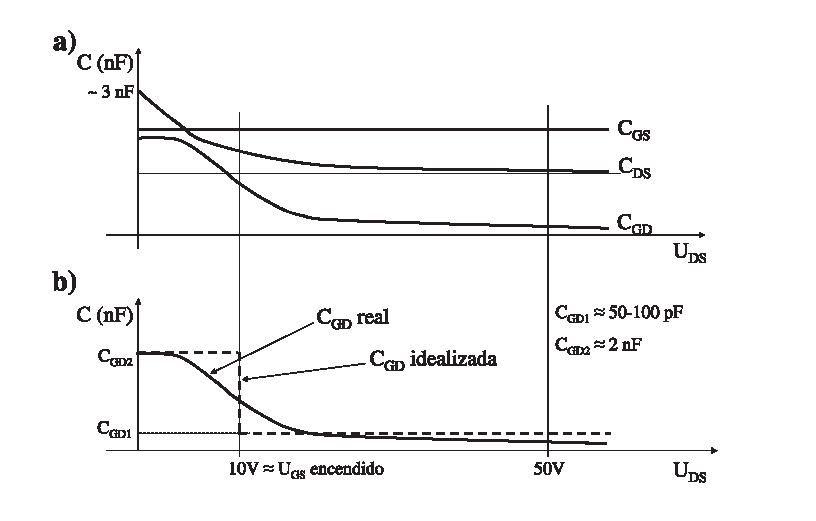
\includegraphics[width=0.75\textwidth]{Capacitor_vs_Vds.pdf}
		\caption{Variación de las capacidades del MOSFET en base a $V_{DS}$.}
		\label{aprox_CGD}
	\end{center}
\end{figure}
\FloatBarrier

\subsubsection{Análisis del tiempo de apagado}

Teniendo en cuenta el punto anterior y que la carga es un motor, por ende de 
caracter inductivo, surge la necesidad de realizaer el siguiente análisis sobre 
el circuito de la Figura \ref{comando_mosfet}:

\begin{figure}[h!]
	\begin{center}
		\begin{minipage}[c]{0.7\textwidth}
			\centering
			\begin{circuitikz}[american]
				%\draw[step=0.5,green,thin,xshift=0.5cm,yshift=0.5cm] (-6,-6) grid (6,6);
				\draw (0,5)	to [short]						(1.5,5);
				\draw (0,2.4)	to [short]						(1.5,2.4);
				\draw (0,5) 	to [short,-o]				(0,6) node[above] {$V_{bat}$};
				\draw (0,5) 	to [isource,l=$I_0$] 			(0,2.4);
				\draw (1.5,2.4)		to [diode]						(1.5,5);
				%Transistor
				\draw (0,2) 	to [short,-*]					(0,2.4) node[left] {D};
				\draw (-2,2)	to [short]						(0,2);
				\draw (0,2) 	 -- 							(0,0.75);
				\draw (0,0.27) 	node[nigfete]{};
				\draw (-2,0)	to [short]						(-0.95,0);
				\draw (-2,0) 	to [C = $C_{GD}$]   			(-2,2);
				\draw (-2,-2) 	to [C = $C_{GS}$]				(-2,0);
				\draw (-2.5,0) 	node[above] {G} to [short,*-]	(-2,0);
				\draw (0,-0.5)  to [short,-*] 					(0,-2.4)node[left] {S};
				\draw (0,-2.4)  to (0,-3) 						node[ground]{};
				\draw (-2,-2)   to [short] 						(0,-2);
				
				\draw (-2.5,0)  to [R =$ $]					(-4,0);
				\node (RG) at (-3.25,0.5){$R_g$};
				\draw (-4,0) 	to [short,-o]				(-4.5,0) node[above] {$V_{gg}$};
				
				\draw (-0.5,0) to[open, v=$V_{GS}$] (-0.5,-2);
				\draw (0.5,1) to[open, v=$V_{DS}$] (0.5,-1);
			\end{circuitikz}
		\end{minipage}
	\end{center}
	\caption{Modelos de transistor mosfet en conmutación clampeado por carga inductiva y diodo de freewheeling.}
	\label{comando_mosfet}
\end{figure}
\FloatBarrier

En condiciones de conducción $V_{DS}\approx 0V$, siendo $I_0$ la corriente de la
carga en el momento de la conmutación, la tensión $V_{DS}$ es estrictamente
$R_{ds(ON)}I_0$  y $V_{GS}=V_{on}$.

En el momento que $V_{gg}$ pasa de $V_{on}$ a $0V$ las capacidades $C_{gs}$ y
$C_{gd}$ comienzan a descargar a través de $R_g$ con una evolución exponencial
con $\tau_1 = R_g (C_{gd2}+C_{gs})$. $C_{gd}$ en este momento posee su mayor
valor ya que $V_{DS}$ es muy baja.

Esta evolución es cursada hasta que $V_{gs}$ alcanza el valor umbral $V_{gsa}$,
este valor cumple con la condición $I_D(V_{gsa})=I_0$.

A partir de aquí, $V_{DS}$ comienza a aumentar, mientras $C_{gd}$ se carga
linealmente con corriente $I_g=V_{gsa}/R_g$ en principio con pendiente baja
$I_g/C_{gd2}$ y para $V_{ds} > V_{gg1}$, siendo $V_{gg1}$ el valor umbral
mencionado en \ref{aprox_CGD}, con pendiente más alta $I_g/C_{gd1}$.

Es fundamental destacar que la corriente $I_g$ impacta directamente sobre los
tiempos de apagado, por lo que generalmente se utiliza una resistencia de
apagado $R_g$ menor para minimizar el tiempo de apagado del dispositivo.

Por último, cuando $V_{DS} = V_{bat} + V_{diodo-on} $ el diodo de
\emph{freewheel} comienza a conducir y la corriente de $I_D$ comienza a
disminuir, momento en el cual $C_{gs}$ comienza a descargarse a través de $R_g$
con $\tau_2 = R_g (C_{gd1}+C_{gs})$ hasta que $V_{ds}$ alcanza el valor $V_T$ e
$I_D = 0A$, $V_{gs}$ continúa decayendo hasta $0V$. Todo este proceso se puede
observar temporalmente en la Figura \ref{apagado_time}.

\begin{figure}[h!]
	\begin{center}
		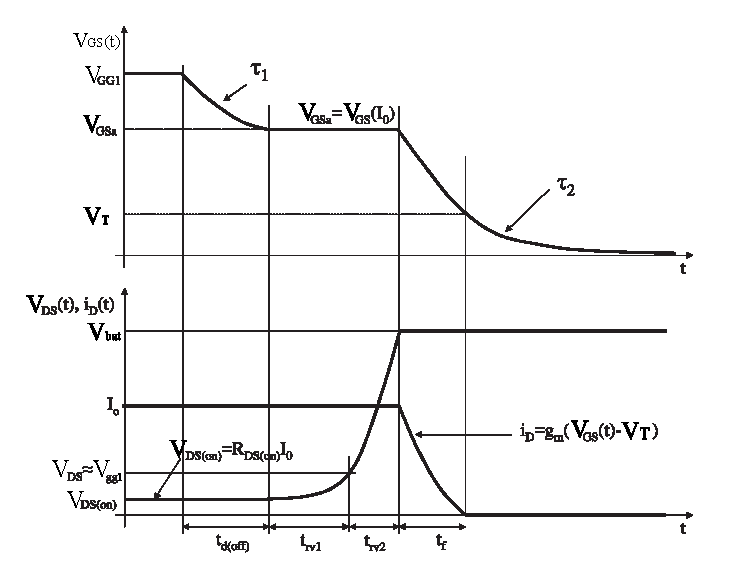
\includegraphics[width=0.75\textwidth]{shutdown_time.pdf}
		\caption{Evolución temporal del apagado de un MOSFET.}
		\label{apagado_time}
	\end{center}
\end{figure}
\FloatBarrier

Los interruptores pueden ser clasificados, según su interconexión respecto a la
carga y la alimentación, como \emph{high side} o \emph{low side} drivers. 
La diferencia principal radica en que el primero desconecta la
carga del borne de mayor potencial de la batería, el positivo, y el otro
desconecta la carga del borne de menor potencial, el negativo. La figura
\ref{low_high_driver_sch} muestra los dos tipos de interruptores implementados
con transistores mosfet.

Los interruptores de tipo \emph{low-side} son generalmente utilizados en cargas
asociadas a la transmisión de movimiento, como lo son los motores, también
solenoides y calentadores. Por otro lado, los interruptores de tipo
\emph{high-side} son utilizados en bombas de combustible y componentees
asociados a la carrocería como asientos, iluminación, limpiaparabrisas y
ventiladores \cite{DigKey2016}.

Estos interruptores difieren principalmente con respecto a su respuesta ante
fallas. Es más probable encontrar fallas de cortocircuito a masa que
cortocircuitos a la alimentación, dado que el chasis integro del vehiculo esta
conectado a masa. Para un interruptor \emph{low-side} un cortocircuito a masa
provoca el encendido de la carga. Para el caso del \emph{high-side} un
cortocircuito en su salida generará una sobrecorriente en el interuptor por lo
que se deben tener en cuenta protecciones para el interruptor.

Para la condición opuesta (cortocircuito a la alimentación) los comportamientos
se invierten.

Esta diferencia es la que determina el uso de uno u otro interruptor, un ejemplo
de esto es ante un accidente, si la bomba de combustible es conectada mediante
un interruptor a masa, es probable que haya un cortocircuito a masa y se
encienda, lo que potencialmente causaría consecuencias catastróficas.

\begin{figure}[h!]
	\begin{center}
		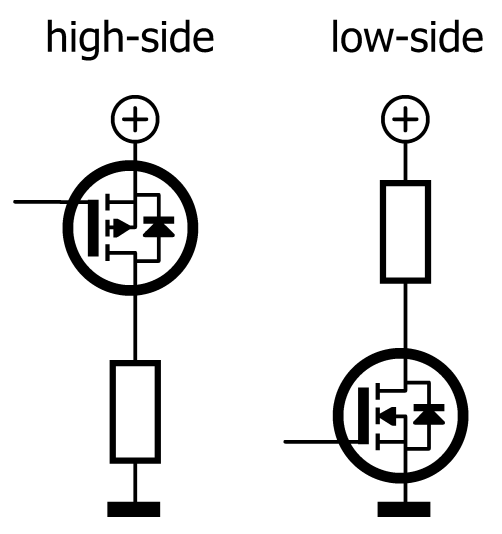
\includegraphics[width=0.30\textwidth]{low_high_driver_sch.png}
		\caption{Esquema interruptor a masa e interruptor a positivo.}
		\label{low_high_driver_sch}
	\end{center}
\end{figure}
\FloatBarrier

Para la implementación del sistema se optó implementar un \emph{high-side
driver} con un transistor IRF9310PbF de Infineon Technologies, el cual posee una
tensión de bloqueo de $30V$ y una corriente máxima de drain de $20A$, pero la
característica fundamental es que a pesar de ser un MOSFET canal P posee un
valor de $R_{on}=4.6 m\ohm$ minimizando perdidas en conducción. El circuito de
la figura \ref{load_sw_sch} posee una etapa de adaptación para conectar la
salida del microcontrolador al gate del interruptor y un circuito de apagado
rápido para incrementar la corriente de gate y minimizar el tiempo de apagado.

\begin{figure}[h!]
	\begin{center}
		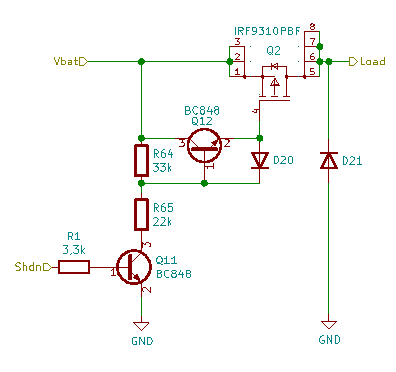
\includegraphics[width=0.6\textwidth]{kcd_bat_load_switch.pdf}
		\caption{Circuito Interruptor carga-batería}
		\label{load_sw_sch}
	\end{center}
\end{figure}
\FloatBarrier

El IRF9310PbF adquiere el menor valor de $R_{DS(on)}$ cuando $V_{gs} = 10V$
según la hoja de datos\cite{IRF9310}, mientras que la tensión que soporta
$V_{gs-max}=20V$ por lo que en conducción se calculan $R_{64}$ y $R_{65}$ para
$V_{gs}=15V$.
Además, se busca minimizar el consumo del circuito ya que la autonomía del
vehículo puede verse afectada si no se tiene en cuenta.

$R_1$ simplemente debe cumplir la relación $I_b = I_{R1} \beta >> I_d = I_{R65}
= I_{R64}$, Para asegurar la saturación de $Q_{11}$. 

Para el apagado del transistor surge la necesidad de agregar el transistor
$Q_{12}$ ya que al abrirse $Q_{11}$ la capacidad $V_{gs}$ busca descargarse a
través de $R_{64}$ la cual es de un valor alto para minimizar las perdidas en
conducción para mantener $V_{gs}=-15V$. La función de este transistor, $Q_{12}$
en conjunto con $D_{20}$ es la de cortocircuitar $V_{gs}$ de manera de reducir
la resistencia vista y minimizar el tiempo de apagado sin impactar en el consumo
pasivo del dispositivo.

Por último se agregó $D_{21}$ como diodo de \emph{freewheel}.

\subsection{Circuito Cargador de Batería}

\subsubsection{Tecnología Seleccionada - TI bq24610}

Para lograr un completo control del perfil de carga descripto en la 'Sección'
\ref{sec:tecnica_carga}  es que seleccionamos e implementamos el circuito
integrado \emph{bq24610} de la firma \emph{Texas Instrument}.

El \emph{bq24610} es un circuito altamente integrado que implementa un cargador
de \acrfull{Ion-Li} o \acrfull{Li-Po} capaz de operar de forma independiente o
stand-alone.

Implementa un convertirdor de energía DC-DC del tipo buck sin aislamiento que
nos permite obtener un perfil de tensión y corriente controlado como el
descripto en la sección \ref{sec:tecnica_carga} a partir de una fuente de
alimentación de tensión continua externa.

Emplea un controlador de corriente y de tensión sincrónico
switching PWM de frecuencia constante y de alta resolución cuya
topología simplificada puede observarse en la figura \ref{fig:simp_sch_char}. 

\begin{figure}[h!]
    \centering
    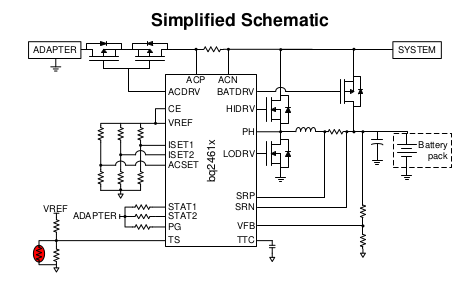
\includegraphics[width=0.5\textwidth]{bat_char/simp_sch_char.png}
    \caption{Esquema simplificado Cargador de Batería}
    \label{fig:simp_sch_char}
\end{figure}
\FloatBarrier

Admite la conexión de hasta 6 celdas en serie con una tensión y
corriente máxima de entrada de hasta $28V$ y $10A$ respectivamente y una salída
de hasta $26V$ y $10A$ ajustandose adecuadamente a nuestros requerimientos y a
la topología de nuestro pack de baterías \emph{6S3P} descripta en \ref{batSel}.
El empaquetado del mismo es del tipo VQFN.

%\noindent Como se comentó en secciones anteriores, cuando múltiples celdas se
%encuentran conectadas en serie, el voltaje de una celda no siempre coincide con
%la tensión equivalente del pack de baterías dividido por el número de celdas. 
%
%\noindent La ecualización de celdas es una técnica en la cual se trata de
%mantener los niveles de voltaje entre las celdas que conforman la cadena
%conectada en serie de un pack de baterías de forma homogénea, es decir, que los
%niveles de tensión entre celdas sea lo más uniforme posible, con el objetivo de
%maximizar la eficiencia del pack de baterías.
%
%\noindent El desbalance más típico generalmente se manifiesta en una variación
%en el voltaje entre éstas, que puede ser corregido instantáneamente o
%gradualmente conectando cargas externas en paralelo, a través de sus
%correspondientes transistores, provocando una corriente de descarga adicional
%que pueden ir desde miliamperes hasta varios Amperes, dependiendo del
%dimensionamiento energético del pack de baterías. Sin embargo, este desbalance
%en tensión es, por lo general, dado por desbalances químicos o distintas
%dinámicas de descarga entre celdas, provocando que el objetivo del balanceo no
%esté claramente definido provocando más perjuicios que beneficios al sistema
%completo.  De hecho, la mayoría de las metodologías basadas en el desbalance de
%voltaje, llevan a un pack de baterías más desbalanceado que sin ellos.

\subsubsection{Diseño e Implementación}

La sección describe la implementación y desarrollo de un circuito cargador de
baterías de Ion-Litio a partir del \acrfull{CI} bq24610 de la firma Texas
Instruments implementado en nuestro \acrshort{BMS}.

Se describen sus partes fundamentales y se presentan los cálculos realizados y
los criterios tenidos en cuenta para la selección de los componentes. 

\begin{figure}[h!]
    \centering
    \begin{subfigure}[t]{0.6\textwidth}
        \centering
        \includegraphics[width=1.1\textwidth]{hardware/bat_charger/bc_ic.png}
        \caption{Implementación bq24610 Texas Instrument}
        \label{fig:bc_ic_ti}
    \end{subfigure}
    \hfill
    \begin{subfigure}[t]{0.35\textwidth}
        \centering
        \includegraphics[width=0.9\textwidth]{hardware/bat_charger/bc_ic_power_supply.png}
        \caption{Alimentación bq24610}
        \label{fig:bc_ic_power_supply}
    \end{subfigure}
    \caption{Implementación Cargador de Batería de Ion-Li bq24610 de TI}
    \label{fig:bc_ic}
\end{figure}
\FloatBarrier

Las condiciones de operación que sirvieron como parámetros de diseño son las
siguientes:

\begin{tabular}{ll}
    $V_{In}=28V$ &Tensión de alimentación \\
    $V_{Out (max)}=25.2V$ &Tensión de salida máxima\\
    $V_{Out (min)}=18.6V$ &Tensión de salida mínima\\
    $I_{Out (max)}=5A$ &Corriente de salida máxima\\
    $V_{DS (on)}=37.55mV$ &Caida de voltaje en elemento switching Q9\\
    $f_{s}=600 KHz$ &Frecuencia switching\\
\end{tabular}

\subsubsubsection{Alimentación}

El circuito de alimentación del cargador de batería consta de una red de descarga
RC, de dos Mosfets canal-P colocados en configuración back to back con el objeto de
aislar la fuente de alimentación externa del circiuto del cargador propiamente
dicho y de una resistencia shunt de sensado de la corriente de entrada. 

\begin{figure}[h!]
    \begin{center}
	\includegraphics[width=0.6\textwidth]{hardware/bat_charger/bc_input.png}
	\caption{Entrada de alimentación externa}
	\label{fig:cb_input}
    \end{center}
\end{figure}
\FloatBarrier

Los mosfets Q7 y Q8 colocados entre la fuente de alimentación y el \acrshort{CI}
previene que fluya una corriente inversa de descarga desde el pack de baterías
en caso de que se encuentren apagados y minimizan la disipación de energía a
partir de la baja resistencia $R_{DS(on)}$ que presentan operando en directa, en
comparación a un diodo Schottky. Q8 a su vez provee al circuito la capacidad de
variar la corriente de alimentación de forma controlada $di/dt$ al conectar la
fuente de alimentación al circuito mediante el control del tiempo de encendido.
    
Durante una conexión o desconexión en caliente de la fuente externa de
alimentación, la presencia de picos de sobre voltaje en la entrada pueden
afectar al \acrshort{CI}. Esto se debe al sistema de segundo orden formado por
las inductacias y capacidades parácitas que pueden presentarse en el cable de la
fuente de alimentación. R38 y C24 en serie fornan un circuito de descarga que
elimina los picos de sobre tensión producidos por estos transitorios.

Se seleccionó un valor de resistencia snubber $R_{S}$ que, por lo menos, permita
la circulación de una magnitud de corriente equivalente a la de alimentación en
caso de una desconexión en caliente de la fuente de alimentación externa o de un
corte en los mosfet de entrada por parte del \acrshort{CI} siguiendo los
lineamientos en \cite{CD_RC_Snubber_AN}.  

\begin{align}
    R_{S} &\leq \frac{V_{In (max)+2V}}{I_{In (max)}}\\
    &=\frac{30V}{5A}\\
    &=6\ohm
\end{align}

La disipasión de energía en $R_{S}$ es independiente de su valor y de la
corriente circulante ya que disipa la energía almacenada en el capacitor snubber
$C_{S}$ en serie con la misma. Acorde a la potencia \emph{P} máxima admitida
por la resistencia R38 seleccionada, $1/4W$, calculamos una capacidad $C_{S}$. 

\begin{align}
    P&=\frac{C_{s}V_{In (max)}^{2}}{2}2f_{S'}\\
    &=C_{s}V_{In (max)}^{2}f_{s'}\\
    C_{s}&=\frac{P}{V_{In (max)}^{2}f_{S'}}\\
    &=2.6710nF
\end{align}
   
\subsubsubsection{Control de Perfil de Carga}

El perfil de carga \acrshort{CC} - \acrshort{CV} descripto en la sección
\ref{sec:tecnica_carga} y sus correspondientes parámetros de control se setean
en el bq24610 a partir de los divisores resistivos que se observan en la figura
\ref{fig:cb_set_point}.

\begin{figure}[h!]
    \centering
    \begin{subfigure}[t]{0.45\textwidth}
        \centering
        \includegraphics[width=0.75\textwidth]{hardware/bat_charger/bc_set_points_I.png}
        \caption{Circuito de fijación de Set-Point de corriente I}
        \label{fig:cb_set_point_I}
    \end{subfigure}
    \hfill
    \begin{subfigure}[t]{0.45\textwidth}
        \centering 
        \includegraphics[width=0.5\textwidth]{hardware/bat_charger/bc_set_points_v.png}
        \caption{Circuito de fijación de Set-Point de tensión V}
        \label{fig:cb_set_point_V}
    \end{subfigure}
        \caption{Fijación Set-Points del perfil de carga rápida}
        \label{fig:cb_set_point}
\end{figure}
\FloatBarrier

El set point de corriente del perfil de carga a corriente constante descripto en
la 'Sección' \ref{sec:tecnica_carga} es definido en el cargador de batería a
partir de fijar una tensión en ISET1, pin 11 del bq24610. El voltaje de
referencia se logra a partir de un divisor resistivo formado con R48 y R49 entre
$V_{ref} \equiv 3.3V$ y masa como se puede observar en la figura
\ref{fig:cb_set_point_I}. 

El voltaje aplicado en ISET1 define la corriente máxima de carga rápida, la cual
es sensada por la resistencia shunt de salida R52 ($R_{SR}$) conectada en
paralelo a SRP y SRN, pines 14 y 13 respectivamente del \acrshort{CI}.

La ecuación de corriente máxima de carga $I_{FastCharge}$ será entonces:

\begin{equation}
    I_{FastCharge}=\frac{V_{ISET1}}{20*R_{SR}}
    \label{eq:IFastCharge}
\end{equation}

Definiendo la corriente de salida máxima que puede entregar el cargador
$I_{Out (max)}=5A$ se selecciona el valor de la resistencia shunt sensora de la
corriente de salida $R_{SR}$. La diferencia de potencial máximo admitida entre
los pines SRP y SRN $\Delta V_{SR (Max)} \leq 100mV$.

\begin{align}
    R_{SR}&=\frac{I_{Out (max)}}{\Delta V_{SR (max)}}\\
    &=\frac{5A}{100mV}\\
    &=20m\ohm
\end{align}

El valor de $R_{SR}$ fue calculado con el objeto de que el circuito de sensado
de corriente de carga opere a fondo de escala a fin de maximizar la resolución
de la corriente de carga. 

Según la hoja de datos de la celda de litio NCR18650PF la corriente de
carga máxima de la misma debe ser 0.5 veces la capacidad nominal de la misma.
Debido a la configuración 6S3P de nuestro pack de batería con 3 celdas en
paralelo la corriente de carga rápida del mismo deberá ser fijada en $
I_{FastCharge}=0.5*C*3=4125mA$.

Despejando $V_{ISET1}$ de la ecuación \ref{eq:IFastCharge} se conoce el
valor de tensión que debemos aplicar en el terminal ISET1 del \acrshort{CI}.

\begin{align}
    V_{ISET1}&=I_{Fast_Charge}*20*R_{SE}\\
    &=4125mA*20*20m\ohm\\
    &=1.65v
\end{align}

A partir la tensión a aplicar en ISET1 se despejó el divisor resistivo para
conocer $R_{48}$ y $R_{49}$

\begin{align}
    V_{ISET1}&=V_{ref}*\frac{R_{49}}{R_{48}+R_{49}} \\
    V_{ref}*R_{49}&=V_{ISET1}*(R_{49}+R_{48}) \\
    \frac{(V_{ref}-V_{ISET1})*R_{49}}{V_{ISET1}}&=R_{48} \\
    R_{49}&=R_{48}
\end{align}

A los fines pŕacticos y evitando sobre cargar la salida de $V_{ref}$ del
\acrshort{CI} se adoptó $R_{48}$ y $R_{49}$ de $10K\ohm$ de 0.5\%

Si el pack de batería se encontrase profundamente descargado, el bq24610
aplicará una corriente de pre-carga. Este valor de corriente coincide con el de
corriente de fin de carga durante la fase de tensión constante del ciclo de
carga.

El set point de corriente de la pre-carga y de fin de carga se define en el
cargador de batería a partir de fijar una tensión en ISET2, pin 15 del bq24610.
El voltaje de referencia se logra a partir de un divisor resistivo formado
por $R_{50}$ y $R_{51}$ entre $V_{ref} \equiv 3.3V$ y masa. 

La ecuación de corriente de precarga $I_{pre charge}$ y de fín de carga $I_{cutt
off}$ será entonces:

\begin{equation}
    I_{cutt off}=I_{pre charge}=\frac{V_{ISET2}}{100*R_{SR}}
    \label{eq:ICutOff}
\end{equation}

Según la hoja de datos de la celda de litio NCR18650PF la corriente de cut-off o
fín de carga es 100mA a 25°C.  Por lo tanto, debido a la configuración 6S3P del
pack de batería con 3 celdas en paralelo la corriente de fin de carga sensada
por el cargador deberá ser 300mA.

Despejando $V_{ISET2}$ de la ecuación \ref{eq:ICutOff} se conoce  el valor de
tensión que deberá ser aplicado en ISET2.

\begin{align}
    V_{ISET2}&=I_{cutt off}*100*R_{SR}\\
    &=300mA*100*20m\ohm\\
    &=600mV
\end{align}

A partir de la tensión en ISET2 se despeja el divisor resistivo para conocer
$R_{50}$ y $R_{51}$

\begin{align}
    V_{ISET2}&=V_{ref}*\frac{R_{51}}{R_{50}+R_{51}}\\
    V_{ISET2}*(R_{50}+R_{51})&=V_{ref}*R_{51}\\
    \frac{(V_{ref}-V_{ISET2})*R_{51}}{V_{ISET2}}&=R_{50} \\
    \frac{9}{2}R_{51}&=R_{50}
\end{align}

Se adopta $R_{51} = 8K2\ohm$ y se calcula $R_{51} = 37K\ohm$, ambas resistencias
de 0.5\%

El set point de voltaje de carga propio del perfil de carga a voltaje contante
descripto en la 'Sección' \ref{sec:tecnica_carga} se define fijando una tensión en
VFB, pin 12 del bq24610. El voltaje de referencia es obtenido a partir de un
divisor resistivo formado por R55, R56 y R57, entre el voltaje del pack de
batería $V_{BAT}$ y masa como se observa en la figura \ref{fig:cb_set_point_V}. 

El voltaje aplicado en VFB es comparado al interior del \acrshort{CI} contra una
referencia de 2.05V la cual define si el voltaje de salida se haya por debajo o
por encima del valor deseado. 

La ecuación que define el voltaje de carga $V_{Charge} \equiv V_{VFB}$ será entonces:

\begin{equation}
    V_{Charge}=2.1V(1+\frac{R_{55}+R_{56}}{R_{57}})
\end{equation}

Según la hoja de datos de la celda de litio NCR18650PF el voltaje de carga de
una única celda es 4,2V a 25°C. Por lo tanto, debido a la configuración 6S3P del
pack de batería con 6 celdas en serie el voltaje de carga deberá ser fijado en
$V_{Charge} = 4.2V*6 = 25.2V$

A partir de conocer la tensión de carga $V_{Charge}$ se despejo el divisor
resistivo para conocer $R_{55}$, $R_{56}$ y $R_{57}$

\begin{equation}
	\frac{(V_{Charge}- 2.1)R_{57}}{2.1}=(R_{55}+R_{56})
\end{equation}

Se adoptó $R_{57}= 51K\ohm$ y se calculó $R_{55}+R_{56}=561K\ohm$, todas
resistencias de 0.1\% dado el orden de magnitud .

El divisor resistivo formado por R55, R56 y R57 se ubica en paralelo con la
batería. Es por esto que nos cercioramos que el drenado de corriente por el
mismo no descargue el pack de batería de forma incipiente. La corriente drenada
por el divisor es de $42\mu A=\frac{2900mAh}{42\mu A}*3=207142 hs \equiv 8630
dias$, tiempo que tardaría en descargar completamente el pack de batería.

El voltaje aplicado en ACSET, pin 16 del \acrshort{CI}, define el límite
dinámico de potencia de carga o \acrfull{DPM} por sus siglas en inglés. Si bien
es una funcionalidad que se decidio no utilizar, el cargador de batería bq24610
está preparado para alimentar una carga y cargar el pack de batería de forma
simultanea haciendo que la corriente consumida a la fuente externa sea función
de ambos parámetros. Al fijar un voltaje en ACSET se logra que el cargador
limite la corriente de carga cuando esta alcance un límite priorizando la
alimentación de la carga y protegiendo la fuente externa de alimentación de un
posible sobre consumo. En el caso particular de esta implementación, y dada la
naturaleza del proyecto no es compatible alimentar la carga simultaneamente con
el proceso de carga del pack de batería.

ACSET fue fijado en su valor de rango máximo $\equiv 2V$ como puede observarse
en la imagen \ref{fig:cb_set_point_I} a partir de un divisor resistivo formado
por R53y R54. La corriente de entrada es sensada en la resistencia shunt R39,
conectada en paralelo a ACP y ACN, pines 1 y 2 respectivamente.

\subsubsubsection{Salida - Etapa de potencia}

La figura \ref{fig:cb_output} corresponde a la etapa de potencia del cargador de
batería tipo buck implementado. La integran dos Mosfet canal-N, Q9 y Q10, una
inductancia y 2 capacitores, L1, C34 y C35 respectivamente, que funcionan como
filtros de ripple a la salida.

También forman parte fundamental de la etapa el diodo Schottky D18 colocado en
paralelo entre REGN y BTST, pines 18 y 22 respectivamente, y el capacitor C31
que funciona como bootstrap del voltaje necesario para excitar el gate del mosfet
de la parte alta. Ambos componentes pueden observarse en la imagen \ref{fig:bc_ic}.

\begin{figure}[h!]
    \centering
    \includegraphics[width=0.7\textwidth]{hardware/bat_charger/bc_output.png}
    \caption{Etapa de potencia - Cargador de Bateria}
    \label{fig:cb_output}
\end{figure}
\FloatBarrier

La selección de los componente que integran la etapa de salida fue realizada
siguiendo los lineamientos y recomendaciones de la hoja de datos del
\acrshort{CI}. 

Calculamos el valor de la inductancia sustituyendo los valores de las
condiciones de operación en la ecuación \ref{eq:cb_L} segun lo enunciado en las
notas de aplicación \cite{ROHM_Switching_AN}.

\begin{align}
    L&=\frac{(V_{In (max)}-V_{Out (max)})*V_{Out (max)}}{V_{In (max)}*f_{s}*R*I_{Out
    (max)}}
    \label{eq:cb_L}\\
    &=\frac{(28V-25.2V)*25.2V}{28V*600kHz*0.3\ohm*5A}\\
    &=2.8\mu H
\end{align}

El fabricante recomienda que, para una corriente de salida del cargador de
4A, la inductancia seleccionada sea de $6.8\mu H$. Se adopta este valor, mayor al
calculado, para disminuir la relación entre la corriente de ripple y la corriente
de salida.

A su vez se tuvo en cuenta que la corriente de saturación $I_{Sat}$ soportada
por la inductancia seleccionada supere a la corriente máxima de carga en por lo
menos una magnitud mayor a la mitad de la corriente de ripple presente.

La corriente de ripple del inductor depende del voltaje máximo de entrada
aplicado al cargador $V_{In (max)}$, del ciclo útil de operación \emph{D}, de la
frecuencia de switcheo $f_{s}$ y del valor de la inductacia propiamente dicho. 

\begin{equation}
    D=\frac{V_{Out (max)}}{V_{In (max)}}=\frac{18.6}{30}=0.620
\end{equation}

La corriente máxima de ripple del inductor se alcanza cuando el ciclo útil de
operación $D= 0.620$.

\begin{align}
    I_{ripple}&=\frac{V_{In (max)}*D*(1-D)}{f_{s}*L}\\
    &=\frac{30*0.620*(1-0.620)}{600kHz*6.80\mu H}\\
    &=1,73A
\end{align}

La corriente de saturación de la inductancia seleccionada admite una
circulación de corriente suficiente a los fines de la implmententación.

\begin{equation}
    I_{Sat}=6.5A \geq I_{chg} + \frac{1}{2}I_{ripple}=5.865
\end{equation}

La selección de la inductancia fue el resultado de los calculos aquí
presentados. Se seleccionó una inductancia de $6.8\mu H$ con una corriente de
saturación máxima de 6.5A

Para el cálculo de la capacidad de salida C, se tuvo en cuenta que el bq24610
presenta un lazo de compensación interna. Con este esquema, la estabilidad
óptima del lazo de salida ocurre cuando la frecuencia de resonancia $f_{o}$ del
circuito LC de salida se haya en el rango entre 12 a 17 kHz

\begin{align}
    f_{o}&=\frac{1}{2\pi \sqrt{LC}}\\
    &=\frac{1}{2\pi \sqrt{6.8\mu H 20\mu F}}\\
    &=13.6472 kHz
\end{align}

La capacidad de salida seleccionada fue de $20\mu F$, acorde a la recomendación
del fabricante, para la inductancia seleccionada de $6.8\mu H$. 

Otras magnitudes tenidas en cuentra para la seleccipon de capacitor de salida
fueron la corriente de ripple máxima que debeŕa soportar el integrado.

\begin{equation}
    I_{C out}=\frac{I_{ripple}}{2*\sqrt{3}}\approx 500.7mA
\end{equation}

Y el ripple del voltaje de salida que deberá tolerar el capacitor de salida: 

\begin{equation} 
    \Delta V_{O}=\frac{1}{8*L*C*f_{s}^{2}}(V_{Out max}-\frac{V_{Out
    max}^{2}}{V_{In max}})=6.43mV
\end{equation}

El puente de salida lo conforman dos Mosfets canal-N, Q9 y Q10, del tipo
FDD86580-F085 de la empresa ON Semiconductor / Fairchild de $V_{GS}=60V$ de
voltaje máximo entre Drain y Source, una corriente máxima de 50A y una $R_{DS
(on)} \approx 7.8 m\ohm$ a $V_{GS} = 10V$. 

El driver de excitación del gate se presenta integrado en el \acrshort{CI} del
cargador por lo cual no requirió de ninguna implementación externa salvo la del
diodo D18 y del capacitor C31.

Para la selección de los integrados de potencia adecuados, y fundamentalmente
para la comparación de las diferentes opciones disponibles, se utilizó el
criterio de la Figura de Merito (\acrfull{FOM}, por sus siglas en inglés). La
\acrshort{FOM} representa la situación de compromiso entre las perdidas por
conducción y las perdidas por switcheo. Cuanto menor sea la \acrshort{FOM},
menores las perdidas totales. 

En el caso del Mosfet del lado alto del puente de salida, la \acrshort{FOM} se
define como el producto entre la resistencia de encendido del mosfet y la carga
entre gate y drain $Q_{GD}$. El FOM del Mosfet del lado bajo del puente de
salida se define como el producto entre la resistencia de On del mosfet y la
carga total del gate $Q_{G}$

No son presentado en el informe los cálculos de los diferentes Mosfets que se
tuvieron en cuenta durante la etapa de diseño y que fueron desestimados. Se
presentan solo los correspondientes a la opción seleccionada para que pueda ser
comparada con otras opciones en caso de así desearlo. 

\begin{equation}
    \begin{split}
        &FOM_{top}=R_{DS (on)}*Q_{GD}=10m\ohm*4nC=40 \\
        &FOM_{bottom}=R_{DS (on)}*Q_{G}=10m\ohm*3nC=30
    \end{split}
\end{equation}

Las pérdidas en el Mosfet de la parte alta del puente fueron calculadas como
función de ciclo de trabajo D, la corriente máxima de salida $I_{out (max)}$, la
resistencia de encendido del mosfet $R_{DS(on)}$, el voltaje de alimentación
$V_{in}$, la frecuencia de switcheo y el tiempo de encendido y de apagado del
transistor.

\begin{equation}
    P_{top}=D*I_{out (max)}^{2}*R_{DS(on)}+\frac{1}{2}V_{In (max)}*I_{out (max)}*(t_{on}+t_{off})*f_{s}
        = 2.913W
\end{equation}

La condición de pérdida del Mosfet del lado bajo del puente de salida es
calculada siguiendo:

\begin{equation}
    P_{bottom}=(1-D)*I_{out (max)}^{2}*R_{DS(on)}=0.025W
\end{equation}

La potencia máxima soportada por el Mosfet seleccionado es de 75W. En ambos
casos los integrados se hayan sobre estimados para tolerar el uso dado. 

\subsubsubsection{Interfaz de estado de carga}

El \acrshort{CI} bq24610 presenta 4 señales digitales a partir de las cuales se
puede conocer el estado en el que está operando el cargador. Tres señales de
salida $\overline{PG}$, STAT1 y STAT2 y una señal de entrada CE. Las mismas han
sido cableadas a la unidad de procesamiento para que esta pueda contar con la
información necesaria del estado del proceso de carga y operarlo.

\begin{itemize}
    \item []{\textbf{$\overline{PG}$}} Power Good Status: Indica si el voltaje
	de alimentación VCC es válido o no. 
    \item []{\textbf{CE}} (Charge Enable): La entrada digital CE permite
	habilitar y deshabilitar el proceso de carga. Una transición de alto a
	bajo a su vez resetea el ciclo de carga, los timers internos del
	circuito y las condiciones de falla si las hubiese.
    \item []{\textbf{STAT1 \& STAT2}}: Indican el estado de carga.
\end{itemize}
\begin{table}[h!]
    \begin{tabular}{lcc}
	\multicolumn{1}{c}{\textbf{Estado de Carga}}                     & \textbf{STAT1} & \textbf{STAT2} \\
	Carga en progreso                                                & ON             & OFF            \\
	Carga completa                                                   & OFF            & ON             \\
	Carga suspendida, Falla Timer, Cargador Dormido, Bateria Ausente & OFF            & OFF           
    \end{tabular}
\end{table}
\FloatBarrier

El diseño del cargador implementado permite que el mismo sea operado de forma
autónoma e independiente de la unidad de procesamiento. Esto se logra a partir
del switch SW2, select CE, que independiza el cargador de la unidad de
procesamiento como se indica en le imagen \ref{fig:cb_interface_ce}. Una vez que
el cargador se haye operando en modo autónomo el usuario cuenta con la
posibilidad de resetear el ciclo de carga a partir del swtich SW1. Esta
funcionalidad se diseñó en vistas de facilitar la puesta en marcha del circuito
cargador independientemente de las demás secciones de hardware.

Es importante aclarar que el proceso de carga autónomo no garantiza que el pack
de batería alcance su máximo nivel de carga al no poder segurar el correcto
balanceo de las celdas del pack de batería. Desaconsejamos fuertemente el uso de
esta funcionalidad y recomenddamos que la carga del pack de batería sea
realizada de forma segura a instancias del BMS.

\begin{figure}[h!]
    \centering
    \begin{subfigure}[t]{0.45\textwidth}
	\centering
	\includegraphics[width=1\textwidth]{hardware/bat_charger/bc_interface.png}
	\caption{LED's y Señales de estado del cargador}
	\label{fig:cb_interface_status}
    \end{subfigure}
    \hfill
    \begin{subfigure}[t]{0.45\textwidth}
	\centering
	\includegraphics[width=0.6\textwidth]{hardware/bat_charger/bc_interface_ce.png}
	\caption{Selector de fuente de señal de CE y Reset}
	\label{fig:cb_interface_ce}
    \end{subfigure}
    \caption{Interfaz de estado de carga}
    \label{fig:cb_interface}
\end{figure}
\FloatBarrier

\clearpage

\subsection{Implementación Puertos de Comunicación}
\subsubsection{Modulo CAN}
Para la implementación de Protocolo CAN en dispositivos se utilizan generalmente dispositivos denominados transreceptores, los mismos son los encargados de traducir los niveles de tensión diferencial del BUS a niveles referidos a tierra aptos para el microcontrolador en nuestro caso 0 a 3.3V. 

Para la implementación del modulo CAN se optó por una solución de TI con el integrado \emph{SN65HVD233} el mismo es un transreceptor con posibilidad de manejar velocidades hasta un Mbps 1, compatible con ISO-11898-2.
Además, cuenta con protección térmica y la posibilidad de trabaja en modo de Ultra-bajo consumo siendo optimo para aplicaciónes portables como un vehículo eléctrico.

Otro punto muy importante a tener en cuenta es tener una aislación adecuada, el BUS de comunicación es susceptible a fallas y suele estar expuesto a ambientes con presencia de ruido eléctrico, a desbalances en la puesta a tierra de los dispositivos conectados al mismo, asi como también descargas electrostáticas. Todos estos factores pueden generar tensiones y corrientes transitorias que pueden dañar severamente los equipos, por lo cual es muy importante la correcta aislación entre la electrónica interna del dispositivo y el BUS.

Para aislar al microcontrolador de los posibles desperfectos del BUS CAN que pueden acarrear consigo problemas en el microcontrolador se utilizó el IC AduM1201AR el cual provee 2 canales de comnunicación aislados entre el transreceptor y el microcontrolador.
Junto con un convertidor de tensión aislado \emph{PDM1-S3-S3-S}.

Y por último se utilizó un conector DB9 por su amplia utilización en dispositivos de conexión por puerto serie, principalmente en el ambito industrial. El mismo y la interconexión de los pines forman parte de las recomendaciones de \acrshort{CiA} \cite{CIA2017}.    

Las resistencias R6 y R7 en conjunto a C61 conforman una terminanción de bus con el valor característico de impedancia de line de $120 \ohm$ y mejorando el rechazo del ruido a modo común. Mientras C62 y C63 filtran transitorios de alta frecuencia. Los valores de las capacidades son los recomendados por el fabricante. 

\begin{figure}[h!]
	\begin{center}
		\includegraphics[width=1\textwidth]{SN65HVD233_circuit.png}
		\caption{Circuito Transreceptor}
		\label{can_transreceiver}
	\end{center}
\end{figure}
\FloatBarrier

\begin{figure}[h!]
	\begin{center}
		\includegraphics[width=0.70\textwidth]{isolation_CAN.png}
		\caption{Circuito de aislación de BUS}
		\label{Isolation_CAN}
	\end{center}
\end{figure}
\FloatBarrier

\subsubsection{Puerto UART}
Para poder registrar datos del microcontrolador en una PC durante la fase de desarrollo se dispuso de un conector de 4 pines mapeado directamente MCU y programado como Puerto UART, Figura \ref{UART_Connector}, la misma no esta preparada para utilización de usuario ya que no posee circuitos de protección ni aislación, la incorrecta utilización del mismo puede provocar serios daños en el microcontrolador.

El puerto esta configurado según las siguientes especificaciones:
\begin{itemize}
	\item Baudrate 115,200 Bd
	\item 8 bits de datos
	\item Sin bit de paridad
	\item 1 bit de stop.
\end{itemize}

Esta configuración es comunmente denominada: $115,200 Bd$ 8n1.

\begin{figure}[h!]
	\begin{center}
		\includegraphics[width=0.5\textwidth]{connector_UART.png}
		\caption{Render del connector UART para diagnostico en fase de desarrollo}
		\label{UART_Connector}
	\end{center}
\end{figure}
\FloatBarrier



\clearpage

\section{Ensayos}\label{ensayos}


%TODO: Ensayos
\newpage

\section{Conclusiones}\label{conclusiones}

\subsection{Extensión a futuros proyectos}

El desarrollo del hardware y los algoritmos, tanto de ecualización como de
estado de carga sirven como una buena base para futuros proyectos vinculados a
la temática de energías renovables y \acrshort{VE}s.

Como posible extensión se plantea el desarrollo de algoritmos novedosos para la
estimación del Estado de Salud, su posible aplicación a sistemas de alta
potencia e inclusive realizar estudios sobre nuevas tecnologías relacionadas a
la composición química de las celdas.

\newpage

\printbibliography[heading=bibintoc]

\newpage

\appendix 

\section{Desarrollo matem\'atico del Filtro de Kalman}\label{matKalman}

\noindent El filtro de Kalman es construido como un minimizador del error 
cuadr\'atico medio (o \acrshort{MSE}, del ingl\'es 
\emph{\acrlong{MSE}}), pero tambi\'en existe una derivaci\'on 
alternativa del filtro motrando como el mismo maximiza las estad\'isticas de 
probabilidad.

\noindent El prop\'osito de filtrar es extraer la informaci\'on requerida de una
señal, ignorando el resto. Evaluar el funcionamiento del filtro puede ser
realizado utilizando funciones de costo o p\'erdida, por lo tanto, podemos
definir que el objetivo del filtro es minimizar la funci\'on de p\'erdida (o en
ingl\'es, \emph{loss}).

\subsection{Error Cuadr\'atico Medio}

\noindent Las señales lineales pueden ser descriptas de la siguiente forma
(\emph{ec.\ref{lineal_signal}}):

\begin{equation}
    y_k = a_k x_k + n_k \label{lineal_signal}
\end{equation}

\noindent Donde $\mathrm{y_k}$ es la señal observada, $\mathrm{a_k}$ es la 
ganancia, $\mathrm{x_k}$ es la informaci\'on que lleva la señal y $\mathrm{n_k}$ 
es el ruido aditivo.

\noindent El objetivo del filtro es estimar $\mathrm{x_k}$. La diferencia entre
la estimaci\'on de $\mathrm{\hat{x}_k}$ y $\mathrm{x_k}$ se puede definir en la
Ecuaci\'on \ref{error_estimacion} como el error:

\begin{equation}
    f(e_k) = f(x_k - \hat{x}_k) \label{error_estimacion}
\end{equation}

La forma de $\mathrm{f(e_k)}$ depende de la aplicaci\'on, sin embargo, es claro
que la misma debe ser positiva y aumentar de forma monot\'onica. Una funci\'on
de error que exhibe estas caracter\'isticas es la funci\'on de error
cuadr\'atico (\emph{ec. \ref{error_cuadratico}}).

\begin{equation}
    f(e_k) = (x_k - \hat{x}_k)^2 \label{error_cuadratico}
\end{equation}

Dado que es necesario considerar la habilidad del filtro en predecir una
cantidad de informaci\'on determinada sobre un per\'iodo de tiempo, cobra mayor
sentido evaluar la m\'etrica de la funci\'on de error sobre el tiempo,
obteniendo la Ecuaci\'on \ref{loss_function}.

\begin{equation}
    lossfuncion = E\left(f(e_k)\right) \label{loss_function}
\end{equation}

Que esto resulta en la funci\'on \acrshort{MSE} (\emph{ec. \ref{mse}}).

\begin{equation}
    \epsilon(t) = E(e^2_k) \label{mse}
\end{equation}

\subsection{M\'axima Probabilidad}\label{maximum_likelihood_section}

La derivaci\'on del error cuadr\'atico medio, a pesar de ser intuitivo, se lo
considera de car\'acter heur\'istico. Una derivaci\'on m\'as rigurosa puede ser
desarollada usando la m\'axima probabilidad estad\'istica (o \acrshort{MLE}, del
ingl\'es \acrlong{MLE}). Esto es logrado redefiniendo el objetivo del filtro en
encontrar $\mathrm{\hat{x}}$ que maximiza la probabilidad de y. Que se define
matem\'aticamente en la Ecuaci\'on \ref{mle}.

\begin{equation}
    max\left[P\left(y|\hat{x}\right)\right] \label{mle}
\end{equation}

Asumiendo que el ruido aditivo es Gaussiano con una desviaci\'on estandard
$\mathrm{\sigma_k}$, obtenemos la Ecuaci\'on \ref{probabilidad_y_x};

\begin{equation}
    P\left(y_k|\hat{x}_k\right) = K_ke^{\left(- \frac{(y_k - a_k\hat{x}_k)^2}{2\sigma^2_k}\right)} \label{probabilidad_y_x}
\end{equation}

Donde $\mathrm{K_k}$ es una constante de normalizaci\'on. La funci\'on de
m\'axima probabilidad Ecuaci\'on \ref{probabilidad_y_x} se encuentra expresada
en la Ecuaci\'on \ref{max_likelihood};

\begin{equation}
    P(y|\hat{x}) = \prod_k K_ke^{\left(- \frac{(y_k - a_k\hat{x}_k)^2}{2\sigma^2_k}\right)} \label{max_likelihood}
\end{equation}

Que lleva a la Ecuaci\'on \ref{derivation_mse};

\begin{equation}
    log[P\left(y|\hat{x}\right)] = - \frac{1}{2}\sum_k \left(\frac{(y_k -
    a_k\hat{x}_k)^2}{2\sigma^2_k}\right) + constante \label{derivation_mse}
\end{equation}

La funci\'on a la que deriva la Ecuaci\'on \ref{derivation_mse} es la
\acrshort{MSE}, que puede ser maximizada ante una variaci\'on de
$\mathrm{\hat{x}_k}$. Por lo tanto, el error cuadr\'atico medio es una funci\'on
aplicable cuando $\mathrm{y_k}$ es modelada con una distribuci\'on Gaussiana.
En tal caso el \acrshort{MSE} sirve para proveer el valor de
$\mathrm{\hat{x}_k}$ que maximiza la probabilidad de la señal $\mathrm{y_k}$.

En la pr\'oxima derivaci\'on se define el filtro \emph{\'optimo} como aqu\'el
filtro, de todos los posibles filtros que minimizan el \acrshort{MSE}.

\subsection{Derivaci\'on del Filtro de Kalman}

\noindent Al momento de desarrolar el filtro de Wiener, Wiener describe un 
filtro \'optimo de tipo respuesta al impulso finito, o \acrshort{FIR} (del 
ing\'es, \acrlong{FIR}) en el sentido del \acrshort{MSE}, utilizando la auto
correlaci\'on y la correlaci\'on cruzada de la señal recibida con la
informaci\'on original, para poder derivar la respuesta al impulso para el
filtro. 

\noindent Por el otro lado, Kalman presenta su filtro que logra optimizar el
\acrshort{MSE} pero a diferencia de que no necesita obtener la respuesta al
impulso para poder determinar el filtro. Kalman describe su filtro usando
t\'ecnicas basadas en el espacio de estados, lo que permite al filtro ser
utilizado como un \emph{suavizador} (o del ingl\'es, \emph{smoother}), un filtro
o un predictor. El uso del mismo como predictor, permiti\'o que el mismo sea
aplicado en un gran rango de aplicaciones para problemas de trackeo y
navegaci\'on. Definiendo el filtro en t\'erminos de un espacio de estados
tambi\'en simplifica la implementaci\'on del filtro en el dominio discreto, otra
raz\'on por la cual es utilizado ampliamente.

\subsubsection{Derivaci\'on a partir del espacio de estados}

\noindent Asumiendo que se quiere conocer el valor de una variable dentro de un 
proceso de la forma dada por la Ecuaci\'on \ref{system_eq}.

\begin{equation}
    x_{x+1} = Ax_k + w_k \label{system_eq}
\end{equation}

\noindent Donde $\mathrm{x_k}$ es el vector de estados en el instante de tiempo 
k, A es la matriz de transici\'on de estados (nxm) y $\mathrm{w_k}$ ruido 
aditivo Gaussiano asociado al modelo del proceso con covarianza conocida (nx1). 
Podemos entonces, modelar las observaciones de esta variable con la forma 
propuesta por la Ecuaci\'on \ref{observer_eq};

\begin{equation}
    z_k = Hx_k + v_k \label{observer_eq}
\end{equation}

\noindent Donde $\mathrm{z_k}$ es la medici\'on actual de x en el instante k 
(mx1), H es la conexi\'on sin ruido entre el vector de estados y el vector de 
medici\'on, que se asume estacionario en el tiempo (mxn) y, por \'ultimo, 
$\mathrm{v_k}$ es asociado con el error de medici\'on. Que, nuevamente, esta 
\'ultima variable se asume como un ruido Gaussiano con una conocida covarianza y 
es independiente al ruido inherente al proceso (mx1).

\noindent Como se describe en la secci\'on \ref{maximum_likelihood_section} para
minimizar \acrshort{MSE} se debe poder modelar correctamente los errores del
sistema utilizando distribuciones Gaussianas. La covarianza de los dos modelos
de ruido se asumen estacionarios en el tiempo y est\'an dadas por las Ecuaciones
\ref{Q_eq} y \ref{R_eq};

\begin{align}
    Q &= E\left[w_kw_k^T\right] \label{Q_eq} \\
    R &= E\left[v_kv_k^T\right] \label{R_eq}
\end{align}

El \acrshort{MSE} est\'a dada por la Ecuaci\'on \ref{e_mse_def};

\begin{equation}
    E\left[e_ke_k^T\right] = P_k \label{e_mse_def}
\end{equation}

Donde $\mathrm{P_k}$ es la matriz de covarianza del error en el instante k, 
(nxn). La Ecuaci\'on \ref{e_mse_def} puede expandirse en la Ecuaci\'on
\ref{e_mse_def_exp};

\begin{equation}
    P_k = E\left[e_ke_k^T\right] = E\left[\left(x_k - \hat{x}_k\right)\left(x_k -
    \hat{x}_k\right)^T\right]\label{e_mse_def_exp}
\end{equation}

Asumiendo que la estimaci\'on anterior de $\mathrm{\hat{x}_k}$ se llama
$\mathrm{\hat{x}_{k-1}}$, y que fue obtenido a partir del conocimiento del
sistema. Es posible escribir una ecuaci\'on de actualizaci\'on para la nueva
estimaci\'on, combinando el estado anterior con datos obtenidos de los sensores
obteniendo la Ecuaci\'on \ref{est_update_eq}.

\begin{equation}
    \hat{x}_k = \hat{x}_{k-1} + K_k\left(z_k - H\hat{x}_{k-1}\right)
    \label{est_update_eq}
\end{equation}

Donde $\mathrm{K_k}$ es la ganancia de Kalman, cuya expresi\'on es derivada en
el desarrollo del tema. El t\'ermino $\mathrm{z_k - H\hat{x}_{k-1}}$ en la
Ecuaci\'on \ref{est_update_eq} es conocida como \emph{innovaci\'on} o
\emph{medici\'on residual}, y sustituyendo la Ecuaci\'on \ref{observer_eq} en la
Ecuaci\'on \ref{est_update_eq} se obtiene la Ecuaci\'on \ref{exp_est_update_eq};

\begin{equation}
    \hat{x}_k = \hat{x}_{k-1} + K_k\left(Hx_k + v_k - H\hat{x}_{k-1}\right)
    \label{exp_est_update_eq}
\end{equation}

Sustituyendo la Ecuaci\'on \ref{exp_est_update_eq} en la Ecuaci\'on
\ref{e_mse_def_exp} obtenemos una nueva expresi\'on de la matriz de covarianza
del error en el instante k, en la que se ve involucrada el ruido del proceso
como tambi\'en la ganancia de Kalman \emph{(ec. \ref{e_mse_def_exp_kalman})}.

\begin{equation}
    P_k = E\left[\left[\left(I - K_kH\right)\left(x_k - \hat{x}_{k-1}\right) -
    K_kv_k\right]\left[\left(I - K_kH\right)\left(x_k -\hat{x}_{k-1}\right) -
    K_kv_k\right]^T\right] \label{e_mse_def_exp_kalman}
\end{equation}

En esta instancia del desarrollo se puede observar que $\mathrm{x_k - \hat{x}_k}$
es el error previo a la estimaci\'on. Es claro que esto es independiente al
error de la medici\'on, por lo tanto la probabilidad de expectativa puede ser
re-escrita en la Ecuaci\'on \ref{e_mse_def_exp_kalman_indep};

\begin{equation}
    P_k = \left(I - K_kH\right)E\left[\left(x_k - \hat{x}_{k-1}\right)\left(x_k
        - \hat{x}_{k-1}\right)^T\right]\left(I - K_kH\right)^T +
        K_kE\left[v_kv_k^T\right]K_k^T\label{e_mse_def_exp_kalman_indep}
\end{equation}

Sustituyendo las Ecuaciones \ref{R_eq} y \ref{e_mse_def_exp} en la Ecuaci\'on
\ref{e_mse_def_exp_kalman_indep}, obtenemos la Ecuaci\'on \ref{prior_error_cov};

\begin{equation}
    P_k = \left(I - K_kH\right)P_{k-1}\left(I-K_kH\right)^T + K_kRK_k^T \label{prior_error_cov}
\end{equation}

donde $\mathrm{P_{k-1}}$ es la estimaci\'on previa de $P_k$.

La Ecuaci\'on \ref{prior_error_cov} es la ecuaci\'on de la actualizaci\'on de la
covarianza del error. La diagonal de la matriz de covarianza contiene el
\acrshort{MSE} de los errores, como se puede observar en la Ecuaci\'on
\ref{cov_matrix_diagonal};

\begin{gather}
    P_{k,kc}  = \begin{bmatrix}
E\left[e_{k-1}e^T_{k-1}\right]  & E\left[e_ke^T_{k-1}\right] & E\left[e_{k+1}e^T_{k-1}\right] \\
E\left[e_{k-1}e^T_k\right]  & E\left[e_ke^T_k\right] & E\left[e_{k+1}e^T_k\right] \\
E\left[e_{k-1}e^T_{k+1}\right]  & E\left[e_ke^T_{k+1}\right] & E\left[e_{k+1}e^T_{k+1}\right] \\
                \end{bmatrix}\label{cov_matrix_diagonal}
\end{gather}

La suma de los elementos de la diagonal de una matriz es definida como la
\emph{traza} de una matriz. En el caso de la matriz de covarianza del error,
la traza es la suma de los \acrshort{MSE}. Por lo tanto, el \acrshort{MSE} puede
ser minimizado con solo minimizar la traza de $\mathrm{P_k}$ que,
consecuentemente, minimiza la traza de $\mathrm{P_{k,k}}$.

La traza de $\mathrm{P_k}$ es primero derivado con respecto a $\mathrm{K_k}$ y
se iguala a cero para encontrar las condiciones del m\'inimo/m\'aximo. Partiendo
de la expansi\'on de la Ecuaci\'on \ref{prior_error_cov} obtenemos la Ecuaci\'on
\ref{cov_error_expanded_prior};

\begin{equation}
    P_k = P_k - K_kHP_{k-1} - P_{k-1}H^TK_k^T + K_k\left(HP_{k-1}H^T + R\right)K_k^T\label{cov_error_expanded_prior}
\end{equation}

Teniendo en cuenta que la traza de la matriz, es igual a la traza de su
transpuesta, podemos re-escribir \ref{cov_error_expanded_prior} en la Ecuaci\'on
\ref{cov_error_expanded_prior_trpsed};

\begin{equation}
    T\left[P_k\right] = T\left[P_{k-1}\right] - 2T\left[K_kHP_{k-1}\right] +
    T\left[K_k\left(HP_{k-1}H^T + R\right)K_k^T\right]
    \label{cov_error_expanded_prior_trpsed}
\end{equation}

donde; T[$\mathrm{P_k}$] es la traza de la matriz $\mathrm{P_k}$. Derivando con
respecto a $\mathrm{K_k}$, obtenemos la Ecuaci\'on \ref{deriv_cov_kalman};

\begin{equation}
    \frac{dT\left[P_k\right]}{dK_k} = -2\left(HP_{k-1}\right)^T + 2K_k\left(HP_{k-1}H^T + R\right) \label{deriv_cov_kalman}
\end{equation}

Igualando a cero, reacomodando la Ecuaci\'on \ref{deriv_cov_kalman} y
resolviendo para $\mathrm{K_k}$, obtenemos la Ecuaci\'on \ref{kalman_gain_func};

\begin{equation}
    K_k = P_{k-1}H^T\left(HP_{k-1}H^T + R\right)^{-1}\label{kalman_gain_func}
\end{equation}

La Ecuaci\'on \ref{kalman_gain_func} es la ecuaci\'on de la ganancia de Kalman,
La \emph{innovaci\'on} tiene una covariancia de predicci\'on de la medici\'on 
definida como \ref{cov_pred_medicion};

\begin{equation}
    S_k = HP_{k-1}H^T + R \label{cov_pred_medicion}
\end{equation}

Finalmente, sustituyendo la Ecuaci\'on \ref{kalman_gain_func} en la Ecuaci\'on 
\ref{cov_error_expanded_prior} obtenemos la Ecuaci\'on
\ref{update_eq_cov_error_opt_gain}:

\begin{align}
    P_k &= P_{k-1} - P_{k-1}H^T\left(HP_{k-1}H^T + R\right)^{-1}HP_{k-1}\nonumber\\
        &= P_{k-1} - K_kHP_{k-1} \nonumber \\
        &= (I - K_kH)P_{k-1} \label{update_eq_cov_error_opt_gain}
\end{align}

que representa la ecuaci\'on de actualizaci\'on para la matriz de error de
covarianza con la ganancia \'optima. Las Ecuaciones \ref{kalman_gain_func} y
\ref{update_eq_cov_error_opt_gain} junto a la expresi\'on de \emph{innovaci\'on}
desarrollan una estima de la variable $\mathrm{x_k}$. La proyecci\'on del estado
es lograda utilizando la Ecuaci\'on \ref{proyec_estado};

\begin{equation}
    \hat{x}_{k+1} = A\hat{x}_k\label{proyec_estado}
\end{equation}

Para completar la recursividad del algoritmo es necesario encontrar una
ecuaci\'on que proyecte la matriz de la covarianza del error en el pr\'oximo
intervalo (k+1). Esto es logrado formando una expresi\'on para el error previo;

\begin{align}
    \hat{e}_{k+1} &= x_{k+1} - \hat{x}_{k+1} \nonumber \\
                  &= \left(Ax_k + w_k\right) - A\hat{x}_k \nonumber \\
                  &= Ae_k + w_k \label{prior_err_exp}
\end{align}

Extendiendo la Ecuaci\'on \ref{e_mse_def_exp} al tiempo k+1, obtenemos la
Ecuaci\'on \ref{e_mse_def_exp_proy}

\begin{equation}
    P_{k+1} = E\left[e_{k+1}e_{k+1}^T\right] = E\left[\left(Ae_k +
    w_k\right)\left(Ae_k + w_k\right)^T\right]\label{e_mse_def_exp_proy}
\end{equation}

Cabe destacar que la correlaci\'on cruzada entre $\mathrm{e_k}$ y $\mathrm{w_k}$ 
es nula ya que el ruido se acumula entre k y k+1 mientras que el error es el
error hasta el instante k. Por lo tanto;

\begin{align}
    P_{k+1} &= E\left[e_{k+1}e_{k+1}^T\right]\nonumber\\
            &= E\left[Ae_k\left(Ae_k\right)^T\right] +
            E\left[w_kw_k^T\right]\nonumber\\
            &= AP_kA^T + Q \label{proy_cov}
\end{align}

Esto completa la recursividad del filtro, que puede ser visibilizada en la
Figura \ref{kalman_filter_recursivity}. 

\begin{figure}[h!]
    \begin{center}
        \begin{tikzpicture}
            \draw (0, 0) node {Estimaci\'on Inicial};
            \draw[-stealth] (0, -.25) -- (0, -1);
            \draw (-2, -1) rectangle (2, -1.5);
            \draw (0, -1.26) node {Ganancia de Kalman};
            \draw (2, -1.25) -- (3, -1.25);
            \draw [-stealth] (3, -1.25) -- (3, -3);
            \draw (2, -3) rectangle (4, -3.5);
            \draw (3, -3.25) node {Estimaci\'on};
            \draw [-stealth] (3.5, -2) -- (3.5, -3);
            \draw (4, -1.75) node {Mediciones};
            \draw [-stealth] (3.5, -3.5) -- (3.5, -5.5);
            \draw (4, -5.75) node {Actualizaci\'on de estados estimados};
            \draw (3, -3.5) -- (3, -5.25);
            \draw [-stealth] (3, -5.25) -- (2, -5.25);
            \draw (-2, -5.5) rectangle (2, -5);
            \draw (0, -5.25) node {Actualizaci\'on Covarianza};
            \draw (-2, -5.25) -- (-3, -5.25);
            \draw [-stealth] (-3, -5.25) -- (-3, -3.5);
            \draw (-5, -3) rectangle (-1, -3.5);
            \draw [-stealth] (-4, -3.5) -- (-4, -5.5);
            \draw (-4, -5.75) node {Estimaciones proyectadas};
            \draw (-3, -3.25) node {Proyecci\'on en k+1};
            \draw (-3, -3) -- (-3, -1.25);
            \draw [-stealth] (-3, -1.25) -- (-2, -1.25);
        \end{tikzpicture}
        \caption{\acrshort{DB} del algoritmo recursivo del Filtro de Kalman}
        \label{kalman_filter_recursivity}
    \end{center}
\end{figure}

Por \'ultimo, las ecuaciones del Filtro de Kalman son resumidas en la Tabla
\ref{resumen_kalman_filter}.

\begin{table}[h!]
\begin{center}
\begin{tabular}{ll}
\hline
Ganancia de Kalman                                               & $K_k = \left(HP_k'\right)^TS_k^{-1}$                        \\ \hline
Actualizaci\'on de la estimaci\'on & $\hat{x}_k = \hat{x}_k + K_k\left(z_k - H\hat{x}_k'\right)$ \\ \hline
Actualizaci\'on de la matriz de covarianza        & $P_k = \left(I - K_k H\right)P_k'$                          \\ \hline
\multirow{2}{*}{Proyecci\'on en k+1}              & $\hat{x}_{k+1}' = A\hat{x}_k$                               \\ \cline{2-2} 
                                                                 & $P_{k+1}' = AP_kA^T + Q$                                    \\ \hline
\end{tabular}
\end{center}
\caption{Resumen del Filtro de Kalman}
\label{resumen_kalman_filter}
\end{table}


\section{Esquemático Implementación Unidad de Procesamiento BMS}\label{seq:appendix}
%TODO: Include .pdf

\newpage
% Print table of acronyms
\addcontentsline{toc}{section}{Tabla de Abreviaturas}
\glsaddall
\printnoidxglossary[type=\acronymtype,title={Abreviaturas}]

\end{document}
